% !TeX program = lualatex
% !TeX encoding = utf8
% !TeX spellcheck = english
% !TeX version = 2020
%
% **************************************************
% Document Class Definition
% **************************************************
% B5->9pt
\documentclass[%
    paper=A4,               % paper size --> A4 is default in Germany
    twoside=false,          % onesite or twoside printing TODO: true
    openright,              % doublepage cleaning ends up right side
    parskip=half,           % spacing value / method for paragraphs
    chapterprefix=true,     % prefix for chapter marks
    11pt,                   % font size
    headings=normal,        % size of headings
    bibliography=totoc,     % include bib in toc
    listof=totoc,           % include listof entries in toc
    titlepage=on,           % own page for each title page
    captions=tableabove,    % display table captions above the float env
    chapterprefix=false,    % do not display a prefix for chapters
    appendixprefix=false,   % but display a prefix for appendix chapter
    draft=false,            % value for draft version
]{scrreprt}%
%
%
% **************************************************
% Setup YOUR thesis document in this file !
% **************************************************
% !TEX root = thesis.tex
%
\usepackage{iftex}
% **************************************************
% Files' Character Encoding
% **************************************************
\ifPDFTeX
    \usepackage[utf8]{inputenc}
\fi
%
% **************************************************
% Information and Commands for Reuse
% **************************************************
\newcommand{\thesisTitle}{Nerve Fiber Modelling and 3D-PLI Simulations:\\ A Fiber Architect Simulation Toolbox}
\newcommand{\thesisName}{Felix Matuschke}
\newcommand{\thesisSubject}{Documentation}
\newcommand{\thesisDate}{\today}
\newcommand{\thesisVersion}{My First Draft}
%
\newcommand{\thesisFirstReviewer}{Prof. Dr. Gunnar Schr\"{o}der}
\newcommand{\thesisFirstReviewerUniversity}{\protect{IBI-7}}
\newcommand{\thesisFirstReviewerDepartment}{Forschungszentrum J\"{u}lich}
%
\newcommand{\thesisSecondReviewer}{Prof. Dr. Katrin Amunts}
\newcommand{\thesisSecondReviewerUniversity}{\protect{INM-1}}
\newcommand{\thesisSecondReviewerDepartment}{Forschungszentrum J\"{u}lich}
%
\newcommand{\thesisFirstSupervisor}{Prof. Dr. Markus Axer}
\newcommand{\thesisFirstSupervisorUniversity}{\protect{INM-1}}
\newcommand{\thesisFirstSupervisorDepartment}{Forschungszentrum J\"{u}lich}
%
\newcommand{\thesisUniversity}{\protect{Heinrich-Heine-Universit\"{a}t D\"{u}sseldorf}}
\newcommand{\thesisUniversityDepartment}{Math.-Nat. Fakult\"{a}t}
\newcommand{\thesisUniversityInstitute}{}
\newcommand{\thesisUniversityGroup}{}
\newcommand{\thesisUniversityCity}{D\"{u}sseldorf}
\newcommand{\thesisUniversityStreetAddress}{Universitt\"{a}sstra{\ss}e 1}
\newcommand{\thesisUniversityPostalCode}{40225 D\"{u}sseldorf}
%
\newcommand{\thesisInstitute}{\protect{Forschungszentrum J\"{u}lich}}
\newcommand{\thesisInstituteDepartment}{Institut für Neurowissenschaften und Medizin}
\newcommand{\thesisInstituteInstitute}{Strukturelle und funktionelle Organisation des Gehirns (INM-1)}
\newcommand{\thesisInstituteGroup}{Faserbahnarchitektur}
\newcommand{\thesisInstituteCity}{J\"{u}lich}
\newcommand{\thesisInstituteStreetAddress}{Wilhelm-Johnen-Stra{\ss}e}
\newcommand{\thesisInstitutePostalCode}{52428 J\"{u}lich}
%
% **************************************************
% Debug LaTeX Information
% **************************************************
\usepackage{silence}
% \WarningFilter[references]{latex} {There were undefined references}
\WarningFilter[references]{latex}{Reference}
\WarningFilter[citations]{latex}{Citation}
% \listfiles
%
% **************************************************
% User Commands
% **************************************************
%
% \makeatletter
% \renewcommand\listoftables{%
%         \@starttoc{lot}%
% }
% \makeatother
% %
% \makeatletter
% \renewcommand\listoffigures{%
%         \@starttoc{lof}%
% }
% \makeatother
% %
% \makeatletter
% \renewcommand\lstlistoflistings{%
%         \@starttoc{lof}%
% }
% \makeatother
%
%
% **************************************************
% Pre cleanthesis imports
% **************************************************
\RequirePackage[dvipsnames]{xcolor}
\usepackage{tikz}
%
% **************************************************
% Load and Configure Packages
% **************************************************
\usepackage[english]{babel} % babel system, adjust the language of the content
\PassOptionsToPackage{% setup clean thesis style
    figuresep=colon,%
    hangfigurecaption=false,%
    hangsection=true,%
    hangsubsection=true,%
    sansserif=true,%
    configurelistings=true,%
    colorize=full,%
    colortheme=bluemagenta,%
    configurebiblatex=true,%
    bibsys=biber,%
    bibfile=bib-refs,%
    bibstyle=alphabetic,%
    bibsorting=nty,%
}{cleanthesis}
\usepackage{cleanthesis}
%
% \colorlet{citeColor}{green!50!black}
% \colorlet{linkColor}{green!75!black>wheel,1,2}
% \colorlet{urlColor}{green!75!black>twheel,1,2}
\colorlet{citeColor}{violet>twheel,2,3}
\colorlet{linkColor}{violet}
\colorlet{urlColor}{violet>twheel,1,3}
%
\hypersetup{% setup the hyperref-package options
    pdftitle={\thesisTitle},    %   - title (PDF meta)
    pdfsubject={\thesisSubject},%   - subject (PDF meta)
    pdfauthor={\thesisName},    %   - author (PDF meta)
    plainpages=false,           %   -
    colorlinks=true,            %   - colorize links?
    pdfborder={0 0 0},          %   -
    breaklinks=true,            %   - allow line break inside links
    bookmarksnumbered=true,     %
    bookmarksopen=true,         %
    citecolor=citeColor,        %
    linkcolor=linkColor,        %
    urlcolor=urlColor,          %
}
%
% **************************************************
%  Packages
% **************************************************
\usepackage{scrhack}
\usepackage{float}              % [H]
\usepackage{graphicx}           % (pdf, png, jpg, eps)
\usepackage[export]{adjustbox}
\usepackage{pdfpages}
\usepackage{subcaption}
\usepackage{minitoc}
\usepackage{tcolorbox}
\usepackage{enumitem}
\usepackage{nameref}
\usepackage{relsize}
%
\newcommand{\subcaptiontab}[2]{%
\multicolumn{1}{l}{%
\begin{minipage}[t]{#1}
\leavevmode\subcaption{#2}
\end{minipage}}
}
\captionsetup{subrefformat=parens}
%
\usepackage{amsmath, amssymb, amsthm, mathtools}
\ifPDFTeX
    % \usepackage{newtxsf} ???
    \usepackage{newtxmath} % new math fonts\usepackage[libertine, vvarbb]{newtxmath}
\else
    \usepackage{fontspec}
    \usepackage[warnings-off={mathtools-colon,mathtools-overbracket}]{unicode-math}
    \usepackage{lualatex-math}
    \setmathfont{Latin Modern Math}
\fi
%
\usepackage{dirtree}
\usepackage[bottom]{footmisc}
%
\usepackage{siunitx}
\usepackage{upgreek}
\sisetup{%
        detect-mode=true,detect-family=false,
        detect-display-math=false,detect-shape=false,
        list-units=brackets,range-units=brackets,
        list-final-separator = {,},
        list-pair-separator={,},
        % list-pair-separator={\text{~and~}},
        range-phrase = {\text{~to~}},
        math-micro=µ,
        binary-units = true
        } %\mathrm{\mu}} %math-micro=\muup,
\AtBeginDocument{\sisetup{math-rm=\mathrm, text-rm=\sffamily}}
%
% \usepackage{caption}
\usepackage[nameinlink]{cleveref}
% \usepackage{esvect} % see \let\vv\mathbf
%
\usepackage{currfile}
\usepackage{blindtext}
%\usepackage{ifplatform}
\usepackage{mwe}
\usepackage{acro}
\usepackage{dirtytalk}
\usepackage{tabularx}
% \usepackage{stackengine}    % for double sided floats
\usepackage{pdflscape}
\usepackage{rotating}        
\newsavebox{\largestimage}   
\newsavebox{\newtable}
%
\acsetup{barriers/use=true,barriers/reset = true}
%
% \crefname{figure}{fig.}{fig.}
% \Crefname{figure}{Fig.}{Fig.}
%
\makeatletter
\def\convertto#1#2{\strip@pt\dimexpr #2*65536/\number\dimexpr 1#1}
\makeatother
%
% \newcommand{\fakechapter}[1]{%
%   \par\refstepcounter{chapter}% Increase section counter
%   \sectionmark{#1}% Add section mark (header)
%   \addcontentsline{toc}{section}{\protect\numberline{\thesection}#1}% Add section to ToC
% %   Add more content here, if needed.
% }
% %
% \newcommand{\fakesection}[1]{%
%   \par\refstepcounter{section}% Increase section counter
%   \sectionmark{#1}% Add section mark (header)
%   \addcontentsline{toc}{section}{\protect\numberline{\thesection}#1}% Add section to ToC
%   % Add more content here, if needed.
% }
%
% **************************************************
%  Minitoc
% **************************************************
\renewcommand*{\partheadstartvskip}{%
  \null\vskip20pt
}
\renewcommand*{\partheadendvskip}{%
  \vskip2pt
}
\renewcommand\beforeparttoc{}
\let\oldparttoc\parttoc
\renewcommand*{\parttoc}{{\hypersetup{hidelinks}\oldparttoc}}
%
% **************************************************
%  Math
% **************************************************
% \AtBeginDocument{\renewcommand{\minus}{\scalebox{0.75}[1.0]{$-$}}} % different height than -
\AtBeginDocument{\renewcommand{\vec}[1]{\mathbf{#1}}}
\newcommand{\mat}[1]{\mathcal{#1}}
\newcommand{\topbar}[1]{\mkern 1.5mu\overline{\mkern-1.5mu#1\mkern-1.5mu}\mkern 1.5mu}
% \usepackage{MnSymbol} defines to many math symbols for pdflatex
\DeclarePairedDelimiter\abs{\lvert}{\rvert}
\DeclarePairedDelimiter\norm{\lVert}{\rVert}
\DeclarePairedDelimiter\ceil{\lceil}{\rceil}
\DeclarePairedDelimiter\floor{\lfloor}{\rfloor}
\DeclareMathOperator{\atantwo}{atan2}
\DeclareMathOperator{\divergence}{div}
\DeclareMathOperator{\gauss}{normal}
\DeclareMathOperator{\mean}{mean}
\DeclareMathOperator{\median}{median}
\DeclareMathOperator{\std}{std}
\DeclareMathOperator{\integer}{int}
\DeclareMathOperator{\round}{round}
%
% **************************************************
% Syntax Highlighting
% **************************************************
\usepackage{listings}
%
\newfloat{lstfloat}{htbp}{lop}
\floatname{lstfloat}{Alg.}
\crefname{lstfloat}{alg.}{alg.}
\Crefname{lstfloat}{Alg.}{Alg.}
\crefname{pluralequation}{eqs.}{eqs.}
\renewcommand{\lstlistingname}{Alg.}
\renewcommand{\lstlistlistingname}{List of Algorithm}
%
\definecolor{syntax_red}{RGB}{160,0,0}
\definecolor{syntax_green}{RGB}{0,160,0}
\definecolor{syntax_blue}{RGB}{0,0,210}
\definecolor{syntax_mauve}{RGB}{150,0,210}
\definecolor{syntax_keywords}{RGB}{255,0,90}
\definecolor{syntax_comments}{RGB}{0,0,113}
%
%
\lstdefinestyle{common}{%
    basicstyle=\footnotesize\ttfamily,
    showstringspaces=false,
    breaklines=false,
    captionpos=b,
    frame=tb,
    xleftmargin=\parindent,
}
%
\lstdefinestyle{cpp}{%
    language=C++,
    style=common,
    keywordstyle=\color{syntax_blue},
    commentstyle=\color{syntax_green},
    stringstyle=\color{syntax_red},
    % identifierstyle=\color{syntax_mauve},
    tabsize=2,
}
% 
\lstdefinestyle{python}{%
    language=Python,
    style=common,
    keywordstyle=\color{syntax_blue},
    commentstyle=\color{syntax_green},
    stringstyle=\color{syntax_red},
    % identifierstyle=\color{syntax_green},
    % procnamekeys={def,class},
	tabsize=3,
}
%
% Hyphenate code
\usepackage[htt]{hyphenat}
%
\newcommand{\breakingperiod}{%
  \penalty0 % allow a break before the period
  .\nobreak\hspace{0pt}%
}
%
\ExplSyntaxOn
%
\NewDocumentCommand{\code}{m}
 {%
  \texttt
   {%
    \seq_set_split:Nnn \l_michael_lw_seq { . } { #1 }
    \seq_use:Nn \l_michael_lw_seq { \breakingperiod }
   }
 }
%
\ExplSyntaxOff
%
% **************************************************
% Tikz & PGFplots
% **************************************************
\usepackage{shellesc}
% \usepackage{tikz} before hyperref
\usepackage{tikz-3dplot}
\usetikzlibrary{math}
\usetikzlibrary{shapes, arrows}
\usetikzlibrary{mindmap, backgrounds}
\usetikzlibrary{calc}
\usetikzlibrary{intersections}
\usetikzlibrary{perspective}
\usetikzlibrary{3d}
\usetikzlibrary{arrows.meta}
\usetikzlibrary{patterns}
\usetikzlibrary{bending} % bend arrow heads
\usetikzlibrary{decorations.pathreplacing}
\usetikzlibrary{positioning}
\usetikzlibrary{quotes,angles}
\tikzset{>=latex}
%
% \usepackage{pdftexcmds} % for hased externalized names
% \makeatletter
% \ifx\pdf@filemdfivesum\undefined\def\pdf@filemdfivesum#{\mdfivesum file}\fi
% \let\filesum\pdf@filemdfivesum
% \makeatother
%
\usepackage{pgfplots}
\pgfplotsset{compat=1.17}
\usepgfplotslibrary{polar}
\usepgfplotslibrary{colorbrewer}
\usepgfplotslibrary{statistics}
\usepgfplotslibrary{groupplots}
\usepgfplotslibrary{patchplots}
\usepgfplotslibrary{colormaps}
\usepgfplotslibrary{fillbetween}
\usepackage{booktabs,colortbl}
\usepackage{multirow}
%
% 3d canvis
\makeatletter
\tikzoption{canvas is plane}[]{\@setOxy#1}
\def\@setOxy O(#1,#2,#3)x(#4,#5,#6)y(#7,#8,#9)%
  {\def\tikz@plane@origin{\pgfpointxyz{#1}{#2}{#3}}%
   \def\tikz@plane@x{\pgfpointxyz{#4}{#5}{#6}}%
   \def\tikz@plane@y{\pgfpointxyz{#7}{#8}{#9}}%
   \tikz@canvas@is@plane
  }
\makeatother
%
\newlength{\tikzwidth}
\newlength{\tikzheight}
\setlength{\tikzwidth}{\textwidth} %13.87303cm
\setlength{\tikzheight}{\textheight} %22.37076cm
%
\makeatletter
\newcommand{\inputtikz}[1]{%
    \input{#1.tikz}
}
\makeatother
% \makeatletter
% \newcommand{\inputtikz}[2][false]{%
%     \ifthenelse{\boolean{#1}}{%
%         \input{#2.tikz}
%     }{%
% 	\IfFileExists{tikz/#2.pdf}{% check if pdf tikz/.../*.pdf exists
% 		\includegraphics{tikz/#2.pdf}
% 	}{ % build ext tikz
% 		\input{#2.tikz}
% 	}}
% }
% \makeatother
% 
\makeatletter
% 
\tikzdeclarecoordinatesystem{rel}{%
    \tikzset{cs/.cd,x=0pt,y=0pt,#1}%
    \pgfpointlineattime{(\tikz@cs@x)}%
       {\pgfpointanchor{\tikz@pp@name{\tikz@cs@node}}{south west}}%
       {\pgfpointanchor{\tikz@pp@name{\tikz@cs@node}}{south east}}%
    \edef\tikz@cs@x{\the\pgf@x}%
    \pgfpointlineattime{(\tikz@cs@y)}%
       {\pgfpointanchor{\tikz@pp@name{\tikz@cs@node}}{south west}}%
       {\pgfpointanchor{\tikz@pp@name{\tikz@cs@node}}{north west}}%
    \pgfpoint{\tikz@cs@x}{\pgf@y}%
  }
% 
% % Hook into Tikz coordinate parse to provide (<name>:<rel x>x<rel y>)
% \def\tikz@parse@relcs#1(#2:#3,#4){%
% \tikz@parse@coordinatesystem#1(rel cs:name={#2},x={#3},y={#4})%
% }
% \let\tikz@parse@relcs@polar@saved=\tikz@parse@polar
% \def\tikz@parse@polar#1(#2:#3){%
%   \pgfutil@in@{,}{#3}%
%   \ifpgfutil@in@%
%     \let\@next\tikz@parse@relcs%
%   \else%
%     \let\@next\tikz@parse@relcs@polar@saved%
%   \fi%
%   \@next#1(#2:#3)%
% }

\makeatother
% 
%
\usepackage{environ}
\makeatletter
\def\forcetikzscale{false}
\newsavebox{\measure@tikzpicture}
\NewEnviron{tikzsize}[2]{% use false for non externalized images
    \pgfmathsetmacro{\tikzscale}{1}
	\ifthenelse{\boolean{\forcetikzscale}}{%
	    \tikzset{external/export=false,external/optimize=false}% force translation of this BODY (and do not optimize it away as it would usually do):
	    \begin{lrbox}{\measure@tikzpicture}%
		\BODY
		\end{lrbox}%
		\expandafter\pgfmathparse{#1/\wd\measure@tikzpicture}%
		\edef\tikzscalewidth{\pgfmathresult}%
		\expandafter\pgfmathparse{#2/\ht\measure@tikzpicture}%
		\edef\tikzscaleheight{\pgfmathresult}%
		\pgfmathparse{min(\tikzscalewidth, \tikzscaleheight)}%
		\edef\tikzscale{\pgfmathresult}%
		\BODY
	}{%
	\tikzifexternalizingnext{%
		\begin{lrbox}{\measure@tikzpicture}%
		\tikzset{external/export next=false,external/optimize=false}% force translation of this BODY (and do not optimize it away as it would usually do):
		\BODY
		\end{lrbox}%
		\expandafter\pgfmathparse{#1/\wd\measure@tikzpicture}%
		\edef\tikzscalewidth{\pgfmathresult}%
		\expandafter\pgfmathparse{#2/\ht\measure@tikzpicture}%
		\edef\tikzscaleheight{\pgfmathresult}%
		\pgfmathparse{min(\tikzscalewidth, \tikzscaleheight)}%
		\edef\tikzscale{\pgfmathresult}%
		\BODY
    }{% this will re-use an existing external graphics:
		\BODY
	}
	}
}
\makeatother
%
% **************************************************
% PGFplotsTable
% **************************************************
\usepackage{pgfplotstable}
\usepackage{array,multirow,makecell}
\newcolumntype{R}[1]{>{\raggedleft\arraybackslash}b{#1}}
\newcolumntype{L}[1]{>{\raggedright\arraybackslash}b{#1}}
\newcolumntype{C}[1]{>{\centering\arraybackslash}b{#1}}
% \newcolumntype{RP}[1]{>{\raggedleft\arraybackslash}p{#1}}
% \newcolumntype{LP}[1]{>{\raggedright\arraybackslash}p{#1}}
% \newcolumntype{CP}[1]{>{\centering\arraybackslash}p{#1}}
\newcolumntype{A}[1]{>{\raggedleft\arraybackslash}m{#1}}
\newcolumntype{B}[1]{>{\raggedright\arraybackslash}m{#1}}
\newcolumntype{M}[1]{>{\centering\arraybackslash}m{#1}}
%
% \captionsetup[table]{textfont=it, parskip=10em} % skip does not work for table
\pgfplotstableset{thesisTableStyle/.style={%
    every even row/.style={before row={\rowcolor[gray]{0.90}}},
    % empty cells with={--}, % replace empty cells with '--'
    every head row/.style={before row=\toprule,after row=\midrule},
    every last row/.style={after row=\bottomrule},
}}
%
\pgfplotstableset{%
    rowbf/.style={%
        postproc cell content/.append code={%
          \count0=\pgfplotstablerow
            \advance\count0 by1
            \ifnum\count0=#1
              \pgfkeysalso{@cell content=\textbf{##1}}%
            \fi
        },
    },
}
\pgfplotstableset{%
    rowem/.style={%
        postproc cell content/.append code={%
          \count0=\pgfplotstablerow
            \advance\count0 by1
            \ifnum\count0=#1
              \pgfkeysalso{@cell content=\emph{##1}}%
            \fi
        },
    },
}
%
% every row 3 column 3/.style={postproc cell content/.style=
%         {@cell content=\textbf{##1}}}
%
% **************************************************
% User Macros
% **************************************************
\newcommand{\tu}{\textunderscore}
% \newcommand{\tu}{\textscale{.7}{\textunderscore}}
% \newcommand{\tum}{\textscale{.7}{\_}}
\newcommand{\note}[1]{\textcolor{gray}{\textit{#1}}}
\newcommand{\dummy}{\textcolor{blue!75!white}{\textbf{\{...\}}}}
\newcommand{\todo}[1]{\textcolor{blue!75!white}{\textbf{\{#1\}}}}
\newcommand{\TODO}[1]{\textcolor{red!75!white}{\textbf{\{#1\}}}}
% 
% **************************************************
% Debug LaTeX Information
% **************************************************
% \usepackage{showframe}
%
% **************************************************
% Custom Colors
% **************************************************
%  from colorbrewer
\pgfplotsset{cycle list/Dark2}
%
% \definecolor{set11}{HTML}{e41a1c}
% \definecolor{set12}{HTML}{377eb8}
% \definecolor{set13}{HTML}{4daf4a}
% \definecolor{set14}{HTML}{984ea3}
% \definecolor{set15}{HTML}{ff7f00}
% \definecolor{set16}{HTML}{ffff33}
% \definecolor{set17}{HTML}{a65628}
% \definecolor{set18}{HTML}{f781bf}
% %
% \definecolor{set21}{HTML}{66c2a5}
% \definecolor{set22}{HTML}{fc8d62}
% \definecolor{set23}{HTML}{8da0cb}
% \definecolor{set24}{HTML}{e78ac3}
% \definecolor{set25}{HTML}{a6d854}
% \definecolor{set26}{HTML}{ffd92f}
% \definecolor{set27}{HTML}{e5c494}
% \definecolor{set28}{HTML}{b3b3b3}
%
\definecolor{dark21}{HTML}{1b9e77}
\definecolor{dark22}{HTML}{d95f02}
\definecolor{dark23}{HTML}{7570b3}
\definecolor{dark24}{HTML}{e7298a}
\definecolor{dark25}{HTML}{66a61e}
\definecolor{dark26}{HTML}{e6ab02}
\definecolor{dark27}{HTML}{a6761d}
\definecolor{dark28}{HTML}{666666}
%
% \colorlet{sred}{set11}
% \colorlet{sgreen}{set13}
% \colorlet{sblue}{set12}
% %
% \colorlet{dred}{dark22}
% \colorlet{dgreen}{dark21}
% \colorlet{dblue}{dark23}
%
\colorlet{RED}{dark22}
\colorlet{GREEN}{dark21}
\colorlet{BLUE}{dark23}
%
% \makeatletter
% \definecolor{cc21}{HTML}{A6CEE3}
% \definecolor{cc22}{HTML}{1F78B4}
% \pgfplotscreateplotcyclelist{cc2}{cc21, cc22}
% \makeatother
%
\pgfplotsset{%
  colormap/cividis/.style={colormap={cividis}{[1pt]
    rgb(0pt)=(0.00000000, 0.13511200, 0.30475100);
    rgb(25pt)=(0.25974000, 0.30512000, 0.42281000);
    rgb(50pt)=(0.48514100, 0.48245100, 0.47038400);
    rgb(75pt)=(0.73242200, 0.67736400, 0.42571700);
    rgb(100pt)=(0.99573700, 0.90934400, 0.21777200);
}},
  colormap/twilight/.style={colormap={twilight}{[1pt]
    rgb(0pt)=(0.8857501584075443, 0.8500092494306783, 0.8879736506427196);
    rgb(25pt)=(0.38407269378943537, 0.46139018782416635, 0.7309466543290268);
    rgb(50pt)=(0.18488035509396164, 0.07942573027972388, 0.21307651648984993);
    rgb(75pt)=(0.6980608153581771, 0.3382897632604862, 0.3220747885521809);
    rgb(100pt)=(0.8857115512284565, 0.8500218611585632, 0.8857253899008712);
}}}
%   colormap/twilight_shifted/.style={colormap={twilight_shifted}{[1pt]
%     rgb(0pt)=(0.18739228342697645, 0.07710209689958833, 0.21618875376309582);
%     rgb(25pt)=(0.38407269378943537, 0.46139018782416635, 0.7309466543290268);
%     rgb(50pt)=(0.8857115512284565, 0.8500218611585632, 0.8857253899008712);
%     rgb(75pt)=(0.6980608153581771, 0.3382897632604862, 0.3220747885521809);
%     rgb(100pt)=(0.18488035509396164, 0.07942573027972388, 0.21307651648984993);
% }}}
% 
\setcounter{secnumdepth}{3}
\setcounter{minitocdepth}{4}
\mtcsetoffset{minitoc}{-4em}
\Urlmuskip=0mu plus 1mu
% 
%\ifshellescape
\usetikzlibrary{external}
\tikzexternalize[%
                 optimize command away=\includepdf,
                 prefix=tikz/,
                 figure name=\thesubsection-,
                %  mode=list and make,
                 ]
% 
% \tikzset{external/force remake}
% 
\includeonly{
% content/titlepages,
% content/abstract,
% content/acknowledgment,
% content/01-chapter-introduction,
% content/02-chapter-neuroanatomy,
% content/03-chapter-theory,
% content/05-chapter-software-model,
content/06-chapter-software-simulation,
% content/04-chapter-software,
% content/07-chapter-analysis-model,
% content/08-chapter-analysis-simulation,
% content/09-chapter-discussion,
% content/10-chapter-conclusion,
% content/declaration
% content/appendix,
} % end includeonly
% 
%%%%%%%%%%%%%%%%%%%%%%%%%%%
% Official Acronyms
%%%%%%%%%%%%%%%%%%%%%%%%%%%
\DeclareAcronym{3D-PLI}{short = 3D-PLI, long = 3D-Polarized Light Imaging}
\DeclareAcronym{AABB}{short = AABB, long = axis aligned bounding box}
\DeclareAcronym{API}{short = API, long = application programming interface}
\DeclareAcronym{CCD}{short = CCD, long = charge-coupled device}
\DeclareAcronym{CC}{short = CC, long = conical capsule}
\DeclareAcronym{CEA}{short = CEA, long = Alternative Energies and Atomic Energy Commission}
\DeclareAcronym{CPU}{short = CPU, long = central processing unit}
\DeclareAcronym{GM}{short = GM, long = gray matter}
\DeclareAcronym{GPU}{short = GPU, long = graphics processing unit}
\DeclareAcronym{HBP}{short = HBP, long = Human Brain Project}
\DeclareAcronym{LAP}{short = LAP, long = large area polarimeter}

\DeclareAcronym{LMP}{short = LMP, long = large metripol}
\DeclareAcronym{LMP3D}{short = LMP3D, long = large metripol three dimensional}
\DeclareAcronym{MRI}{short = MRI, long = Magnetic Resonance Imaging}
\DeclareAcronym{PBS}{short = PBS, long = phosphate buffer saline}
\DeclareAcronym{TPFM}{short = TPFM, long = two photon fluorescence microscopy}
\DeclareAcronym{MAGIC}{short = MAGIC, long = Myelin Autofluorescence imaging by Glycerol Induced Contrast enhancement}
% \DeclareAcronym{PM}{short = PM, long = polarization microscop}
\DeclareAcronym{RAM}{short = RAM, long = random access memory}
\DeclareAcronym{VOI}{short = VOI, long = volume of interest}
\DeclareAcronym{WM}{short = WM, long = white matter}
\DeclareAcronym{dMRI}{short = dMRI, long = diffusion MRI}
\DeclareAcronym{fps}{short = fps, long = frames per second}
\DeclareAcronym{FOM}{short = FOM, long = fiber orientation map}
\DeclareAcronym{ROI}{short = ROI, long = region of interest}
\DeclareAcronym{USAF}{short = USAF, long = U. S. Air Force}
\DeclareAcronym{WSL}{short = WSL, long = Windows Subsystem for Linux}
% 
\DeclareAcronym{fastPLI}{short = fastPLI, long = fiber architecture simulation toolbox for 3D-PLI, short-format = \itshape}
\DeclareAcronym{HDF5}{short = HDF5, long = Hierarchical Data Format v5, short-format = \itshape}
\DeclareAcronym{MEDUSA}{short = MEDUSA, long = Microstructure Environment Designer with UnifiedSphere Atoms, short-format = \itshape}
\DeclareAcronym{MPI}{short = MPI, long = Message Passing Interface, short-format = \itshape}
\DeclareAcronym{OpenGL}{short = OpenGL, long = Open Graphics Library, short-format = \itshape}
\DeclareAcronym{OpenMP}{short = OpenMP, long = Open Multi-Processing, short-format = \itshape}
\DeclareAcronym{simPLI}{short = simPLI, long = simulation method for 3D-PLI, short-format = \itshape}
\DeclareAcronym{ROFL}{short = ROFL, long = robust orientation fitting via least squares, short-format = \itshape}
%
% 
%%%%%%%%%%%%%%%%%%%%%%%%%%%
% Helper
%%%%%%%%%%%%%%%%%%%%%%%%%%%
\newcommand{\name}[1]{\textit{#1}}
% \newcommand{\code}[1]{\texttt{#1}}
\newcommand{\pymodule}[1]{\code{#1}}
%
% 
%%%%%%%%%%%%%%%%%%%%%%%%%%%
% Parameter Code
%%%%%%%%%%%%%%%%%%%%%%%%%%%
\newcommand{\voxelsize}{\code{voxel\tu size}}
\newcommand{\stepsize}{\code{step\tu size}}
\newcommand{\voi}{\code{voi}}
\newcommand{\tissue}{\code{tissue}}
\newcommand{\opticalaxis}{\code{optical\tu axis}}
\newcommand{\propertylist}{\code{property\tu list}}
\newcommand{\pixelsize}{\code{pixel\tu size}}

%%%%%%%%%%%%%%%%%%%%%%%%%%%
% Parameter
%%%%%%%%%%%%%%%%%%%%%%%%%%%
\newcommand{\voxels}{\textnormal{$\mathit{v_{s}}$}}
\newcommand{\pixels}{\textnormal{$\mathit{p_{s}}$}}
\newcommand{\steps}{\textnormal{$\mathit{s_{s}}$}}
\newcommand{\model}{\textit{model}}
\newcommand{\micro}{\textit{micro}}
\newcommand{\macro}{\textit{macro}}
\newcommand{\trel}{\textnormal{$t_\mathit{rel}$}}
\newcommand{\absorp}{\textnormal{$\mu$}}
\newcommand{\dn}{\textnormal{$\Delta n$}}
\newcommand{\intensity}{\textnormal{$I$}}
\newcommand{\opticsigma}{\textnormal{$\sigma_{\text{optic}}$}}
\newcommand{\opticgain}{\textnormal{$g$}}
\newcommand{\filterrots}{\code{filter\tu rotations}}
\newcommand{\wavelength}{\textnormal{$\lambda$}}
\newcommand{\acc}{\name{acc}}
% 
% 
%%%%%%%%%%%%%%%%%%%%%%%%%%%
% Modelling
%%%%%%%%%%%%%%%%%%%%%%%%%%%
\newcommand{\fiberRadius}{\textnormal{$r_f$}}
\newcommand{\fiberRadiusMean}{\textnormal{$\overbar{r}_f$}}
% \newcommand{\fiberRadiusMean}{\textnormal{$\langle{r_f}\rangle$}}
\newcommand{\fiberRadiusSig}{\textnormal{$\sigma_{r_f}$}}
\newcommand{\fiberRadiusMu}{\textnormal{$\mu_{r_f}$}}
\newcommand{\segLength}{\textnormal{$\mathit{seg}_{L}$}}
\newcommand{\segRadius}{\textnormal{$\mathit{seg}_{R}$}}
\newcommand{\segLengthFactor}{\textnormal{$\nu_{l}$}}
\newcommand{\segRadiusFactor}{\textnormal{$\nu_{r}$}}
\newcommand{\modelPsi}{\textnormal{$\Psi$}}
\newcommand{\modelOmega}{\textnormal{$\Omega$}}
\newcommand{\modelRot}{\textnormal{$\Theta$}}
\newcommand{\modelInc}{\textnormal{$\alpha_{\mathit{incl}}$}}
% \newcommand{\modelOri}{\textnormal{$\mathit{O}$}}
% 
% 
%%%%%%%%%%%%%%%%%%%%%%%%%%%
% Other
%%%%%%%%%%%%%%%%%%%%%%%%%%% 
\newcommand{\cc}{\name{C}}
\newcommand{\cpp}{\name{C\texttt{++}}}
\newcommand{\ccpp}{\cc/\cpp}
\newcommand{\python}{\name{Python3}}
\newcommand{\vcs}{Volume Collision Solver}
% 
\newcommand{\eg}{e.\,g.}
\newcommand{\ie}{i.\,e.}
\newcommand{\mean}{\mathrm{mean}}
\newcommand{\std}{\mathrm{std}}
% 
\newcommand{\openmp}{\ac{OpenMP}}
\newcommand{\mpi}{\ac{MPI}}
\newcommand{\opengl}{\ac{OpenGL}}
\newcommand{\simpli}{\ac{simPLI}}
\newcommand{\fastpli}{\ac{fastPLI}}
\newcommand{\rofl}{\ac{ROFL}}
\newcommand{\hdf}[1]{\ac{HDF5}}
% 
% 
%%%%%%%%%%%%%%%%%%%%%%%%%%%
% Units
%%%%%%%%%%%%%%%%%%%%%%%%%%%
\DeclareSIUnit{\arbitraryunit}{a.u.}
\DeclareSIUnit{\pixel}{px}

%
%
% **************************************************
% Warnings
% **************************************************
% \ActivateWarningFilters[references]
% \par
% \noindent\rule{\textwidth}{2pt}
% \par
% 
% **************************************************
% Document CONTENT
% **************************************************
\begin{document}
% 
% \dominitoc
\doparttoc[n]
%
% uncomment the following command to fill up pages with
% whitespace instead of aligning the first and last lines
% of a page (see \raggedbottom vs. \flushbottom)
%\raggedbottom
%
% --------------------------
% rename document parts
% --------------------------
%\renewcaptionname{ngerman}{\figurename}{Abb.}
%\renewcaptionname{ngerman}{\tablename}{Tab.}
\renewcaptionname{english}{\figurename}{Fig.}
\renewcaptionname{english}{\tablename}{Tab.}
%
% --------------------------
% Front matter
% --------------------------
\pagenumbering{roman}			% roman page numbing (invisible for empty page style)
\pagestyle{empty}				% no header or footers
% ------------------------------------  --> cover title page
\begin{titlepage}
	\pdfbookmark[0]{Cover}{Cover}
	\flushright
	\hfill
	\vfill
	{\LARGE\thesisTitle \par}
	\rule[5pt]{\textwidth}{.4pt} \par
	{\Large\thesisName}
	\vfill
	\textit{\large\thesisDate} \\
	Version: \thesisVersion
\end{titlepage}
%
%
% ------------------------------------  --> main title page
\begin{titlepage}
	\pdfbookmark[0]{Titlepage}{Titlepage}
	\tgherosfont
	\centering
%
    \phantom{}\\[10mm]
% 
    \begin{minipage}[t]{.45\textwidth}
		\includegraphics[width=6cm]{gfx/logo-hhu.pdf} \\[7mm]
		\thesisUniversity\\
        \thesisUniversityDepartment
	\end{minipage}
	\hspace*{25pt}
	\begin{minipage}[t]{.45\textwidth}
	    
\includegraphics[width=6cm]{gfx/logo-fzj.pdf} \\[7mm]
		\thesisInstitute\\
        % \thesisInstituteDepartment
        \thesisInstituteInstitute
        % \thesisInstituteGroup
	\end{minipage}
%
	\vfill
	{\large \thesisSubject} \\[5mm]
	{\LARGE \color{ctcolortitle}\textbf{\thesisTitle} \\[10mm]}
	{\Large \thesisName} \\
%
	\vfill
	\begin{minipage}[t]{.27\textwidth}
		\raggedleft
		\textit{1. Reviewer}
	\end{minipage}
	\hspace*{15pt}
	\begin{minipage}[t]{.65\textwidth}
		{\Large \thesisFirstReviewer} \\
	  	{\small \thesisFirstReviewerDepartment} \\[-1mm]
		{\small \thesisFirstReviewerUniversity}
	\end{minipage} \\[5mm]
	\begin{minipage}[t]{.27\textwidth}
		\raggedleft
		\textit{2. Reviewer}
	\end{minipage}
	\hspace*{15pt}
	\begin{minipage}[t]{.65\textwidth}
		{\Large \thesisSecondReviewer} \\
	  	{\small \thesisSecondReviewerDepartment} \\[-1mm]
		{\small \thesisSecondReviewerUniversity}
	\end{minipage} \\[10mm]
	\begin{minipage}[t]{.27\textwidth}
		\raggedleft
		\textit{Supervisor}
	\end{minipage}
	\hspace*{15pt}
	\begin{minipage}[t]{.65\textwidth}
		\thesisFirstSupervisor \\[-1mm]
	  	{\footnotesize \thesisFirstSupervisorDepartment} \\[-1.75mm]
		{\footnotesize \thesisFirstSupervisorUniversity}
	\end{minipage} \\[10mm]
%
	\thesisDate \\
%
\end{titlepage}
%
%
% ------------------------------------  --> lower title back for single page layout
\hfill
\vfill
{
	\small
	\textbf{\thesisName} \\
	\textit{\thesisTitle} \\
	\thesisSubject, \thesisDate \\
	Reviewers: \thesisFirstReviewer\ and \thesisSecondReviewer \\
	Supervisor: \thesisFirstSupervisor \\[1.5em]
% 	
    \begin{minipage}[t]{.475\textwidth}
		\textbf{\thesisUniversity} \\
    	\thesisUniversityDepartment \\
    	\thesisUniversityStreetAddress \\
    	\thesisUniversityPostalCode
	\end{minipage}
	\hspace*{5pt}
	\begin{minipage}[t]{.475\textwidth}
	    \textbf{\thesisInstitute} \\
    	\thesisInstituteDepartment \\
    	\thesisInstituteInstitute \\
    	\thesisInstituteGroup \\
    	\thesisInstituteStreetAddress \\
    	\thesisInstitutePostalCode
	\end{minipage}
}
% \cleardoublepage
%
\pagestyle{plain}				% display just page numbers
\pdfbookmark[0]{Abstract}{Abstract}
\addchap*{Abstract}
%
In the fiber architecture group of the institute for structural and functional organization of the brain (INM-1), 3D Polarized Light Imaging (3D-PLI) microscopy is used to measure the orientation of nerve fibers in unstained brain sections.
To understand the exact behavior of the microscope technique, simulations are used.
These allow, for example, the influence of nerve fibers within a virtual tissue to be studied.
However, such simulations are very costly for two reasons.
First, nerve fiber bundles must be virtually generated, for example, crossing nerve fibers.
Second, the algorithms for tissue volume generation and simulation must be executable in a reasonable amount of time.
So far, models have been used that can either be described analytically or have a high degree of symmetry.
This allows a fast generation of the models and simulation of the microscope, but has the disadvantage that the models are very simple. 

Therefore, the goal of this thesis was to develop software that allows, using relatively simple methods, to generate virtual nerve fiber tissue and simulate the behavior of light in a virtual 3D-PLI microscope.

To develop more realistic models, the focus was on white matter, which contains very dense collections of nerve fibers.
The most important criterion was that the virtual nerve fibers should not overlap in volume.
An algorithm was developed that accepts any input of nerve fiber pathways.
All nerve fibers are then checked for collisions.
If a collision occurs, the nerve fibers are slightly pushed apart and the algorithm is repeated until no more collisions are detected.
In this way, all collisions are eliminated over time, resulting in a collision-free virtual volume.

For the simulation, it was crucial to characterize the 3D-PLI microscope in order to model the boundary conditions such as resolution or image noise.
The generated nerve fiber models were then simulated and the influence of the geometries of two nerve fiber populations to the results of the 3D-PLI measurements was analyzed.

It was found that, in particular, the orientation of the nerve fiber population, which has a higher proportion in the volume, can be determined.
With the current resolution of the microscopes used, it is not possible to determine both orientations.
The measured orientation appears to follow the circular mean with respect to the proportional volume fraction of the nerve fiber populations, taking into account the decrease in the measured signal due to the increasing inclination angle.

The modeling algorithm and simulation software were released as an open-source tool.
All algorithms have been designed and optimized for use with multiple CPU cores, allowing a large number of volumes and simulations to be performed.
% 
% 
% 
\pdfbookmark[0]{Zusammenfassung}{Zusammenfassung}
\addchap*{Zusammenfassung}
% 
In der Faserbahnarchitektur Gruppe des Instituts für strukturelle und funktionelle Organisation des Gehirns (INM-1) wird die 3D Bildgebung mit polarisiertem Licht (3D-PLI) zur Messung der Orientierung von Nervenfasern in ungefärbten Hirnschnitten eingesetzt.
Um das genaue Verhalten der Mikroskoptechnik zu verstehen, werden Simulationen verwendet.
Damit lässt sich beispielsweise der Einfluss von Nervenfasern innerhalb eines virtuellen Gewebes untersuchen.
Solche Simulationen sind jedoch aus zwei Gründen sehr aufwendig.
Erstens müssen Nervenfaserbündel virtuell erzeugt werden, zum Beispiel sich kreuzende Nervenfasern.
Zweitens müssen die Algorithmen zur Erzeugung des Gewebevolumens und zur Simulation in angemessener Zeit ausführbar sein.
Bislang wurden Modelle verwendet, die entweder analytisch beschrieben werden können oder einen hohen Grand an Symmetrie aufweisen.
Dies ermöglicht eine schnelle Generierung der Modelle und Simulation des Mikroskops, hat aber den Nachteil, dass die Modelle sehr einfach sind. 

Ziel dieser Arbeit war es daher, eine Software zu entwickeln, die es mit relativ einfachen Methoden ermöglicht, virtuelles Nervenfasergewebe zu erzeugen und das Verhalten von Licht in einem virtuellen 3D-PLI-Mikroskop zu simulieren.

Um realistischere Modelle zu entwickeln, lag der Fokus auf der weißen Substanz, die sehr dichte Ansammlungen von Nervenfasern enthält.
Das wichtigste Kriterium war, dass sich die virtuellen Nervenfasern im Volumen nicht überschneiden sollten.
Es wurde ein Algorithmus entwickelt, der einen beliebigen Input von Nervenfaserverläufen akzeptiert.
Alle Nervenfasern werden dann auf Kollisionen überprüft.
Tritt eine Kollision auf, werden die Nervenfasern leicht auseinander geschoben und der Algorithmus wird so lange wiederholt, bis keine Kollisionen mehr festgestellt werden.
Auf diese Weise werden im Laufe der Zeit alle Kollisionen beseitigt, sodass ein kollisionsfreies virtuelles Volumen entsteht.

Für die Simulation war es entscheidend, das 3D-PLI-Mikroskop zu charakterisieren, um Verhalten wie Auflösung oder Bildrauschen zu modellieren.
Die generierten Nervenfasermodelle wurden dann simuliert und der Einfluss der Geometrien von zwei Nervenfaserpopulationen auf die Ergebnisse der 3D-PLI-Messungen analysiert.

Es zeigte sich, dass insbesondere die Orientierung der Nervenfaserpopulation, die einen höheren Anteil im Volumen hat, bestimmt werden kann.
Mit der derzeitigen Auflösung der verwendeten Mikroskope ist es nicht möglich, beide Orientierungen zu bestimmen.
Die gemessene Orientierung scheint dem kreisförmigen Mittelwert in Abhängigkeit auf den proportionalen Volumenanteil der Nervenfaserpopulationen zu folgen, wobei die Abnahme des gemessenen Signals aufgrund des zunehmenden Neigungswinkels berücksichtigt wird.

Die Modellierung und die Simulationssoftware wurden als Open-Source-Tool veröffentlicht.
Alle Algorithmen wurden für die Verwendung mit mehreren CPU-Kernen konzipiert und optimiert, sodass eine große Anzahl von Volumen und Simulationen durchgeführt werden kann.		% INCLUDE: the abstracts (english and german)
% \cleardoublepage
%
\pdfbookmark[0]{Acknowledgement}{Acknowledgement}
\addchap*{Acknowledgement}
\label{sec:acknowledgement}
%
% \Blindtext[2][2]
%
% Katrin
% Markus
% HBP
% 
First and foremost, I must thank my supervisors, Prof. Markus Axer.
Without your support and dedicated participation every step of the way throughout the process, this thesis would never have come to fruition. 
You have given me wonderful support over all these years.
I could always count on them and they not only helped me with this thesis or further work at the institute, but also always stood by me when I had personal problems.

Further, I would like to thank my examiners, Prof. Gunnar Schröder and Prof. Katrin Amunts.
I always knew that you both had an open ear for me and I always enjoyed the discussions.

Additionally I want to thanks Prof. Katrin Amunts as a Institut leader of the INM-1 and head of the Human Brain Project (SGA1-2).
I am glad given the oportunity working in our Institue and the Human Brain Project.

My special(hoechster) thanks is to my Famaliy, my parent and my brother.
Without any of them I would have not given the knowlege or orportunaty to study or even succeeding writing this thesis.
As a family we had to make very hard decisions the last few years.
I am very thankful for each and everyone of you.

I want to thank all my colleges at the FZJ.
From the beginning I was felt very welcome and I very much still enjoy working with every one of you.
I would like to thank in particular my co-worker Miriam Menzel.
Without her scientific discussions I would not have managed to come as far as I did.
I am sad you are leaving our working goup but am very certain that you succeed now on your own.
You can always count on me as I could count on you.
My additional special thanks goes to Andrea Brandstaedter.
You are a true friend.
Over the last few years you were always there when I needed sombody to talk to.

I would also like to thank my friends.
I enjoy all the board game hours and hiking together with you guys.
It's always a pleasure to be with you guys and a nice distraction from my work if I needed some relaxation.
 % INCLUDE: acknowledgement
% \cleardoublepage
%
% Table of content
\currentpdfbookmark{\contentsname}{toc}
\setcounter{tocdepth}{2}		% define depth of toc
{\hypersetup{hidelinks}
\tableofcontents				% display table of contents
}
\cleardoublepage
%
% --------------------------
% Body matter
% --------------------------
\pagenumbering{arabic}			% arabic page numbering
\setcounter{page}{1}			% set page counter
\pagestyle{scrheadings}			% header and footer style
%
% --------------------------
% Chapters
% --------------------------
%\part{Example Part}
% 
% \chapter*{TODO}
\cite{Angles2019}\\
\cite{Callaghan2019}\\
% 
twoside = true, BCOR=25mm\\
\cleardoublepage
\listoftodos[TODOs]
% 
\cleardoublepage
\chapter{Introduction}
\label{sec:intro}
%
\cleanchapterquote{Inside you is the potential to make yourself better ... and that is what it is to be human. To make yourself more than you are.}{Jean-Luc Picard}{Captain USS Enterprise NCC-1701-E} %Captain USS Enterprise NCC-1701-E

\Blindtext
% 
\cleardoublepage
\part{Theory/Background}
% \cleanchapterquote{We are part of the universe that has developed a remarkable ability: We can hold an image of the world in our minds. We are matter contemplating itself.}{Sean Carroll}{The Particle at the End of the Universe}
% \acbarrier
\parttoc
\newpage\null\thispagestyle{empty}\newpage
\clearpage{\thispagestyle{empty}\cleardoublepage}
\part{Basics}
% \cleanchapterquote{We are part of the universe that has developed a remarkable ability: We can hold an image of the world in our minds. We are matter contemplating itself.}{Sean Carroll}{The Particle at the End of the Universe}
% \acbarrier
\parttoc
% 
% 
% 
\cleardoublepage
\setcounter{chapter}{1}
\chapter{Neuroanatomy}
\label{chap:neuro}
%
% \paragraph{TODO}
% \begin{itemize}
%     \item was für parameter treten wo im Gehirn auf
% \end{itemize}
%
%
\section{Introduction}
%
Neuroanatomy is the study of the structure of the brain.
Its describing regions and the structure of the nervous system in humans and animals.
Techniques such as \ac{dMRI}, fluorescence microscopy, microscopy on stained tissue, autoradiography (to name a few), have been able to study more and more structures from different perspectives in the brain with different resolutions, modalities and contrasts on different species.
% 
\par
%
This chapter gives a general overview of the structure of the brain with its most important regions as well as the nerve fiber architecture.
% More in-depth information can be found, for example, in the following literatures \dummy{}.
% 
%
% 
% The human brain is one of the most complex organs with a great diversity of cells, connections, topography and resulting functionalities.
% 
% 
%
\section{Brain Architecture}
%
The mammal brain consists of three main parts: the brainstem, the cerebellum and the cerebrum (see \cref{fig:humanBrain}).
% 
The brainstem is the connection between the different brain areas and the spinal cord located at the bottom of the brain.
It can be further subdivided into the midbrain, the pons and the medulla obiongata.
The cerebellum is located at the lower rear of the brain. Its most important function is motor control.
It is highly folded \todo{species?} and therefore has a particularly large surface area.
The cerebrum is the largest part of the human brain.
As the cerebellum its surface is folded as well \todo{species?}.
The cerebrum is split into a left and right hemisphere.
In addition, the cerebrum can be divided into four parts:
the frontal, parietal, temporal, and occipital lobes (see \cref{fig:brainLobes}).
The frontal lobe is responsible for voluntary movements of specific body parts as well as the human personality.
The parietal lobe's main functionalities are the processsing of the sensory informations.
The primary function of the occipital lobe is signal processing of the visual system.
The temporal lobe contains auditory functions and language perception in addition to visual memories.
Beneath the brain surface there are also other structures such as the basal gangila or the thalamus.
\par
% 
\begin{figure}[!t]
\centering
\subcaptionbox{%
        \label{fig:brainLobes}%
        Sagital view of the human brain with lobes colored in: {\color[RGB]{117,112,179}frontal}, {\color[RGB]{230,171,2}parietal}, {\color[RGB]{27,158,119}temporal} and {\color[RGB]{231,41,138}occipital} lobe.
        The {\color[RGB]{102,166,30}cerebellum} is at the bottom, with the {\color[RGB]{217,95,2}brainstem} next to it.
        Modivied version of \url{https://en.wikipedia.org/wiki/Frontal_lobe}%
    }[.47\textwidth]{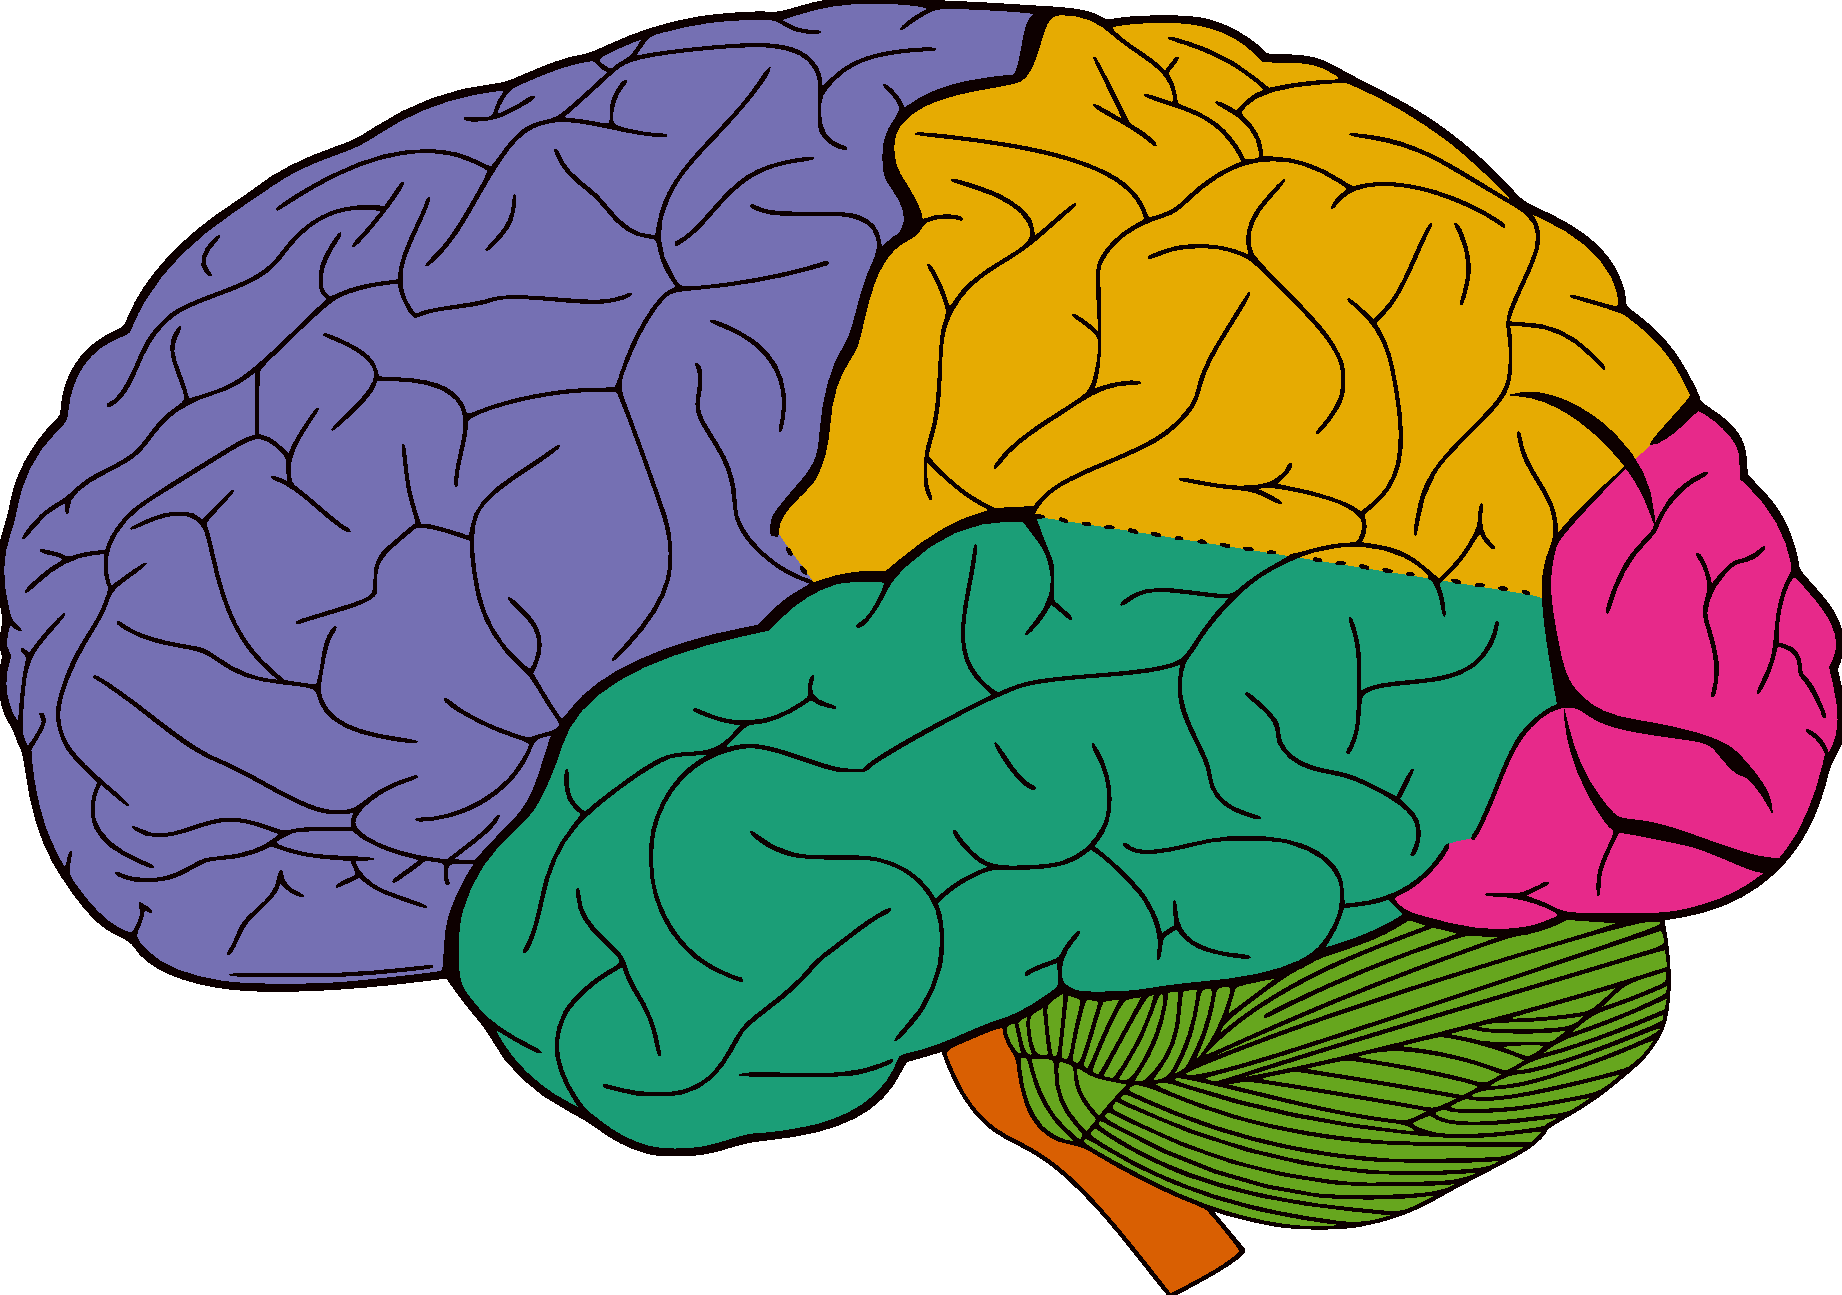
\includegraphics[height=0.3\textwidth]{gfx/neuroanatomy/brain_lobes.pdf}}
\hfill
\tikzset{external/export next=false}
\subcaptionbox{%
        \label{fig:coronalStained}%
        \todo{BB 4201} Coronal section stained for cell bodies. The \ac{GM} is dark while the \ac{WM} is bright. The left and right hemisphere is connected via the corpus calosum.}%
    [0.47\textwidth]{\includegraphics[height=0.3\textwidth]{dev/brain/BB_4201.png}}
    % \begin{tikzpicture}[]
    %     \node[inner sep=0pt, anchor = south west] (fig) at (0,0)
    %     {\includegraphics[height=0.3\textwidth]{dev/brain/BB_4201.png}};
    %     \coordinate (WM1) at ($(fig.north west)!0.6!(fig.north east)$);
    %     \coordinate (WM2) at ($(fig.north east)!0.35!(fig.south east)$);
    %     \draw[RED, ultra thick, <-] (WM1 |- WM2) -- ++ (-42:0.75) node[pos=1, anchor=north] {\textbf{WM}};
    %     \coordinate (GM1) at ($(fig.north west)!0.275!(fig.north east)$);
    %     \coordinate (GM2) at ($(fig.north east)!0.125!(fig.south east)$);
    %     \draw[GREEN, ultra thick, <-] (GM1 |- GM2) -- ++ (-65:0.75) node[pos=1, anchor=north] {\textbf{GM}};
    % \end{tikzpicture}
% }
\caption{Illustration of the human brain and a cell body stained coronal section.}
\label{fig:humanBrain}
\end{figure}
%
The cerebellum and cerebrum contain a \ac{GM} stucture at the brain surface.
This structure is filled with neurons.
These cells have the task of processing the information of all signals coming from inside and outside of the brain.
These cells are arranged in cortical layers that have different thicknesses, cell types, and densities specific to a brain area.
These cells have a relatively high density and are not only locally interconnected with each other, but connect also with different brain areas.
%  (see \cref{fig:nerveFiber,fig:cortLayers}).
Therefore, the folding of the brain is particularly important to increase the surface and therefore the number of cells.
In the human brain there are several billions of nerve cells.
There are many types of cells, \eg{} granule or pyramidal cells.
The highly interconnected structure and arrangement of the various cells is the source of its high number of different functionalities.
It is imporatant to investiagte the human brain to gain a better understanding of the brain's function and an improved understanding of pathophysiological processes that may lead to improved medical treatment of brain deseases.
%
%
%
\section{Fiber architecture} \label{sec:fiberArchitecture}
%
\begin{figure}[!t]
\centering
% \subcaptionbox{
%     \label{fig:cortLayers}
%     Cortical layers \todo{wichtig?}
%     }[0.225\textwidth]{\includegraphics[height=4.5cm]{dev/wiki/layers.png}}
% \hfill
\tikzset{external/export next=false}
% \subcaptionbox{
%     \label{fig:nerveCell}
%     Nerve cell structure.
% }[0.75\textwidth]{
\begin{tikzpicture}[every node/.style={font=\small,},]
    \node[inner sep=0pt, anchor = south west] (fig) at (0,0) {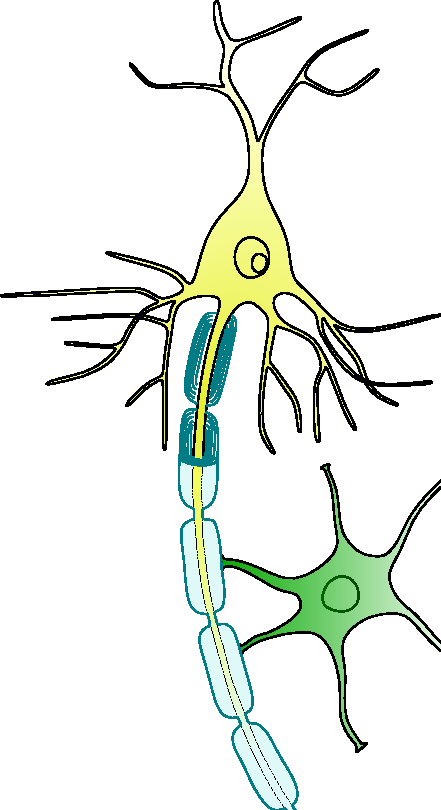
\includegraphics[ angle=90,width=0.75\textwidth]{gfx/neuroanatomy/neuron-axon.pdf}}; %height=4.2cm
    \begin{scope}[overlay]
        % \foreach \p in {0,0.1,0.2,0.3,0.4}{
        %     \draw[blue] (rel cs:name=fig,x=\p,y=\p) rectangle (rel cs:name=fig,x=1-\p,y=1-\p);
        % }
        % 
        \node[anchor=south] at (rel cs:name=fig,x=0.72,y=1.025) {Oligodendrocyte};
        \node[anchor=north] at (rel cs:name=fig,x=0.235,y=0.22) {Cell Body};
        \node[anchor=west] at (rel cs:name=fig,x=1,y=0.675) {Axon};
        \node[anchor=north] at (rel cs:name=fig,x=0.7,y=0.4) {Myelin};
        \draw[<-] (rel cs:name=fig,x=0.9,y=0.5) -- ++(-69:0.5) node[pos=1,anchor=north] {Node of Ranvier};
        \draw[<-] (rel cs:name=fig,x=0.295,y=0.53) -- ++(-140:0.75) node[pos=1,anchor=north] {Nucleus};
        \node[anchor=south] at (rel cs:name=fig,x=0.24,y=0.8) (D) {Dendrites};
        \draw[->] (rel cs:name={D},x=0.3,y=0) -- ++(-155:0.6){};
        \draw[->] (rel cs:name={D},x=0.7,y=0) -- ++(-25:0.6){};
    \end{scope}
    \path[] ($(fig.south west)-(0,0)$) rectangle ($(fig.north east)+(1,0.75)$);
\end{tikzpicture}
% }
\caption{Illustration of a neuron with axon and oligodendrocytes. The olegodendrocyte build up a layered lipid structure up, surrounding the axon. The myelin layers are separated along the axon by nodes of Ranvier.}
\label{fig:CortexAndNerveCell}
\end{figure}
%
Nerve cells are connected by nerve fibers.
A typical nerve cell (see \cref{fig:nerveCell}) comprises a cell body, called a soma, that processes incoming information.
The information arrives via dendrites, which are star-shaped branches.
The axon is the cell's only information output.
It travels through the brain often associated with nerve fiber bundles to its destination, where it connects with the axon terminal to other neurons.
\par
%
The axon is surrounded by a myelin sheath, a lipid layered structure deriving from nearby olegodendrides (see \cref{fig:human-brain}).
The myeling electrically insulates the axon and improves the speed of propagation of the electrical action potential along the axon and also its signal strength.
The diamater of the myelin ranges from about $\SI{0.5}{\micro\meter}$ to several $\si{\micro\meter}$ (see \cref{tag:axonDiameter}).
There are many different types of axons.
Some contain a very thick myelin layer, while others have none.
The high density of axons and myelin makes the brainappear white and is therefore called \ac{WM}, whereas the outer cell bodys appear darker and ist called \ac{GM}.
This color difference is clearly visible in a Nissle stained histological sections (see \cref{fig:coronalStained}).
\par
%
To enhance the contrast of the nerve fibers to the background, staining like Nissle is used to darken the myelin (see \cref{fig:brainMyelinStain}).
This allows to follow small nerve fibers down to individual nerves depending on their myelination degree.
Larger nerve fiber bundles are such dark, that mostly no orientation can be exracted.
\par
% 
\Cref{fig:brainMyelinStain} shows a nissle stained brain section.
% Both single nerve fibers and nerve fiber bundles are visible.
Between neurons, individual nerve fibers form complex reticular structures.
Several nerve fiber bundles trace their paths through the thalamus and are visible as dark structures.
% 
A closer look with an electron microscope into a nerve fiber bundle of the corpus callosum of a rodent is shown in \cref{fig:elecMic}.
The nerve fibers of the $\SI{100}{\nano\meter}$ thin section are densely packed together.
Axon diameter and myelin thickness vary from nerve fiber to nerve fiber.
% 
\begin{figure}[!t]
	\centering
    \tikzset{external/export=false}
    \subcaptionbox{%
        \label{fig:brainMyelinStain}
        Myelin staining of the human thalamus, sagital section. \textcolor{Orange}{Nerve fiber bundle} structures are visiable as as cut structures visible as elliptical dark shape. In between \textcolor{ProcessBlue}{net-like structures} are fromed from individual nerve fibers. \url{http://brainmaps.org/HBP3/h.sapiens/sag/h5thal-myelin/17a}}
    [.49\textwidth]{
        \begin{tikzpicture}[]  
            \node[inner sep=0pt, anchor = south west] (fig) at (0,0)
            {\includegraphics[width=0.49\textwidth, trim=281 152 0 0, clip]{gfx/neuroanatomy/NeuralNet-BrainAtlasDotOrg.png}};
            %  
            \draw[Orange, ultra thick] (rel cs:name=fig,x=0.42,y=0.49) ellipse (0.75 and 0.375);
            \draw[ProcessBlue, ultra thick] (rel cs:name=fig,x=0.7,y=0.3) ellipse (1.1 and 0.7);
            % 
            \draw[white, ultra thick] let
                \p1=(rel cs:name=fig,x=0,y=0), 
                \p2=(rel cs:name=fig,x=0.1041,y=0), 
                \n1={veclen(\x1-\x2,\y1-\y2)}
            in
                ($(fig.south east)+(-0.2,0.2)$) -- ++ (180:\n1) node[above, midway, anchor=south]{$\SI{50}{\micro\meter}$};
        \end{tikzpicture}        
    }
    \hfill
    \subcaptionbox{%
        \label{fig:elecMic} Electron microscope image of a $\SI{100}{\nano\meter}$ thin section of rodent corpus callosum \cite{WALHOVD20142}. The myelin is visible as dark soroundings around the inner axon.}
    [.49\textwidth]{
        \begin{tikzpicture}[]  
            \node[inner sep=0pt, anchor = south west] (fig) at (0,0)
            {\includegraphics[width=0.49\textwidth]{dev/brain/elec_micrograph_rodent_cc.jpg}};
            \draw[white, ultra thick] let
                \p1=(rel cs:name=fig,x=0,y=0), 
                \p2=(rel cs:name=fig,x=0.1347,y=0), 
                \n1={veclen(\x1-\x2,\y1-\y2)}
            in
                ($(fig.south east)+(-0.2,0.2)$) -- ++ (180:\n1) node[above, midway, anchor=south]{$\SI{1}{\micro\meter}$};
        \end{tikzpicture}
    }
\end{figure}
% 
%
%
\section{Axon Literature}
\label{sec:axonMicroscopy}
%
\Cref{tab:axonDiameter} lists the results of the nerve fiber diameter.
The diameter and their standard deviation are region-specific.
The $g_{\mathit{ratio}}$ describes the fraction of the axon to the entire nerve fiber diameter.
From studies with \ac{dMRI} and electron microscopy
\cite{Stikov2015,Dean2016,Mohammadi2015,Cercignani2017,Berman2018,Jung2018} the $g_{\mathit{ratio}}$ is in the range of $\SI{0.6}{}$ to $\SI{0.9}{}$, depending on the region (see \cref{tab:gratio}).
%
\begin{table}[!b]
\centering
\pgfplotstabletypeset[
    thesisTableStyle,
    font=\footnotesize,
    % col sep=comma,
    columns/area/.style={string type},
    columns/mean/.style={string type},
    columns/std/.style={string type},
]{
    area mean std
    {sup. longitudinal fascide} $\SI{0.8}{\micro\meter}$ $\SI{0.2}{\micro\meter}$
    {Unicate/inferior occipital fasc.} $\SI{0.51}{\micro\meter}$ $\SI{0.05}{\micro\meter}$
    {corpus calosum} $\SI{0.69}{\micro\meter}$ $\SI{0.04}{\micro\meter}$
}
\caption{Nerve fiber diameter distribution of the human brain. Mean values over three human brains \cite{Liewald2014}.}
\label{tab:axonDiameter}
\end{table}
%
\begin{table}[!b]
\centering
\pgfplotstabletypeset[
thesisTableStyle,
font=\footnotesize,
col sep=semicolon,
columns={article,cite,gratio},
columns/article/.style={string type, column name=study, column type = {l}},
columns/cite/.style={string type, column name=cite, column type = {l}},
columns/gratio/.style={string type, column name=$g_{\mathit{ratio}}$},
]{data/gratio.csv}
\caption{human $g_{\mathit{ratio}}$ from invivo mri studies.}
\label{tab:gratio}
\end{table}
% 
\cleardoublepage
\setcounter{chapter}{2}
\chapter{Theory}
\label{sec:theory}
% 
\cleanchapterquote{The first principle is that you must not fool yourself and you are the easiest person to fool.}{Richard P. Feynman}{}%\newline
%
\section{Introduction}
The following section lists the physical theories needed to describe the mathematics behind \ac{3D-PLI}. This includes the basic properties of light with the description of their polarization state, the optical models of the tissue, i.e. the nerve fibers and the mathematical description of the experimental setup of \ac{3D-PLI} and the analysis of its signal. The first part of this chapter was written with the help of \cite{demtroeder2, Fliebach2012}.
% 
% 
% 
\section{Electromagnetic Wave}
% 
Light is an electromagnetic wave. Electromagnetism is first fully described by James Clerk Maxwell. He formulated the Maxwell-Equations \cref{eq::maxwell_general}, generalized from the previous work of Johann Carl Friedrich Gau{\ss}, Michael Faraday and Andr\'{e}-Marie Amp\`{e}re and others:
% 
% \begin{align} 
% \begin{split} \label{eq::maxwell_macro}
%     \nabla \cdot \vec{D} &= 4\pi\rho_\text{f}\\
%     \nabla \cdot \vec{B} &= 0\\
%     \nabla \times \vec{E} &= -\frac{1}{c} \frac{\partial \vec{B}} {\partial t}\\
%     \nabla \times \vec{H} &= \frac{1}{c} \left(4\pi\vec{J}_\text{f} + \frac{\partial \vec{D}} {\partial t} \right)
% \end{split}
% \end{align}
% 
\begin{align} 
\begin{split} \label{eq::maxwell_general}
    \nabla \cdot \vec{E} &= \frac {\rho} {\varepsilon_0}\\
    \nabla \cdot \vec{B} &= 0\\
    \nabla \times \vec{E} &= -\frac{\partial \vec{B}} {\partial t}\\
    \nabla \times \vec{B} &= \mu_0\left(\vec{j} + \varepsilon_0 \frac{\partial \vec{E}} {\partial t} \right)
\end{split}
\end{align}
% 
with $\nabla \coloneqq \left({\frac{\partial}{\partial x}}, {\frac{\partial}{\partial y}}, {\frac{\partial}{\partial z}} \right)$ as vector differential operator, $\vec{E}$ as eletric field, $\rho$ as electric charge density, $\varepsilon_0$ as permittivity of free space, $\vec{B}$ as magnetic field, $\mu_0$ as permeability of free space and $\vec{j}$ as electric current density.
% 
The first equation states no electric field can be generated without an electric charge (charge conservation).
The second equation states, magnetic monopoles does not exists. The basic entity of an magnetic field is a dipole.
The third and forth equation show the interconnection of the electric and magnetic fields in space and time.
A change in the electric field yields to a magnetic field and vice versa.
Equation forth additional indicates the creation of a magnetic field from a electric current $\vec{j}$.
The maxwell equation fullfill the continoiut ... $\divergence j + \frac{\partial \rho}{\partial t} = 0$.
This means that neither an electric of magnetc field can be created without either an electric current or a change of electric potential.
%
% \par
% 
\subsection{EM in a vacuum}
% 
In a vacuum this simplifies with $\rho = 0$ and $\vec{j} = \vec{0}$ to:
% 
\begin{align}
\begin{split} \label{eq::maxwell_vacuum}
  \nabla \cdot \vec{E} &= 0 \quad\\
  \nabla \cdot \vec{B} &= 0 \quad\\
  \nabla \times \vec{E} &= -\frac{\partial\vec B}{\partial t}\\
  \nabla \times \vec{B} &= \mu_0\varepsilon_0 \frac{\partial\vec E}{\partial t}
  \end{split}
\end{align}
% 
With 
\begin{align}
\begin{split} 
    \nabla \times \nabla \times \vec{E} = -\nabla \times \frac{\partial \vec{B}} {\partial t} &= -\frac{\partial} {\partial t} \left( \nabla \times  \vec{B} \right)\\
    &= -\varepsilon_0 \cdot \mu_0 \frac{\partial^2 \vec{E}}{\partial t^2} \, ,
\end{split}
\end{align}
% 
the identity $\nabla \times \left( \nabla \times \vec{A} \right) = \nabla(\nabla \cdot \vec{A}) - \nabla^{2}\vec{A}$ and $\mu_0\varepsilon_0 = \frac{1}{c^2}$, with $c$ as the speed of light\footnote{can be derived from Maxwells equation and Lorentz force in a vacuum}, this further simplifies to:
% 
\begin{align}
\begin{split} \label[pluralequation]{eq::maxwell_wave_equations}
  \frac{1}{c^2} \frac{\partial^2 \vec{E}}{\partial t^2} - \nabla^2 \vec{E} &= 0 \\
  \frac{1}{c^2} \frac{\partial^2 \vec{B}}{\partial t^2} - \nabla^2 \vec{B} &= 0
\end{split}
\end{align}
% 
% Another common representation is
% % 
% \begin{align}
% \begin{split} \label{eq::maxwell_wave_equations_box}
%   \Box \ \vec{E} &= 0 \\
%   \Box \ \vec{B} &= 0
% \end{split}
% \end{align}
% 
% with the help of the d'Alembert operator $\Box \coloneqq \partial^a\partial_a = \nabla^2 - \frac{1}{c^2} \frac{\partial^2}{\partial t^2}$.
% 
This also shows that $c^2  \frac{\partial B} {\partial z} = \frac{\partial E}{\partial t} \Rightarrow \vec{E} \cdot \vec{B} = 0$ and therefore the electric and magnetic field components are perpendicular to each other.
Additionally it also means, that space and time are interconnected and that light travels in vacuum with the speed of light $c$.
% 
\subsection{Solving MW Equ in vacuum}
% 
\Cref{eq::maxwell_wave_equations} have the shape of a wave equation and can therefore as known be solved by
% 
% Using the Maxwell equation in vacuum \ref{eq::maxwell_vacuum}, one can find the most simple solution to the differential equation is a wave:
% 
\begin{align}
\begin{split} \label{eq::dgl_solution}
  \vec{E}( \vec{r}, t ) &= g(\phi( \vec{r}, t )) = g( \omega t - \vec{k} \cdot \vec{r} + \varphi)\\
  \vec{B}( \vec{r}, t ) &= g(\phi( \vec{r}, t )) = g( \omega t - \vec{k} \cdot \vec{r} + \varphi )
\end{split}
\end{align}
% 
where $g$ is any well behaved function (continuous and differentiable) and therefore also their superposition.
% 
With the help of
% 
\begin{align}
k = \mathopen| \vec{k} \mathclose| = \frac{\omega}{c} =  \frac{2 \pi}{\lambda}
\end{align}
% 
a planar wave can be descriped by
% 
\begin{align}
\begin{split} \label{eq::plane_wave}
\vec{E}(\vec{r}) &= \vec{E}_0 \cdot e^{ -i \, \vec{k} \cdot \vec{r} }\\
 \vec{B}(\vec{r}) &= \vec{B}_0 \cdot e^{ -i \, \vec{k} \cdot \vec{r} }
\end{split}
\end{align}
% 
with $\vec{k}$ as Wave vector pointing into the travel direction of the light wave.
% 
% 
\subsection{Polarization}
% 
\begin{figure}[!t]
\centering
\setlength{\tikzwidth}{\textwidth}
\inputtikz{gfx/pli/polarization_state}
\label{fig:polarization_state}
\caption{Illustration of light polarization state. Unpolarized light goes throug a linear polarizer which polarizes the light in one direction (w.l.o.g. $E_x$ and $E_y$ in phase). Afterwords it travels though a quarter wave retarder, which turn linear polarized light (of a specific wave length) into circular polarized light, where w.l.o.g. $E_x$ and $E_y$ are $\pi/2$ phase}
\end{figure}
% 
Since the light wave travels into one direction, and the electric field and magnetic field are perpendicular to $\vec{k}$ as well to each other, there orientation is a fundamental property of light called polarization.
Without any additional info, the polarization orientation is conventional in the direction of the electric field component.
% 
A superposition of x and y wave with z equal to direction of propagation yield w.l.o.g. to the general form
\begin{align}
\vec{E}(z,t) &= \begin{pmatrix} E_{0x} \cdot e^{ -i \phi_x } \\ E_{0y} \cdot e^{ -i \phi_y } \\ 0 \end{pmatrix}
e^{ -i (kz - \omega t)}
\end{align}
%
\begin{figure}[!t]
\centering
\tikzset{external/export=false}
%
% \captionsetup[sub]{textfont=normalsize}
% \captionsetup[sub]{position=top, skip=-14pt}
\tikzset{cross/.pic={
\draw[arrows={-Latex[scale=1]}] (-{sqrt(2)},0) -- ({sqrt(2)},0) node[anchor=north]{\small $E_x$};
\draw[arrows={-Latex[scale=1]}] (0,-{sqrt(2)}) -- (0,{sqrt(2)}) node[anchor=east]{\small $E_y$};
}}
%
% \subcaptionbox{}[.3\textwidth]{
\begin{tikzpicture}
\begin{scope}[shift={(0,0)}, local bounding box=A]
\pic at (0,0) {cross};
% \draw[] (0, 2) node[font=\small] () {linear, horizontal};
\draw[very thick, arrows={Latex[scale=1]-Latex[scale=1]}] (-1, 0) -- (1, 0);
\draw[] (0, -2) node () {$\begin{pmatrix} 1&0 \end{pmatrix}$};
\draw[] (0, -2.75) node () {$\begin{pmatrix} 1&1&0&0 \end{pmatrix}$};
\end{scope}
\node[anchor=south west, xshift=-1em] at (A.north west) {\small \textcolor{magenta}{\textbf{(a)}} linear, horizontal};
% }\hfill
% \subcaptionbox{}[.3\textwidth]{
\begin{scope}[shift={(4,0)}, local bounding box=B]
\pic at (0,0) {cross};
% \draw[] (0, 2) node[font=\small] () {linear, vertical};
\draw[very thick, arrows={Latex[scale=1]-Latex[scale=1]}] (0, -1) -- (0, 1);
\draw[] (0, -2) node () {$\begin{pmatrix} 0&1 \end{pmatrix}$};
\draw[] (0, -2.75) node () {$\begin{pmatrix} 1&-1&0&0 \end{pmatrix}$};
\end{scope}
\node[anchor=south west, xshift=-1em] at (B.north west) {\small \textcolor{magenta}{\textbf{(b)}} linear, vertical};
% }\hfill
% \subcaptionbox{}[.3\textwidth]{
\begin{scope}[shift={(8,0)}, local bounding box=C]
\pic at (0,0) {cross};
% \draw[] (0, 2) node[font=\small] () {linear, $\pi/4$};
\draw[very thick, arrows={Latex[scale=1]-Latex[scale=1]}] (-1, -1) -- (1, 1);
\draw[] (0, -2) node () {$\begin{pmatrix} 1&1 \end{pmatrix}$};
\draw[] (0, -2.75) node () {$\begin{pmatrix} 1&0&1&0 \end{pmatrix}$};
\begin{scope}[overlay]
\draw[] (2, -2) node () {Jones};
\draw[] (2, -2.75) node () {Stokes};
\end{scope}
\end{scope}
\node[anchor=south west, xshift=-1em] at (C.north west) {\small \textcolor{magenta}{\textbf{(c)}} linear, $\pi/4$};
% }
% \\[2em]
% \subcaptionbox{}[.32\textwidth]{
\begin{scope}[shift={(0,-5.75)}, local bounding box=D]
\pic at (0,0) {cross};
% \draw[] (0, 2) node[font=\small] () {left circular};
\draw[very thick] plot[domain=0:360,samples=90,smooth] ({cos(\x)},{sin(\x)});
\draw[very thick, arrows={-Latex[scale=1]}] plot[domain=44:45,samples=1] ({cos(\x)},{sin(\x)});
\draw[very thick, arrows={-Latex[scale=1]}] plot[domain=224:225,samples=1] ({cos(\x)},{sin(\x)});
\draw[] (0, -2) node () {$\begin{pmatrix} 1&i \end{pmatrix}$};
\draw[] (0, -2.75) node () {$\begin{pmatrix} 1&0&0&-1 \end{pmatrix}$};
\end{scope}
\node[anchor=south west, xshift=-1em] at (D.north west) {\small \textcolor{magenta}{\textbf{(d)}} left circular};
% }\hfill
% \subcaptionbox{}[.32\textwidth]{
\begin{scope}[shift={(4,-5.75)}, local bounding box=E]
\pic at (0,0) {cross};
% \draw[] (0, 2) node[font=\small] () {right circular};
\draw[very thick] plot[domain=0:360,samples=90,smooth] ({cos(\x)},{sin(\x)});
\draw[very thick, arrows={-Latex[scale=1]}] plot[domain=46:45,samples=1] ({cos(\x)},{sin(\x)});
\draw[very thick, arrows={-Latex[scale=1]}] plot[domain=226:225,samples=1] ({cos(\x)},{sin(\x)});
\draw[] (0, -2) node () {$\begin{pmatrix} 1&-i \end{pmatrix}$};
\draw[] (0, -2.75) node () {$\begin{pmatrix} 1&0&0&1 \end{pmatrix}$};
\end{scope}
\node[anchor=south west, xshift=-1em] at (E.north west) {\small \textcolor{magenta}{\textbf{(e)}} right circular};
% }\hfill
% \subcaptionbox{}[.32\textwidth]{
\begin{scope}[shift={(8,-5.75)}, local bounding box=F]
\pic at (0,0) {cross};
% \draw[] (0, 2) node[font=\small] () {unpolarized};
\draw[] (0, -2.75) node () {$\begin{pmatrix} 1&0&0&0 \end{pmatrix}$};
\begin{scope}[overlay]
\draw[] (2, -2) node () {Jones};
\draw[] (2, -2.75) node () {Stokes};
\end{scope}
\end{scope}
\node[anchor=south west, xshift=-1em] at (F.north west) {\small \textcolor{magenta}{\textbf{(f)}} unpolarized};
%
\path[] ($(A.west)!-0.075!(C.east)$) -- ($(A.west)!1.075!(C.east)$);
\end{tikzpicture}
% }
%
\caption{polarization states, check vector length,\itodo{test speed}} 
\label{fig:polarization_state_vectors}
\end{figure}
%
\Cref{fig:polarization_state_vectors} shows another representation of the polarization sate of a light wave.
It show the component perpendicular to the travelling direction.
Therefore the time variation can be shown on the xy-plane.
Additionally the states can be describe by the Jones or Stokes calculus, later described in \cref{sec:jones,sec:mueller_stokes}.
% 
% 
% 
\subsection{Light in medium}
% 
The Maxwell equations in \dummy{} are described above. They can be solved analog to \dummy{}. This yields to some special behavior, \eg{} the magnetic and electric field component get out of phase.
However here only the two properties of absorption and diffraction are described.
They derivation can be found \eg{} \cite{demtroeder2, Fliebach2012}.
% 
\subsection{Absorption}
% 
\begin{align}
    I = I_0 \exp(-\mu x)
\end{align}
\todo{herleiten}
% 
Beersche law of absorption with $\mu = \frac{4\pi \kappa}{\lambda_0}$ where $\kappa$ is the imaginary part of the complex refractive index.
% 
\subsection{Refraction}
% 
\begin{figure}[!t]
\centering
\setlength{\tikzwidth}{\textwidth}
\inputtikz{gfx/pli/refraction}
\label{fig:optic_refraction}
\caption{Illustration of refraction.}
\end{figure}
% 
Refraction is the property of light to change direction as it passes from one medium to another. This can be shown by using the full Maxwell equations  for non-conductive material, \ie{} $\vec{j} = 0, \rho = 0$, that the differential equating consist out of a primary wave with from atomic medium induced secondary waves, which leads to a reduction of the velocity of the resulting wave. Mathematically this can be described by a complex number $n = c' / c$.
Using this relationship at a boundary surface between two media, one can show that the incident light beam splits into a reflecting and transmitting light wave. The reflecting light wave has the same angle as the incident light beam relative the the surface normal. The transmitting light beam however due to the reduction of the velocity, changes its direction described by the Snellius law
\begin{align}
    n_0 \sin \alpha = n_1 \sin \beta
\end{align}

% 
\begin{align}
\underline{n} = n + i\kappa
\end{align}
% 
\begin{align}
\begin{split}
\vec{E}(z, t) &= \operatorname{Re}\! \left[\vec{E}_0 \cdot e^{i\, (kz - \omega t)}\right] \\
&= \operatorname{Re}\! \left[\vec{E}_0 \cdot e^{i\, (2\pi(n + i\kappa)z/\lambda_0 - \omega t)}\right] \\
&= e^{-2\pi \kappa z/\lambda_0} \operatorname{Re}\! \left[\vec{E}_0 \cdot e^{i\, (kz - \omega t)}\right]
\end{split}
\end{align}\todo{?}
% 
% 
% 
\subsection{Birefingence}
%
\begin{figure}[!t]
\centering
\setlength{\tikzwidth}{\textwidth}
\inputtikz{gfx/pli/retardation}
\caption{Illustration of retardation.}
\label{fig:optic_retardation}
\end{figure}
% 
\begin{figure}[!t]
\centering
\subcaptionbox{}[.49\textwidth]{
\setlength{\tikzwidth}{0.49\textwidth}
\inputtikz{gfx/pli/ellipsoid_a}}
\subcaptionbox{}[.49\textwidth]{
\setlength{\tikzwidth}{0.49\textwidth}
\inputtikz{gfx/pli/ellipsoid_b}}
\caption{birefringence elipsoid}
\label{fig:index_elipsoid}
\end{figure}
% 
Material can have a different refractive index depending on the relative orientation and polarization of the light beam.
This property is known as birefringence.
The refractive index can be described as the refractive index $n_o$ and extraordinary  $n_e$.
Since these two are perpendicular to each other, one can split the light beam into the same perpendicular parts and describe each by its own.
These two light beams, except for the trivial case of a light beam is perpendicular to the surfave, have a different direction.
However for small relative length (hängt von n ab, bzw der phasenänderung) the two light beams leave the material at the same point and recombined at the end.
The change of phase is called birefringence and is described by the difference between the .. and ...
% 
\begin{align}
    \Delta n = n_e - n_o \> .
\end{align}
% 
This .. can be visualized by the index ellipsoid \cref{fig:index_elipsoid}.
The change of the amplitude and phase can be described by the following two vector matrices descriptions.
% 
% 
% 
\subsection{Jones calculus}
\label{sec:jones}
% 
The Jones calculus, introduced by Robert Clark Jones in 1941, describes the polarization state of a light beam by a complex vector $J$:
% 
\begin{align}
    \vec{J} = \begin{pmatrix} E_x \exp(i \phi_x) \\ E_y \exp(i \phi_y) \end{pmatrix}
\end{align}
% 
The amplitude of the perpendicular components are $E_x$ and $E_y$ with their phase $\phi_x$ and $\phi_y$.
Optical elements, which changes the polarization state, such as a polarization filter and retarder, can be desribed by a matrix:
% 
\begin{align}
\begin{split}
\mat{P}_x = 
\begin{pmatrix}
1 & 0 \\ 0 & 0
\end{pmatrix}
, \,
\mat{P}_y = 
\begin{pmatrix}
0 & 0 \\ 0 & 1
\end{pmatrix}
, \,
\mat{M} =
\begin{pmatrix}
e^{i \varphi_x} & 0 \\ 0 & e^{i \varphi_y}
\end{pmatrix}
, \,
\Lambda_{1/4}=
e^{\frac{i \pi}{4}}
\begin{pmatrix}
1 & 0 \\ 0 & -i
\end{pmatrix}
\end{split}
\end{align}
% 
A rotation of an optical element can be achieved by a 2d rotation matrix $\mat{R}$:
% 
\begin{align}
\begin{split}
\mat{M}(\theta )=\mat{R}(\theta )\cdot\mat{M}\cdot\mat{R}(-\theta )
, \>
\mat{R}(\theta ) = 
\begin{pmatrix}
\cos \theta & -\sin \theta \\
\sin \theta & \cos \theta
\end{pmatrix}
\end{split}
\end{align}
% 
% 
% 
\subsection{M\"uller-Stokes}\label{sec:Mueller-Stokes}
\label{sec:mueller_stokes}
% 
Analog to \cref{sec:jones} the M\"uller-Stokes formalism, described by George Gabriel Stokes in 1852, also describes the polarization state (how good is it \dummy{}) of a light beam.
However it does not use the absolute .. but the relative polarization between both components:
% 
\paragraph{Stokes vector}
\begin{align}
\begin{split}
S_0 &= I \\
S_1 &= I p \cos 2\psi \cos 2\chi \\
S_2 &= I p \sin 2\psi \cos 2\chi \\
S_3 &= I p \sin 2\chi
\end{split} \hspace{-6em}
\begin{split}
& \equiv \langle E_x^{2} \rangle + \langle E_y^{2} \rangle \\
%  & = \langle E_a^{2} \rangle + \langle E_b^{2} \rangle \\
%  & =  \langle E_l^{2} \rangle + \langle E_r^{2} \rangle \\
& \equiv \langle E_x^{2} \rangle - \langle E_y^{2} \rangle \\
& \equiv \langle E_a^{2} \rangle - \langle E_b^{2} \rangle \\
& \equiv  \langle E_l^{2} \rangle - \langle E_r^{2} \rangle
\end{split}
, \,
\vec{S} =
\begin{pmatrix} S_0 \\ S_1 \\ S_2 \\ S_3\end{pmatrix}
\end{align}
% 
% \begin{align}
% \begin{split}
% S_0 & \equiv \langle E_x^{2} \rangle + \langle E_y^{2} \rangle \\
%  & = \langle E_a^{2} \rangle + \langle E_b^{2} \rangle \\
%  & =  \langle E_l^{2} \rangle + \langle E_r^{2} \rangle \\
% S_1 & \equiv \langle E_x^{2} \rangle - \langle E_y^{2} \rangle \\
% S_2 & \equiv \langle E_a^{2} \rangle - \langle E_b^{2} \rangle \\
% S_3 & \equiv  \langle E_l^{2} \rangle - \langle E_r^{2} \rangle
% \end{split}
% \end{align}
% 
Therefore the phase can not be described anymore.
However the relative phase information is stored and can be used to describe also polarization states of polarization filters, which can not be described by Jones.
Aanlog to Jones one can formulate the matrices for the optical components:
% 
\paragraph{Linear Polarizer}
\begin{align}
\mat{P}_x=\frac{1}{2}
\begin{pmatrix}
    1 & 1 & 0 & 0 \\
    1 & 1 & 0 & 0 \\
    0 & 0 & 0 & 0 \\
    0 & 0 & 0 & 0
  \end{pmatrix}
, \,
\mat{P}_y=\frac{1}{2}
\begin{pmatrix}
     1 & -1 & 0 & 0 \\
    -1 &  1 & 0 & 0 \\
     0 &  0 & 0 & 0 \\
     0 &  0 & 0 & 0
\end{pmatrix}
\end{align}
% 
\paragraph{retarder}
\begin{align}
\mat{M}=\
\begin{pmatrix}
    1 & 0 & 0 &  0 \\
    0 & 1 & 0 &  0 \\
    0 & 0 & \cos \delta & \sin \delta \\
    0 & 0 & -\sin \delta &  \cos \delta
\end{pmatrix}
\end{align}
% 
\paragraph{Quarter-wave plate (fast-axis vertical)}
\begin{align}
\Lambda_{1/4}=\
\begin{pmatrix}
    1 & 0 & 0 &  0 \\
    0 & 1 & 0 &  0 \\
    0 & 0 & 0 & -1 \\
    0 & 0 & 1 &  0
\end{pmatrix}
\end{align}
% 
\paragraph{Rotation Matrix}
\begin{align}
\mat{R}(\theta)=
\begin{split}
\begin{pmatrix}
    1 &                0 &               0 & 0 \\
    0 & \cos{(2\theta)} & -\sin{(2\theta)} & 0 \\
    0 & \sin{(2\theta)} & \cos{(2\theta)} & 0 \\
    0 &                0 &               0 & 1
  \end{pmatrix}
\end{split}
\end{align}
% 
Analog to \dummy{} rotations are applied by
\begin{align}
\mat{M}(\theta )=\mat{R}(\theta )\cdot\mat{M}\cdot\mat{R}(-\theta )
\end{align}
% 
% \section{Tissue Discretization}
% % 
% By deviding the volume into small diskreticed subvolumes, one can multiply the .. all together and ... (analog Riemann sum)
% \begin{align}
%     \int F \, dt \approx \sum_n F \, \Delta t
% \end{align}
% see simulation?
% 
%  see simulation
% \paragraph{Micro vs Macro:}
% % 
% % \begin{align}
% %   \int_{y_\textit{min}}^{y_\textit{max}} \vec{v}(y) \,dy\\
% %   x = const
% %   y = y(\alpha,x) = tan(\alpha) \cdot x\\
% %   \vec{v}_r = \begin{pmatrix} \cos(\alpha)\\ \sin(\alpha)\\0\end{pmatrix}, \, \vec{v}_p = \begin{pmatrix} 0\\ 0\\1\end{pmatrix}\\
% %   \vec{v}_r = \begin{pmatrix} \cos(\arctan(y/x))\\ \sin(\arctan(y/x))\\0\end{pmatrix}\\
% %   \int_{y_\textit{min}}^{y_\textit{max}} \vec{v}_p(y) \,dy = (y_\textit{max} - y_\textit{min}) \cdot e_z\\
% %   \int_{y_\textit{min}}^{y_\textit{max}} \vec{v}_r(y) \,dy = \int_{y_\textit{min}}^{y_\textit{max}} \cos(\arctan(y/x)) dy \cdot e_x \\
% %   = x\left(\sinh^{-1}(y_\textit{max}/x) - \sinh^{-1}(y_\textit{min}/x)\right) \\
% %   = 2x \left(\sinh^{-1}\left(\frac{2\sqrt{R-x^2}}{x}\right)\right)
% % \end{align}
% % 
% % \begin{align}
% %     % \frac{\oint \vec{v}_z \mathrm{d}A}{\oint \vec{v}_x \mathrm{d}A} = 
% %     % \frac{\int_{-1}^{1}\abs{\vec{v}} \mathrm{d}x}{\int_{-\frac{\pi}{2}}^{\frac{\pi}{2}} \abs{\vec{v}} \cos(\varphi) \mathrm{d}\varphi} =
% %     % \frac{2}{1}
% %     \frac{A_{\Box}}{A_{\circ}} = \frac{4}{\pi}
% % \end{align}
% % 
% \todo{why 2*dn?}
% 
\section{Experimental Setup}\label{sec:expSetup}
%
\begin{figure}[!t]
    \captionsetup[sub]{position=top}
    \setlength{\tikzwidth}{\textwidth}
	\centering
% 	\subcaptionbox{\label{setup-lap} \ac{LAP}}[\textwidth]{
% % 		\resizebox{0.95\textwidth}{!}{
% 		\inputtikz{gfx/pli/pli_setup}
% % 	}
% 	}\\
% 	\subcaptionbox{\label{setup-pm} \ac{PM}}[\textwidth]{
% % 		\resizebox{0.95\textwidth}{!}{
		\inputtikz{gfx/pli/pli_setup_pm}
% % 	}
% 	}
	\caption{Illustration of PLI setup.}
	\label{fig:pli_setup}
\end{figure}
%
% \begin{figure}[!t]
%     % \captionsetup[sub]{position=top}
%     \setlength{\tikzwidth}{0.3\textwidth}
% 	\centering
% 	\subcaptionbox{\ac{LAP}}[.45\textwidth]{\hfill
% 			\inputtikz{gfx/pli/pli_detail}\hfill}\hfill
% 	\subcaptionbox{\ac{PM}}[.45\textwidth]{\hfill
% 			\inputtikz{gfx/pli/pli_detail_pm}\hfill}
% 	\caption{Illustration of \acs{3D-PLI} setup.}
% 	\label{fig:pli_detail}
% \end{figure}
%
The \ac{3D-PLI} setup is described in \cite{Axer2011} with the tiltable light beam microscope (LMP) in \cite{Wiese:887678}.
For the routine measurements two (three) microscope systems are currently in use.
The first use of a high throughput microscope is the \ac{LAP} with a pixel size of about \SI{60}{\micro\meter}.\footnote{can be change by the optic also to $\SI{40}{\micro\meter}$ and $\SI{20}{\micro\meter}$, but remains for the routine measurements with $\SI{60}{\micro\meter}$.}
It consist out of a led light source (\SI{525}{\nano\meter}), a rotatable polarization filter, a rotatable quarter wave retarder, the specimen stage, which can be tilted for oblique views, a rotatable polarizer.
Both polarizer and quarter wave retarder are rotated at the same time.
The both polarizers have a phase offset of $\SI{90}{\degree}$, the first polarizer and the quarter wave retarder of $\SI{45}{\degree}$ (see (see \cref{setup-lap}).
The second system \ac{LMP3D} microscope fullfills the same measurments, however the retarder is placed after the tissue specimen and fixed with the polarizer without any rotations (see \cref{setup-pm}).
Mathematically it measures the same signal.
\footnote{The rotatable filters of the \ac{LAP} has the advantage, that noise like dust particles can be easy identified and removed. Since the microscop is in a more confined "box" this is not necesarry.}
A difference is that the optical path is in reverse to the \ac{LAP} system.
Since there is a mirror in the path, the image is flipped again so that the coordinate systems stays the same (see \cref{fig:pli_detail}).
% 
\subsection{Signal}
% 
From the M\"{u}ller Matrices (\cref{sec:Mueller-Stokes}) as shown in \cite{MenzelMaster,MenzelDissertation}, that the intensity signal, measured by the \ac{CCD}-sensor, follows a sinusiodal curve:
% 
% \begin{align}
% I = \underbrace{\frac{I_0}{2}}_{\mathclap{\mathit{transmittance}}}
%     \bigl[ \sin\bigl(2\rho - 2{\underbrace{\vphantom{\frac{I_0}{2}} \varphi}_{\mathclap{\mathit{direction}}}} \bigr)
%     \cdot \sin \bigl( {\underbrace{\vphantom{\frac{I_0}{2}} 2\pi\frac{d \dn}{\lambda} \cos^2\left( \alpha \right)}_{\mathclap{\delta \, \coloneqq \, \mathit{retardation}}}} \bigr) \bigr]
% \end{align}
\begin{align}
\label{eq:pli_signal}
\begin{split}
I(\rho, \varphi, \alpha, d) =\frac{I_0}{2}\bigl[ \sin\bigl(2\rho - 2\varphi \bigr)\cdot \sin \bigl( 2\pi\frac{d \dn}{\lambda} \cos^2\left( \alpha \right) \bigr) \bigr] \\
\text{with} \enspace \delta \coloneqq 2\pi\frac{d \dn}{\lambda} \cos^2\left( \alpha \right) \enspace 
\text{and} \enspace \trel \coloneqq \frac{d \dn}{\lambda}
\end{split}
\end{align}
% 
Since \cref{eq:pli_signal} describes a sinosoidal signal, the fourier analysis is a obvious choise.
For a discrete, aquidistant measurement of the rotation angles $\rho$, one can use the fourier series with the three coefficients to describe the signal:
% 
% \begin{align}
% \begin{split}
% A \sin(\omega t + \alpha) + B \sin(\omega t + \beta) &= \sqrt{C^2 + D^2} \cdot \sin \, \left( \omega t + \tan^{-1} \left( \frac{D}{C} \right) \right)
% \end{split}
% \\
% \begin{split}
% C &= A \cos(\alpha)+ B \cos(\beta)\\
% D &= A \sin(\alpha)+ B \sin(\beta)
% \end{split} \nonumber 
% \end{align}

\begin{align}
\begin{split}
\rho &= [\SI{0}{\degree}, \frac{1\cdot180}{N+1}\si{\degree}, \frac{2\cdot180}{N+1}\si{\degree}, ..., \frac{N\cdot180}{N+1}\si{\degree}]\\
a_0 &= \frac{1}{N} \sum(\mathit{data})\\
a_1 &= \frac{2}{N} \sum(\mathit{data} \cdot \sin(2 \cdot \rho)\\
b_1 &= \frac{2}{N} \sum(\mathit{data} \cdot \cos(2 \cdot \rho)
\end{split}
\end{align}

With these the final \ac{3D-PLI} modalities are calculated:

\begin{align}
\begin{split}
\mathit{transmittance} &= 2 \cdot a_0\\
\mathit{direction} &= 0.5 \cdot \atantwo(-b_1 / a_1)\\
\mathit{retardation} &= \frac{\sqrt{a_1^2 + b_1^2}}{a_0}
\end{split}
\end{align}
% 
\itodo{Section Images}
% 
% 
% 
\subsection{Inclination analysis}
% 
To be able to analyse the inclination $\alpha$ one has to distinguish the relative strength of the birefringence from the $\cos^2(\alpha)$.
For this purpose a tiltable specimen was developed, which allows measuring the light signal through the tissue with a different angle of incidence.
This mean, that tissue and therefore the nerve fibers also change their orientation by the tilting angles $\theta, \varphi$.
Additionally the distance the light travels through the tissue, elongates by $1/\cos(\theta)$ \cref{fig:tilted_side_view}.
% 
Depending on the \pixelsize{}, this light travels though the same volume, but with another orientation.
Therefore a measurement of multiple light paths can be ... and the resulting signals can be used to analyse the inclination and relative birefrigente tissue thickness \trel{}.
The angle of incidence on the glass ... and the tissue also changes the angle of the light by Snellius law.
All angles mention here are if not specified always the change of angle of the light inside the tissue (see \cref{fig:tilting_camera_view}). 
This also leads to a perspective shift, which has to be corrected by a registration process.
In this case an affine transformation.
This effect is however neglected in the simulation, since it only adds a parallel offset.
% 
In \cite{Schmitz2018} this analysis published under the name of \ac{ROFL}, which builds up on the work of \cite{Wiese:887678}.
The idea is to fit the measured signals of all light paths simultaniously.
Because the change of signal is proportional to the $\cos(\alpha)$ this however means, that for steep fibers, the changes are not only small, but also the amplitude of the signal is very small.
This leads to the problem of increasing uncertanty with increasing inclination angle.
\\
A further problem is that for a smaller \pixelsize{} the light path cannot be neglected anymore.
For the \ac{LMP3D} system this means, that with a maximal tilting angle of about $\SI{3.9}{\degree}$ and a usually tissue thickness of $\SI{60}{\micro\meter}$ the light path is measured in n \dummy{} pixels away from the non tilting case, if the rotation point is in the center of the tissue.
\\
For homogeneous tissue regions like parts in the dense \ac{WM}, this can be ignored.
For single fiber paths in the \ac{GM} however this is currently an unsolved problem.
% 
% 
% 
\section{Orientation visualization}
% 
\begin{figure}[!t]
\centering
\setlength{\tikzwidth}{0.4\textwidth}
\begin{center}
\begin{tabular}{m{6cm}m{6cm}}
\includegraphics[width=\tikzwidth]{gfx/pli/color_sphere.png}
&
\inputtikz{gfx/pli/hsv_sphere}
\\
\begin{minipage}[t]{0.42\textwidth}
\leavevmode\subcaption{2d hsv sphere}
\end{minipage}
&
\begin{minipage}[t]{0.42\textwidth}
\leavevmode\subcaption{\label{fig:sphere}3d hsv sphere}
\end{minipage}
\end{tabular}
\end{center}
% 
\vspace{-1em} % because of tabular?
\caption{collor spheres}
\label{fig:spheres}
\end{figure}
% 
% 
The orientation of the birefringence axis is descibed by the direction angle $\varphi$ and inclination angle $\alpha$ (see \cref{fig:sphere}).
To be able to show a 3d information, the \textit{hsv-black} is usually shown in \ac{3D-PLI}.
It color code the orientation by:
\begin{align}
\begin{split}
    H &= \varphi/\pi\\
    S &= 1\\
    V &= 1-\alpha / \pi/2
\end{split}
\end{align}
This way the color corresponds to the direction, and the color value to the inclination.
Since the orientation, unlike a vector, covers only a half sphere, the colors are point symmetric.
% 
\itodo{Section Images}
% fig:spheres
% 
% 
\section{optical resolution}
\label{sec:opticalResolution}
% 
The optical resolution of an imaging system describes the minimal size of on object which can still be resolved.
This property is limited by aberration and diffraction which both cause a blurring of the resulting image.
Ernst Abbe described as on of the first that the resulition corrlates with the lightwave $\lambda$: 
\begin{align}
d=\frac{ \lambda}{2 n \sin \theta} = \frac{\lambda}{2\mathrm{NA}} \> .
\end{align}
$d$ is the minimal resolvable distance, $n$ the refractive index, $\theta$ the angle of a spot light, which can be combined to the better known numerical aperture $\mathrm{NA}$.
This results in an absolute threshold for a light microscope above which the resolution can no longer be improved.
For the wavelength used in \ac{3D-PLI} with $\lambda = \SI{525}{\nano\meter}$ and a numerical apperatur of $\mathrm{NA} = \SI{}{}$ this yields to a limit of \dummy{}.
% 
\begin{figure}[!t]
\setlength{\tikzwidth}{0.45\textwidth}
\centering
% \subcaptionbox{}{
\inputtikz{gfx/pli/rayleigh}
\caption[Raylay criterium]{rayleigh criteria. The minima of the one function is in the maxima of the other.}
\label{fig:rayleigh}
\end{figure}
% 
% 
% 
% 
\section{Computational speedup techniques}
% 
Among other already mentioned techniques, \eg{} the use of an octree, two main optimisation techniques are used to speed up the process., be placed before a dash. Whe
% 
\paragraph{Memory alignment}\todo{more general, myby fastpli package}
The \code{std::vector} has the advantage that the data is linear in memory.
Modern \acp{CPU} have a built-in method called \say{ache prefetching}.
Data must be prepared and sent from the \ac{RAM} to the cache of the \acp{CPU}.
This takes time.
The main advantage of the cache is that it is very fast.
However, since it must be very close to the \ac{CPU}, the cache is very fast. (in modern systems the speed is already limited by the speed of light) its size is very limited (usually around $\si{\mega\byte}$).
The prefetcher is an ingenious directive, which not only obtains the item at address $i$ in memory, but also the item next to it ($i+1$ or $i-1$ depending on the algorithm).
Since many algorithms pass through arrays, the next item to be calculated is usually the next (or previous) item.
Therefore the time needed to copy the data into the cache and prepare it is reduced.
It can be shown that for linear operations on the memory the cache prefetcher reduces the time so much that it behaves as if the \ac{CPU} has an infinite cache.
% 
% 
\cleardoublepage
\part{Software}
% \acbarrier
\parttoc
\setcounter{chapter}{4}
\chapter{Modelling}
\label{chap:modelling}
% 
\section{Introduction}
\comment{
\cite{Balls2009}
% 
\begin{itemize}[nosep]
    \item current techniques
    \item their limitations
    \item collisions
    \item link to \cite{matuschke2019}
\end{itemize}}
% 
\vspace{5pt}
\hrule
\vspace{6pt}
% 
\comment{
\begin{itemize}[nosep]
    \item test
\end{itemize}
}
% 
\vspace{5pt}
\hrule
\vspace{6pt}
% 
Nerve fiber modelling is a non trivial task, which is \comment{(mainly?)} used in simulations like \ac{dMRI} simulations \dummy. However most \ac{dMRI} simulation tools use fast simulation techniques as \dummy. This take analytical function describing the fiber paths to be capable of calculation very fast.
% 
In resent time with the improvement of computer power and algorithms, simulators like monte carlo are used \dummy. These simulate the random walk of individual water molecules inside a volume. If the target are \ac{WM} phantoms nerve fibers can be modelled as a meshed tube.
These have the advantage, that any complex configuration can be modelled \eg beeding fibers \dummy.\\
%
However a disadvantage is that for resanable model sizes ( in \ac{dMRI} a voxel is about \SIrange{100}{1000}{\micro\meter} order, size nerve fiber about \SI{1}{\micro\meter}), the number of triangles of the mesh is quite big.
A further ... is to build a geometrical configuration, where no nerve fibers are overlapping each other (\ie  take the same volume in space). \\
% 
Collision detektion takes a major role here.
When other simulations using geometrical models (\eg protein folding \dummy) can use something like electric potentials, where the actuall geometrical boundry is not that important, here it is different.
Collision detection algorithms are manly used for computer \dummy.\\
% 
Inside this chapter the following procedures are described:
\begin{itemize}[nosep]
    \item geometrical representation of nerve fiber (bundles)
    \item user friendly building methods
    \item ensure collisionless models
\end{itemize}

\paragraph{Module}
% 
The python sub package \pymodule{fastpli.model} consist of two modules:
% 
%\vspace{-1ex}
\begin{itemize}[nosep]
    \item \pymodule{sandbox}
    \item \pymodule{solver}
\end{itemize}
% 
The first module \pymodule{sandbox} enherets routines to help the user build simple geometric configurations.
Ths can then be used to build more complex structres of nerve fiber bundles.
The second module \pymodule{solver} contains a \CXX framework wrapped inside a \python class to ensure easier user \ac{API} (see \dummy).

\section{Nerve Fiber representation}
% 
As described in \cref{sec:fiberArchitecture} \ac{WM} consist of densly Axons which are surrounded by Myeling (see \cref{fig:nerveFiber}).
The Myelin itself is split into several parts separated by Nodes of Ranvier, to allow the propagation of an action potential.\\
% 
How to represend such a "tube" is known for a long time. A common representation is a triangulared mesh representation (e.g. mri simulation \dummy). Since the goal of the later use is to acount for collisions between fibers, it is importeant to minimize the number ob "objects" as much as possible. However since a nerve fiber is relativly fexible it is a tradeoff between accurate representation and number of objects (later speed).
% 
For the purpose of collision solvin it was decided, to chunk a single nerve fiber into segments, which are themself conical objects.

This allows a complex trajectory $f(t) \rightarrow \left(\vv{p}=(x,y,z),r\right)$ (depending on the segment length) it is however necessary, to split the cylinder in smaller segments. Since the radii of a nerve fiber is naturally changing along its trajectory, a \ac{CC} shape is best to use ass segment geometry.
Two coordinates $(p_i, p_{i+1})$ and radii $(r_i, r_{i+1})$ are assigned to each segment. Two neighbouring segment share there parameters.
Therefore a list of tuples containing four floating point numbers can be interpret as fiber (\cref{fig:fiberReb}):
\begin{align}
\begin{split}
\mathit{fiber} &= \left\{ \vv{p}_i=(x_i,y_i,z_i), r_i \mid i \in \{0,1,N_{\mathit{points}}-1\}\right\} \\
\mathit{segment}_i &= \left\{ \vv{p}_i, \vv{p}_{i+1}, r_i, r_{i+1} \mid i \in \{0,1,N_{\mathit{seg}}-1\} \right\}
\end{split}
\end{align}
% 
% This representation will also be used for visualization (see \dummy).
% 
\begin{figure}[!t]
    \def\tikzwidth{0.85\textwidth}
    \centering
    \inputtikz{gfx/model/fiber_model}
	\caption[]{representation of nerve fiber from a list of spheres $\left\{ \vv{p}_i=(x_i,y_i,z_i), r_i \mid i \in \{0,1,N_{\mathit{points}}-1\}\right\}$.}
	\label{fig:fiberReb}
\end{figure}
% 
% 
% This allows to represent a nerve fiber by a chain of cylinders:
% \begin{align}
% \mathit{fiber} = \left\{ \mathit{cylinder}(\vv{p_i}, \vv{p_{i+1}}, r) \mid i \in \{0,1,N_{\mathit{seg}-1}\} \right\}
% \end{align}
% % 
% This already allows the change of radii along the fiber trajectory.
% However when the fiber change is orientation along its trajectory, there would be a junction between two cylinders.
% This can be fixed by using capsule (cylinders with spherical endings) instead of cylinders:
% \begin{align}
% \mathit{fiber} = \left\{ \mathit{capsule}(\vv{p_i}, \vv{p_{i+1}}, r) \mid i \in \{0,1,N_{\mathit{seg}-1}\} \right\}
% \end{align}
% % 
% This representation works quite well for non changing fiber radii $r_i$.
% If the radii is changing, the next logical step is to change the geometry from a capsule to a \ac{CC}.
% \begin{align}
% \mathit{fiber} = \left\{ \mathit{cone_{cap}}(\vv{p_i}, \vv{p_{i+1}}, r_i, r_{i+1}) \mid i \in \{0,1,N_{\mathit{seg}-1}\} \right\}
% \end{align}
% % 
% \begin{figure}[!t]
%     \def\tikzwidth{0.85\textwidth}
%     \centering
%     % \subcaptionbox{cylinder}[\textwidth]{
%     % \inputtikz{gfx/model/cylinder}}
%     % \subcaptionbox{capsule}[\textwidth]{
%     % \inputtikz{gfx/model/capsule}}
%     % \subcaptionbox{conical capsule}[\textwidth]{
%     \inputtikz{gfx/model/conical_capsule}
%     % }
% 	\caption[]{crossing bundles. Noch mist}
% % 	\label{fig:}
% \end{figure}
% % 
% This representation allows a smooth change in volume along the trajectory dependend on the number of segments and their individual length.
% 
\section{Sandbox}
% 
Two major processes are typical, when building white matter phantom. First, defining macrostructures like fiber bundles, second, defining fibers inside the fiber bundles.
Defining a fiber bundle can be as easy as defining a fiber, if the shape should by tube like as well.
\\
To populate the fiber bundle, the following technique was developed.
% 
\subsection{seeds}\label{sec:seeds}
% 
Seeds are a list of 3d points related to a coordinate center $(0,0,0)$ (see \cref{fig:triGrid,fig:rndGrid}).
This list can be applied to a a trajectory.
% 
\begin{figure}[!t]
    \def\tikzheight{0.25\textwidth}
    \centering
    \subcaptionbox{\label{fig:triGrid}equilateral triangle grid}[.295\textwidth]{
    \inputtikz{gfx/model/triangular_grid}\hfill}
    \subcaptionbox{\label{fig:rndGrid}random grid}[.295\textwidth]{
    \inputtikz{gfx/model/rnd_circle_points}}\hfill
    \subcaptionbox{\label{fig:crossBundle}populated fiber bundles}[.39\textwidth]{
    \inputtikz{gfx/model/crossing_bundle}\hfill}
	\caption{Populating fiber bundles with seed points.}
% 	\label{fig:}
\end{figure}
% 
\subsection{cube models}
% 
Since \ac{3D-PLI} is a technique, which uses brain sections, and the camera signals result in 2d images, a method was implemented to build fiber bundles inside a 3d cube.
The method works similar to populate a bundle with seeds (see \cref{sec:seeds, sec:fillBundle}).
The population orientation is defined by a orientation vector $\vv{v}$;
% 
\subsection{cylindric models}
% 
building a cylindric model works the same way as cube models.
The cylinder is definde by a vector $\vv{v}$ wich gives the orientation and length of the cylinder.
A inner and outer radii $(r_{\mathit{in}}, r_{\mathit{out}})$ has to be defined as well.
Inside the inner and outer radii the cylinder will be populated $\{f_i \mid r_{min} < |(s_{i,x},s_{i,y})| < r_{max} \}$.
Additionally a beginning end ending angle $(\alpha, \beta)$ can be defined, which let the cylinder only fill from $\alpha$ to $\beta$.
Last the cylinder can be modelled in three ways. a) parallel, b) cylindrical and c) radial to the cylinder orientation (see \dummy).
% 
\subsection{Populate bundles}\label{sec:fillBundle}
% 
\begin{figure}[!t]
    \centering
    \resizebox{0.75\textwidth}{!}{
    \includegraphics{dev/gfx/circle_bundle.png}}
	\caption[]{Bending fiber along trajectory $f(t) = \left( \cos(t), \sin(t), 0 \right)$}
	\label{fig:circleBundle}
\end{figure}
% 
\begin{figure}[!t]
    \def\tikzwidth{0.75\textwidth}
    \centering
    \inputtikz{gfx/model/min_torsion}
	\caption[Minimal torsion trajectory]{Minimal torsion along trajectory. The 
	\textcolor{green!50!black}{binormal}, \textcolor{red}{principal normal} vector and \textcolor{blue}{tangent vector} vector at each step are also the coordinate system for the seed points.}
% 	\label{fig:}
\end{figure}
% 
Populating a \say{bundle} is is done via moving the \say{cloud} of seed points along the trajectory, moving,bending/rotating smooth along its way (like a good rolercoster).
The trajectory of each individual seed point will then be interpret and returned as a individual fiber with a constant single radius, or individual radii (wich can later be changed if necessary).
The distant of the seeds to their coordinate center can be scaled with the bundle \say{radii} or scale factor (set 1 for const). \comment{energy minimum?}:
% 
\begin{align}
\begin{split}
\vv{f}(s) &= (x(s),y(s),z(s)) \\
\vv{t}(s) &= \vv{f}\,'(s) \\
\vv{n}(s) &= \frac{\vv{t}\,'(s)}{|\vv{t}\,'(s)|} = \frac{\vv{r}\,''(s)}{|\vv{r}\,''(s)|} \\
\vv{b}(s) &= \vv{t}(s) \times \vv{n}(s)
\end{split}
\end{align}
% 
However, for a constant fiber trajectory (e.e. $f(s) = (s,0,0,1)$) $\vv{n}$ and $\vv{b}$ are not defined. There are alternatives like a minimal twisting frame. But this would mean, that \eg a fiber bundle would twist along a const path. This could be, but is not likely.
\\
% 
Therefore it was decided to use another teqchnique. Its originates from the idea, that the tangential vector $\vv{t}$ should move by a single rotation matrix as fast as possible from $\vv{t}_i$ to $\vv{t}_{i+1}$. This can be also interpret as that the tangential vector on a sphere takes the geodic line to its next point. The same rotation matrix is then used for the $\vv{n}$ and $\vv{b}$ vector. The initial $\vv{n}$ and $\vv{n}$ correspont to the $\vv{e}_x$ and $\vv{e}_y$ of the seed points coordinate frame.
% 
\section{\VCS}
% 
\begin{figure}[!t]
    \centering
    \def\tikzwidth{0.75\textwidth}
    \inputtikz{gfx/model/conical_capsule_bb}
    \tikzset{external/export=false}
	\caption[cc and co]{\Acf{CC}: \raisebox{.25em}{\tikz \draw[black](0,0)--(0.275,0);} \ac{CC}, \raisebox{.25em}{\tikz \draw[blue, dash pattern=on 2.5pt off 2.5pt](0,0)--(0.275,0);} capsule, \raisebox{.25em}{\tikz \draw[red, dash pattern={on 2.5pt off 0.9pt on 0.42pt off 0.9pt}](0,0)--(0.275,0);} bounding box}
	\label{fig:conical_capsule}
\end{figure}
% 
This Method aims to model densly \ac{WM}.
The main component inside \ac{WM} consist of an Axon and its surrounding Myeling [see \dummy].
The Myelin itself is split into several parts to allow the propagation of the action potential at the Nodes of Ranvier. \\
% 
This structure is modelled as a chain of capsules, a cylinder with hemispherical ends \cref{fig:conical_capsule}.
To allow a change of cross section or radii, the capsule ending are allowed to consist of individual radii.
The resulting shape will be referred to as a \ac{CC}.
The chain of \ac{CC} consist therefore of a list of 3d points with individual radius. \\
% 
To model flexible and curved densly packed nerve fibers, a collision free result needs to be obtained.
The representaion of nerve fibers by \ac{CC} allows a fast calculation if two \ac{CC} are colliding each other. \\
% 
However instead of building a collision free model, which is quite impossible for a \dummy structure, the strategy is to initialize a model, checking for collisions and then solving these collisions by pushing the fiber or \ac{CC} slightly apart. \\
% 
This allows a user to specify any initial configuration and reaching a collision free model, which, depending on the initial overlap, follows the initial geometry.
The disadvantage obvious is that the configuration has to change.
However since biological tissue is deformable and not "caotic" itself, it follows its natrual behavier.
%
% 
% 
\section{Collision Detection}
% 
Collision detection for a large number of objects is a very computational intense algorithm.
To reduce the computational afford, the \ac{CC} will be interpreted as a capsule object, since this alows a much simpler calculation.
The capsule has the radius $r_{\text{capsule}} = \max(r_0, r_1)$ to soroun the hole \ac{CC}.
To check if two capsules collide with each other the distance between the line segments, defined by the capsule begin and end points $p_0, p_1$, is calculated.if the distance $d$ is $d < (r_0 + r_1)$ then the two capsule objects are colliding each other. \\
% 
To calculate the smallest distance between two line segemnts, sevverel algorith,s already exists.
A fast approach was chosen\footnote{\href{https://www.john.geek.nz/2009/03/code-shortest-distance-between-any-two-line-segments/}{https://www.john.geek.nz/2009/03/code-shortest-distance-between-any-two-line-segments/}}.
%
\section{World}
For a given cuboid volume the computing grows $\mathcal{O}(V^3)$.
Furthermore each object has to be checked to each other, therefore the number of objects to be checked for a collision grows by $\mathcal{O}(n^2)$.
This explodes rather quick.
In the literature are several approuches (e.g. computer games industry).
However since the number of objects will be $\approx \num{e9}$ \dummy cant be used. \\
% 
A "tree" is a data structure consist of a collection of "nodes", which are connected to each other.
One node is conected toword the "root" with a single parent node and towords the "branches" with several "children" or "branches".
The nodes at the end of a branch are refered to as "leafs" wich contain the data.
Traversing a  evenly distributed tree is of $\mathcal{O}(\log(n))$.\\
% 
\begin{figure}[!t]
    \centering
    \subcaptionbox{oct tree}[.3\textwidth]{
    \def\tikzheight{0.6\textwidth}
    \inputtikz{gfx/model/oct_tree}}
    \subcaptionbox{collision 2d}[.65\textwidth]{
    \def\tikzheight{0.6\textwidth}
    \inputtikzext{gfx/model/collision_tree}}
	\caption{}
	\label{fig:oct_tree}
\end{figure}
% 
An octtree is a special kind of tree where each node contain 8 children.
This allows to divide a cubic volume into 8 equal cutted subcubes.
Therefore this data structure was chosen to reorder the fiber segents.
To order them, a recursive function is used.
It checks, if the number of objects is below a threshold $n < t_n$, or the subvolume cube length is below a threshold $dim < t_{dim}$.
If so, the leaf is reached and all objects are check for collision with each other.
Otherwise a 8 new subvolumes will be created and each object will be check, if it is inside upto 8 of the new created volumes.
The next branch will check only with the new includes objects. \\
% 
This allows a rather quick reduction of number of objects to be checked.
Therefore the last step with an $\mathcal{O}(n^2)$ is not that painful anymore.
To speed up the calculation, The objects itself wont be duplicated.
All objects are contained in a \textit{std::vector} of cones.
Only the indices will be transfered to the next recursive function call.
Also the objects are traversed in order, so that the maximum speed from the cpu cache can be exploited. \\
% 
The minimal subvolume size is choses to $\sqrt{3} \times \max(\mathit{object\_size})$.
Smaller then this would only replicated subvolumes with identical contained objects.
The maximum number of objects is set to \num{25} objects \footnote{found suitable by testing.}. \\
% 
The building of the tree is don in parallel.
Up to 8 threads are spawned to check for the first 8 subvolumes, which objects are contained.
The next level can again spawn upto 8 new threads (64 in total).
This compensates if a the objects are not uniformly distributed.
After the first level, each cpu thread traverses it branch.
At each leaf a list ob object is returned containing the object of the leaf.
All list are collected for the collision checking test.
This collected list is in the next step fully parallel traversed to check for collisions.
% 
\subsection{Solving a collision}
To solve a collision between two \ac{CC} objects the two points of each object will be moved.
The movement will be parallel to the smallest distance line between both objects.
To take the 3d placement into consideration, the movement is weighted with the distance of the the individual points to the intersection point with the smallest distance line (see fig \dummy).
This will result in a more controlled movement if \eg only the two endings of the fiber objects collide each other. \\
% 
The movement is saved for each object in a velocity \textit{std::vector}.
Therefore the sum of all velocities is taken into account.
The maximum speed is however limited to a value of $v_{\max} = 0.1 \times \min(\mathit{object radius})$.
This prevents movement through another object.
% 
\subsection{Shape Control}\label{chap5:ShapeControl}
The movement of individual points can results in a "distorted" fiber model, \eg two points move very far apart from each other.
Therefore boundry conditions have to be specified.
It was decided to use the following two conditions:
% 
\subsubsection{Mean segment length}
% 
\begin{figure}[!t]
    \centering
    \def\tikzwidth{.42\textwidth}
    \subcaptionbox{merge}[.49\textwidth]{
    \inputtikz{gfx/model/model_merge}}
    \subcaptionbox{split}[.49\textwidth]{
    \inputtikz{gfx/model/model_split}}
	\caption{Length control for fibers $f$ and $f'$}
	\label{fig:merge_split}
\end{figure}
% 
% 
\begin{figure}[!t]
    \centering
    \def\tikzwidth{\textwidth}
    \tikzset{external/export next=false}
    \inputtikz{gfx/model/model_length}
	\caption{different fiber segment length.}
	\label{fig:model_length}
\end{figure}
% 
The Mean segment length coresponts to the distance between the two points of an object.
If the lenght of the object becomes to small/big, the points inside a fiber coresponding to the object are merged/splitted resulting in one point less / adding a new point.
The minimum/maximum distance of the object is set to $d_{\min} = \frac{2}{3} \overline{d}, d_{\max} = \frac{4}{3}\overline{d}$.
Therefore the mean allowed value of the object is $\frac{d_{\min} + d_{\max}}{2} = \overline{d}$. \\
% 
If a new point is created due to exceeding the maximum limitation, the new points position $\vv{p}_{new}$ is 
\begin{align}
\begin{split}
\vv{p}_{new} &= \frac{\vv{p}_{i} + \vv{p}_{i+1}}{2}\\
r_{new} &= \frac{r_{i} + r_{i+1}}{2}\\
\vv{v}_{new} &= \frac{\vv{v}_{i} + \vv{v}_{i+1}}{2}
\end{split}
\end{align}
with a radius of $r_{new}$ and a velocity $\vv{v}_{new}$.
% 
\subsubsection{Bending radius}
% 
The bending radius is defined as the circular radius corresponding to the circle defined by three neighbouring points $p_{i-1}, p_{i}, p_{i+1}$. 
The limit is set as a minimal radius of $r_{\min}$.
If a point $p_{i}$ in a fiber fall below this value, the three points will be moved.
$p_{i-1},p_{i+1}$ will be moved \dummy and $p_{i}$ oposit.
Therefore the curvature will be reduced.
% 
\begin{figure}[!t]
    \centering
    \def\tikzheight{.40\textwidth}
    \subcaptionbox{Boundry segment length: lower bound $phi=\SI{60}{\degree} \xrightarrow{} r_{min} \geq \SI{0.5773}{} \cdot l_{mean}$}[.475\textwidth]{
    \inputtikz{gfx/model/model_circle}}\hfill
    \subcaptionbox{Boundry segment radii: lower bound $r_{min} \geq \fiberRadiusMean $}[.45\textwidth]{
    \inputtikz{gfx/model/model_circular}}
	\caption{Geometrical boundry condition for fiber segment length \segLength and fiber bending radius \segRadius.}
	\label{fig:model_circle}
\end{figure}
% 
\newline
Both movements are added to the velocity vector before performing the overall movement.
The algorithm performs each step sequentially (see \cref{alg:pseudocode_solver}).
\begin{lstfloat}[!tb]
\lstset{style=cpp}

\begin{lstlisting}[]
FiberCollisionSolver(objects) {
	colliding_list = {};
	do{
		// Reset Parameter
		colliding_list.clear();
		SetSpeed(objects, 0);
		
		// Building Octree
		octree = OctTree(objects);
		
		// Collision Detection
		for ( leaf : octree ){
			colliding_objs = CheckLeaf(leaf.fiber_list());
			colliding_list.insert(colliding_objs);
		}
		
		// Seperation Process
		AddSpeed(colliding_list);
		NormalizeSpeed(colliding_list);
		MoveObject(colliding_list);
		
		// Shape Control
		SegmentLength(colliding_list, target_length);
		BendingRadius(colliding_list, target_curvature);
		
	} while (!colliding_list.empty());
}
\end{lstlisting}
\caption{Pseudocode of the main algorithm: The function \texttt{FiberCollisionSolver} will loop the followings four steps, which are run in parallel, until no collision are detected anymore: 1. build an \texttt{OctTree} from all objects, 2. \texttt{Collision Detection}, 3. \texttt{Seperation Process} and 4. \texttt{Shape Control}.}
\label{alg:pseudocode_solver}
\end{lstfloat}
% 
Finaly a volume is marked as collision free, if no collision are found and all boundry conditions are fullfiled. 
The voundry conditions can be set to 0 to ignore them.
Additionally a drag value can be set, to reduce the velocity by its factor after each step.
It can help to reach a collision free volume faster, however the density will be significantly reduced.
Therefore the value is to 0 so that after each step the velocity is resetted to $\vv{0}$. 
% 
% 
\section{Visualization}
% 
A visualization tool was written to visualize the fiber configuration. This allows the user a direct feedback (\eg after each step) to tune the initial fiber configuration or boundry condition. It was written in \textit{OpenGL 2}.
% 
\ac{CC} are either renderd via the \textit{gluCylinder} function provided by the \textit{GLUT} library for a rough but fast visualiation. This represents the capsule representation. For a more precise and correct visualization of the \ac{CC}, a self implemented rendering was developet. The outer hull, or mesh, is created as a tube sourounding the fiber with circular orderd poinuts around a fiber point $p_i$ (see \dummy).
% 
From the mesh, vertices and normals are calculated, which are then finaly rendered. To allow a visualization of the inner axon, the myelin hull can also be transperented rendert. This however needs sorted vertices along the z axis (inside the screen). This process takes quite some time, therefore only feasible for screenshoots at this time (see fig \dummy).
% 
\begin{figure}[!t]
    \def\tikzwidth{0.5\textwidth}
    \subcaptionbox{mesh}[0.49\textwidth]{
    \inputtikz{gfx/model/vis_a}}
    \subcaptionbox{vis}[0.49\textwidth]{
    \inputtikz{gfx/model/vis_b}}
	\caption{Generating mesh for visualization.}
	\label{fig:vis_mesh}
\end{figure}
% 
\paragraph{Disclamer}
This is a fast written approuch. Current rendering software uses far more advanced techniques. However this rendering algorithm was written to be a light integrated tool using only the aditional \textit{OpenGL 2} and \textit{GLUT} library.\\
% 
A more advanced Tool, the \textit{FAConstructor} \cite{Reuter2019} was written by Andr'e Reuter in the context of this doctorial research. This tool uses \textit{OpenGl 3} and additional calculation on the GPU. Additionally it allows user defined interactive technique to create a 3d fiber model.
% 
\subsection{Wall opacity}
% 
To be able to visualize axons inside myelinated nerve fibers, the visualisated vertices have to bi invisible.
This however is a complicated task, since know the order of data processing is important.
\dummy.
% 
% 
% 
\section{Medusa}
% 
Additionally to the previous discussed Algorithm (\dummy), the \ac{MEDUSA} algorithm, was developed in a cooperation with the team Neurospin from \ac{CEA} in France \cite{Ginsburger2019}. The targed was to develop an algorithm which can build a library of \ac{WM} tissue. This library should not only contein nerve fibers, but also other cell types like olegodendrocites or astrocytes. These cell types are currently not used in \ac{3D-PLI} routin analysis however in \ac{dMRI} the cell are quite important [\dummy]. Furthermore these cells take up additional volume which results in different nerve fiber configurations.\\
% 
Since this tool aims to build a statistically library, other parameters are chosen for boundry conditions. These parameters are chosen as close as possible from the current \ac{dMRI} models:
\dummy\\
\dummy\\
% 
% Instead of choosing \ac{CC} the fibers and cells are represented as a collection of spheres. This has the advantage that the collision of spheres are more easier to be calculated:
% \begin{align}
%     d < r_i + r_j
% \end{align}
% 
On the other side more spheres  are needed to represent a fiber. There can always be a resulting overlapp which depnding on the usecase, can lead to .. results.\\
% 
Cells are also represented as a collection of spheres, filling out the sum of the spheres volume. \\
%
In this theses cells are disregarded. A full description of the construction with astrocytes and olegodendrocytes can be found in \cite{Ginsburger2019}.
% 
\subsection{Algorithm}
% 
\begin{figure}[!t]
\centering
% \resizebox{0.75\textwidth}{!}{
\def\tikzwidth{0.75\textwidth}
\inputtikz{gfx/model/medusa/medusa_spheres}
% }
\caption{modified from \cite{Ginsburger2019}}
\label{fig:model:medusa_4}
\end{figure}
%
% \begin{figure}[!t]
%     \centering
%     % \resizebox{0.75\textwidth}{!}{
%     \def\tikzwidth{0.75\textwidth}
%     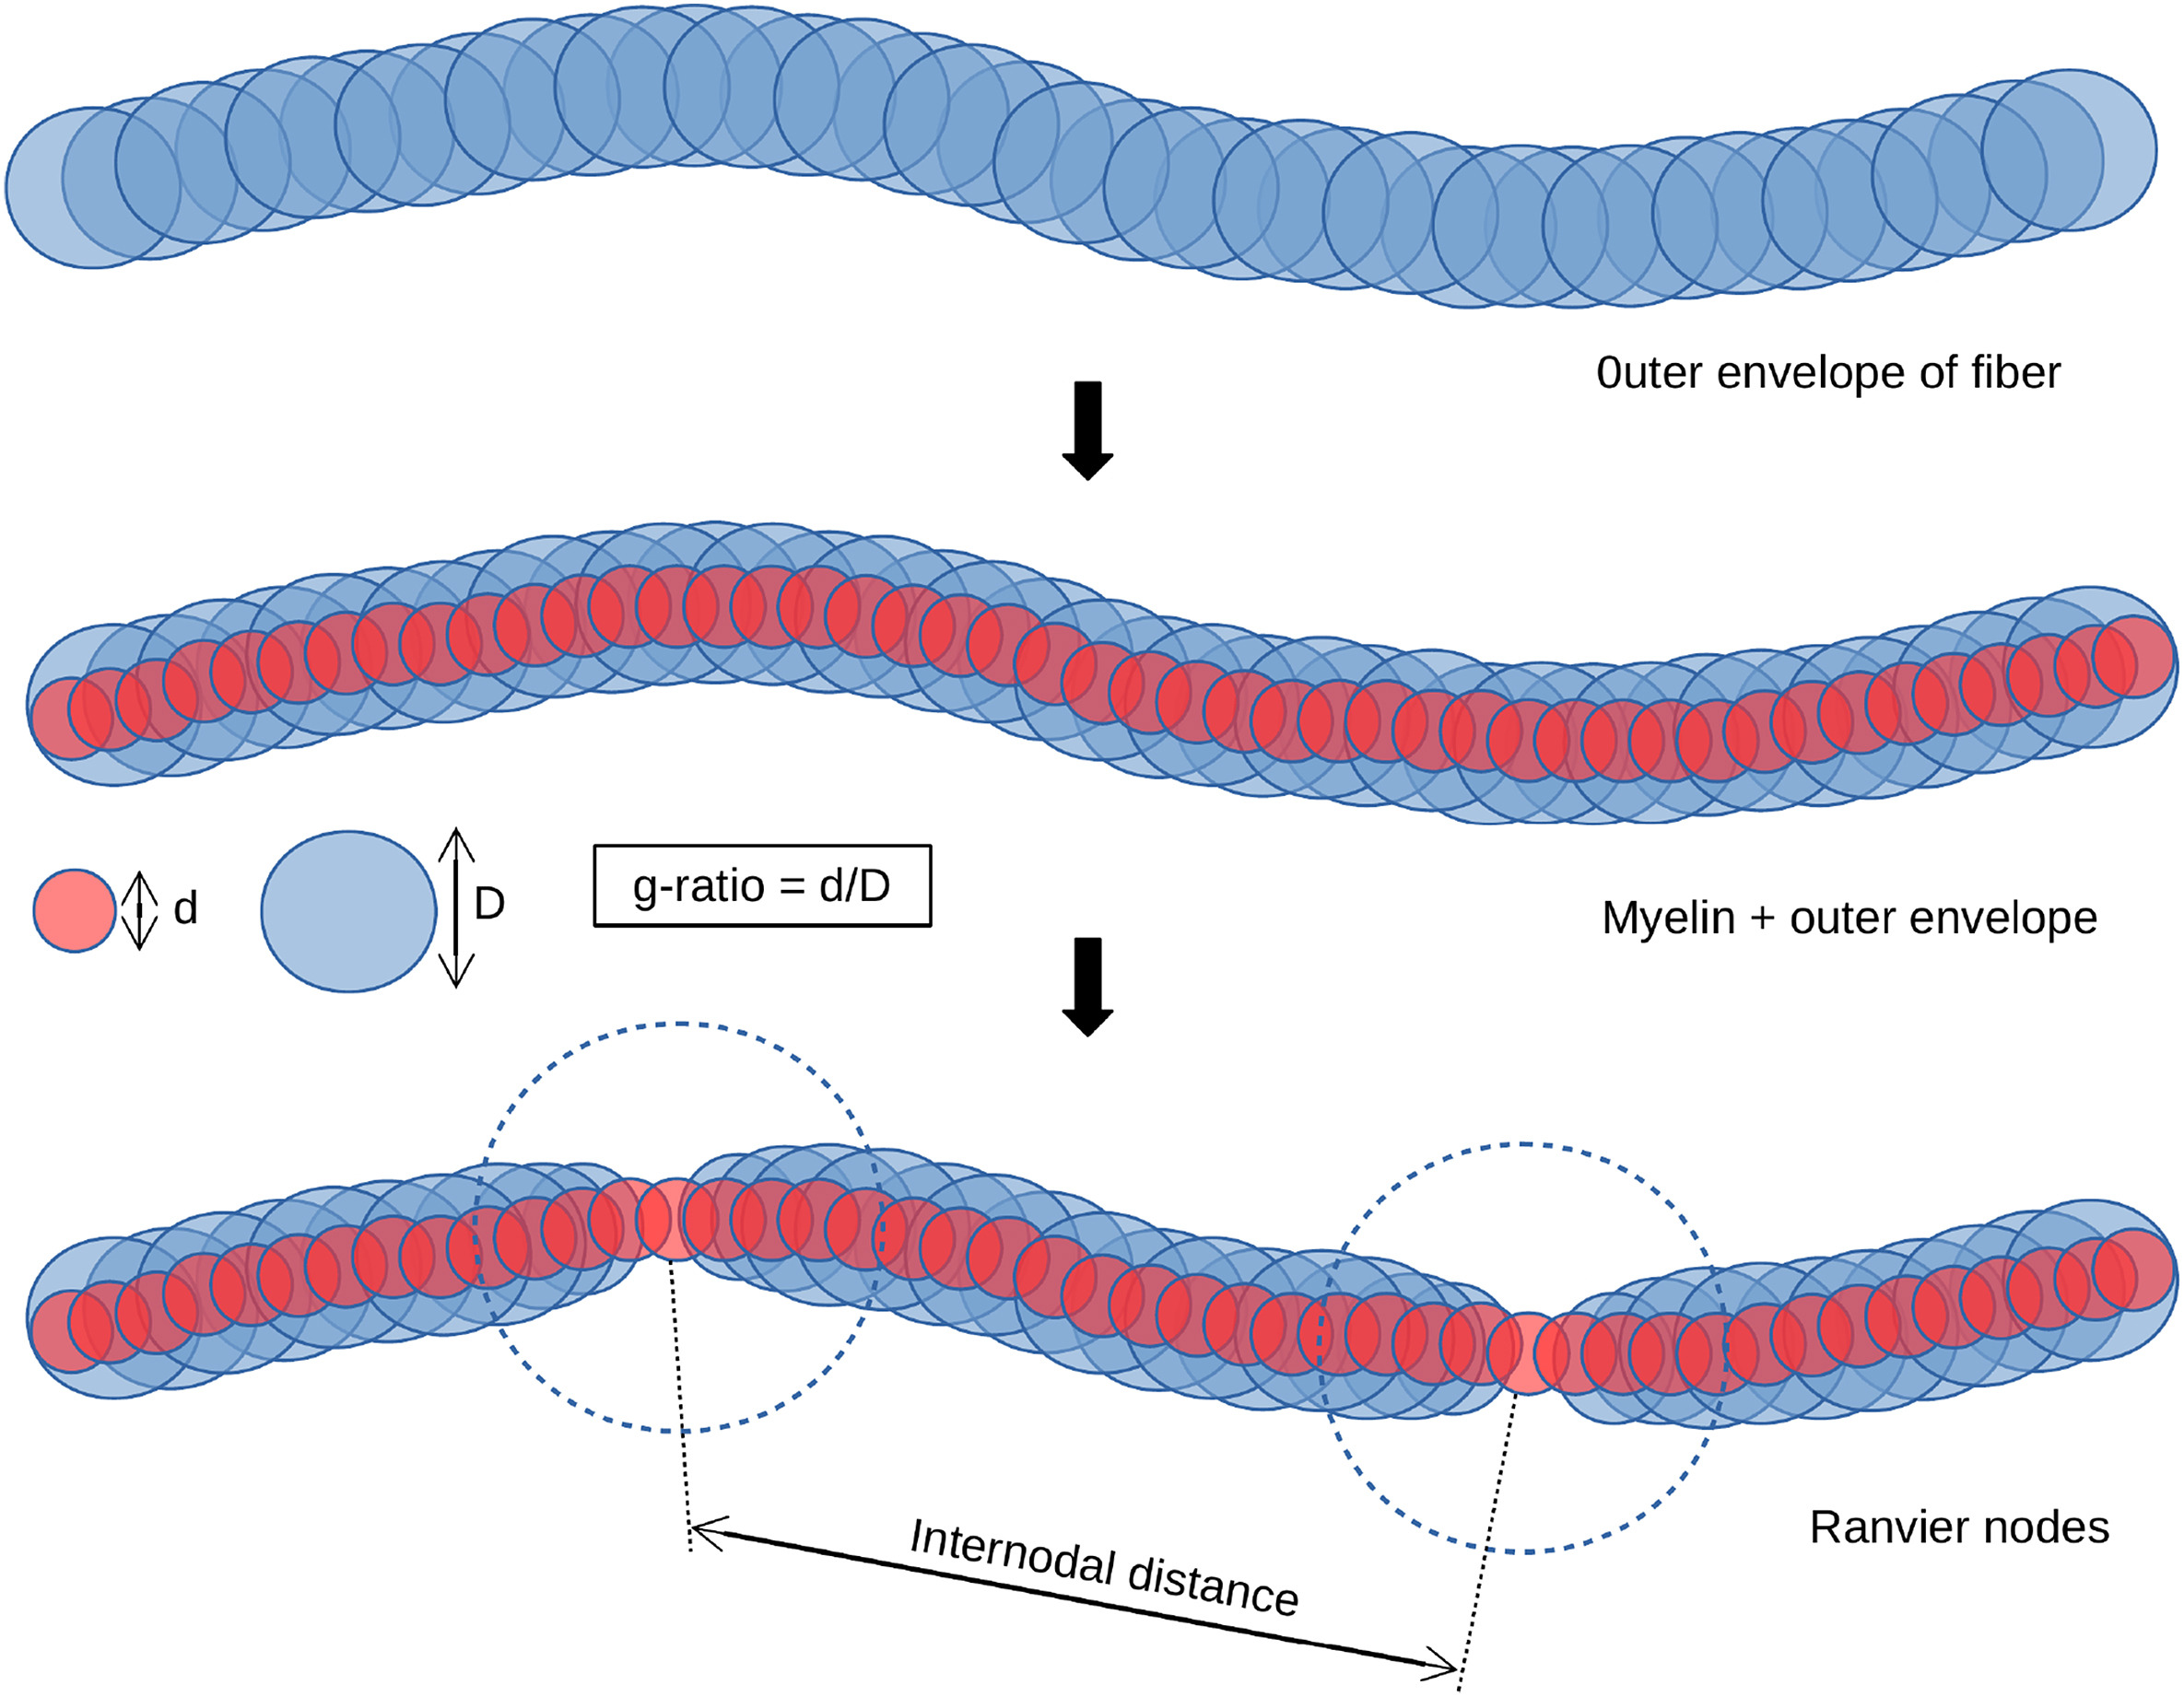
\includegraphics{gfx/model/medusa/4.jpg}
%     % }
% 	\caption{4 \cite{Ginsburger2019}}
% 	\label{fig:model:medusa_4_org}
% \end{figure}
% 
Since all objects are represented as a collection of spheres (see \cref{fig:model:medusa_4})
\begin{align}
    \mathcal{S} = \{ (x_i,y_i,z_i,r_i) : i \in \{0, 1, ..., n_\text{objects}-1\}  \} 
\end{align}
% 
, a collision is present if (VCS !!!)
% 
\begin{align}
\begin{split}
d<r_i+r_j\\
d = \abs{\vv{p}_i - \vv{p}_j}
\end{split}
\end{align}
% 
However since neighboring spheres in one fiber are colliding for a densly populated fiber, they have to be excluded if
\begin{align}
\begin{split}
d(i,j) &\leq  r_i + r_j\\
d(i,j) &= 
\begin{cases}
\sum_{n=i}^{j-1} \abs{\vv{p}_n - \vv{p}_{n+1}},& \text{if } j-i \geq 1\\
0 & \text{otherwise}
\end{cases}
\end{split}
\end{align}
% 
Spheres inside cell bodys are not checked for collision, since their volume aproximate? the volume of the cell.\\
% 
The calculation of collisions is done via the GPU architecture. For this a first implementation was written with the \textit{AxisAligedSortedSearch} \cite{Karras2012}. It sorteds the spheres along one axis, \eg x-axis, and search for each sphere the fist and last possible collision on this axis:
\begin{align}
\begin{split}
\mathcal{C}_i = \{ s \in \mathcal{S} \mid \abs{s_i.x - s_j.x} < r_i+r_j \}
\end{split}
\end{align}
% 
\begin{lstfloat}[!t]
	\lstinputlisting[style=cpp]{code/medusa.cu}
	\caption{Pseudocode of \acs{MEDUSA} collision checking.}
	\label{alg:medusa_collision}
\end{lstfloat}
% 
The above described algorithm is currently used for volumes $\approx \SI{200}{\micro\meter}$. For this volume size the algorithm is for the current use fast enough. However, more advaned algorithm exist wich can be applied here (\eg \textit{BoundindBoxHierarchy} \cite{Karras2012}).
% 
\subsection{Results}
% 
\begin{figure}[!t]
    \centering
    \resizebox{0.95\textwidth}{!}{
    \includegraphics{gfx/model/medusa/8.jpg}}
	\caption{8 \cite{Ginsburger2019}}
	\label{fig:medusa_8}
\end{figure}
% 
\begin{figure}[!t]
    \centering
    \resizebox{0.95\textwidth}{!}{
    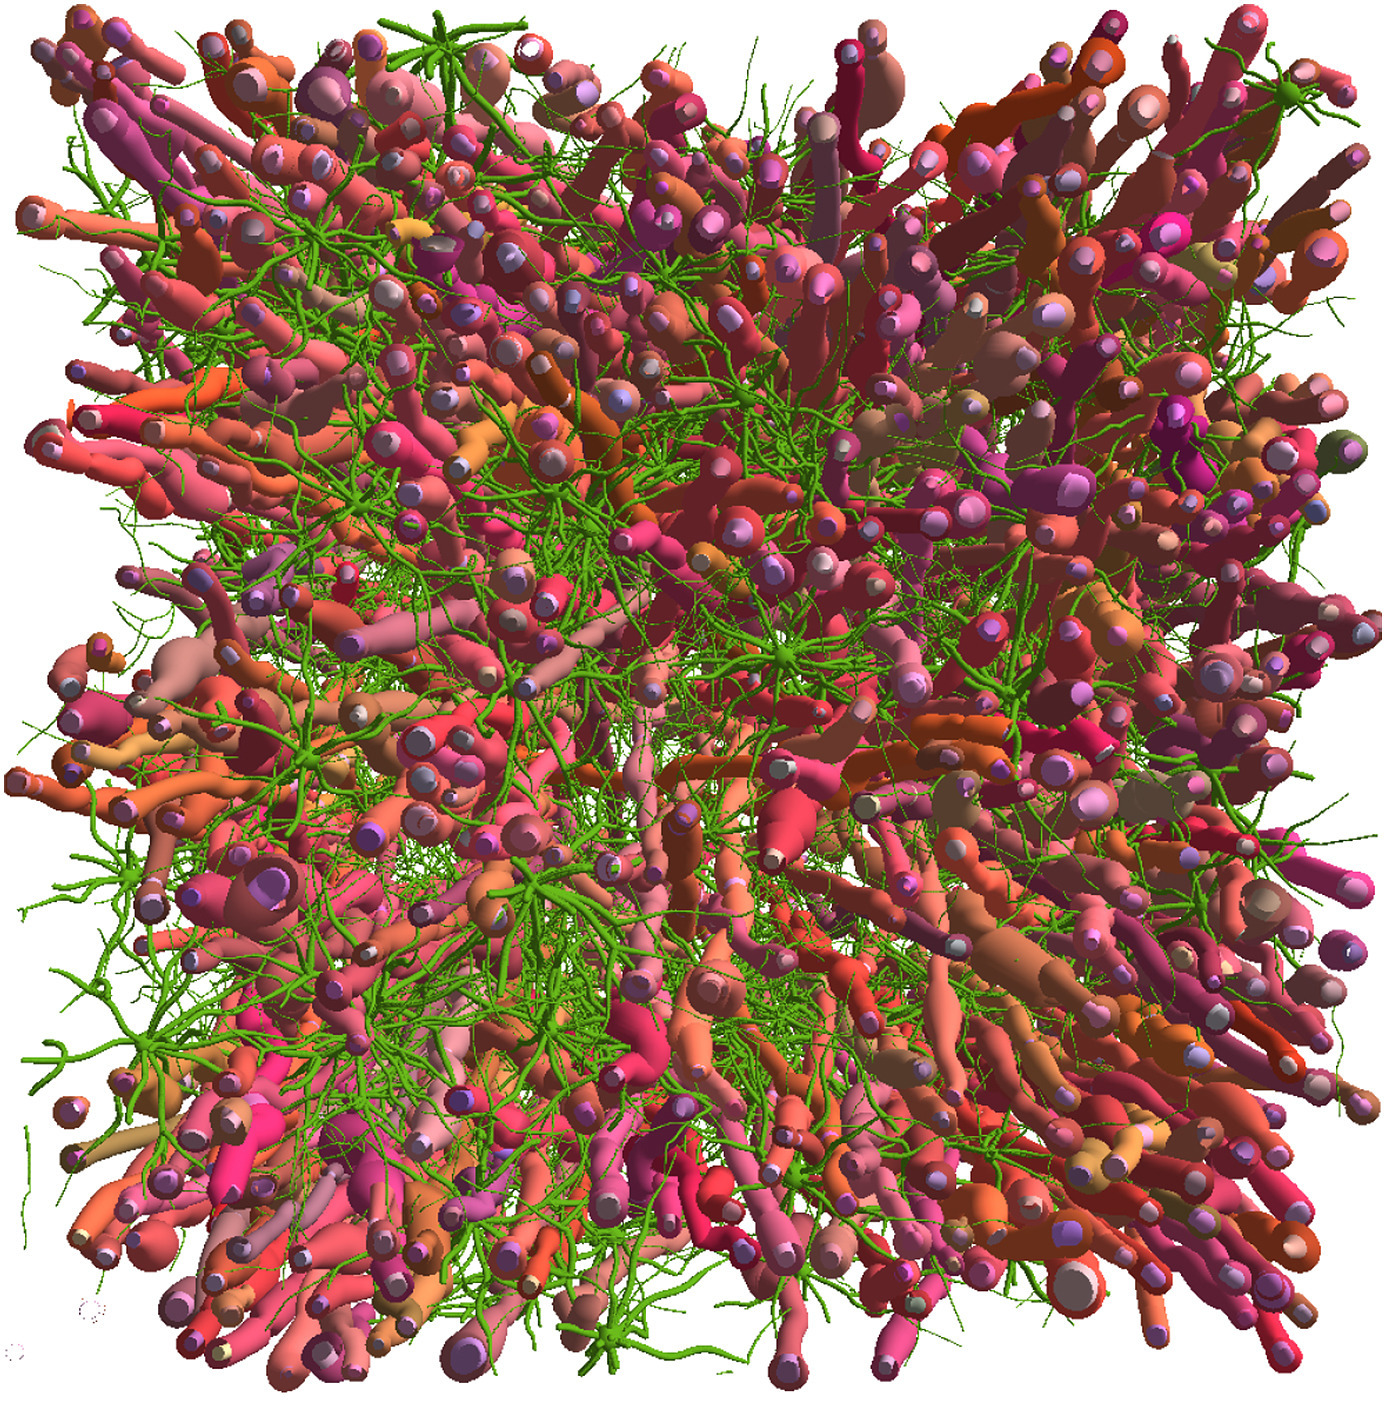
\includegraphics{gfx/model/medusa/11_.jpg}}
	\caption{11 \cite{Ginsburger2019}}
	\label{fig:medusa_11}
\end{figure}
% 
% 
% 
% 
% 
% 
% 
%
% Neurospin works with \ac{dMRI} signals.
% One focus is on the analysis of the fiber architect of the human brain.
% \ac{dMRI} is here quite handy since it is currently the only technique to allow in-vivo measurements to analyse the orientation of white matter tracts. Another importance is the availability of \ac{MRI} machines in almost every hospital in the western civilization.
% Although their resolution is with \SIrange{1.5}{3}{\tesla} limited.
% However, Neurospin is equipped with a mordern \SI{7}{\tesla} \ac{MRI}.
% This makes it possible, including higher measurments times on post mortem brain tissue, a \ac{dMRI} resolution up to \SI{200}{\micro\meter}.
% This makes it possible to allow \ac{3D-PLI} to verify and enhance the analysis of current developed tractography data. 
% %
% Along this works they developed a simulation tool (name) which is computing a Monte-Carlo simulation on the diffusion process in virtual tissues.
% Therefore, for simulations of the \ac{dMRI} signal in the brain, geometric models of nerve fibers as well as nerve cells are required.
% %
% The common goal was, due to a work packes inside the \ac{HBP}, the development of a common general purpose tool to build a geometrical library of nerve fiber configurations.
% Therefore it was decided to work based on the first approaches \cite{Ginsburger2018}.
% %
% \begin{quotation}
% We design a novel white matter numerical phantom generation algorithm which constructs biomimicking geometric configurations with few design parameters, and enables to control the level of disorder of the generated phantoms. The influence of various geometrical parameters present in white matter, such as global angular dispersion, tortuosity, presence of Ranvier nodes, beading, ...
% \end{quotation}
% %
% It is therefore qualified to generate a large database or library of parameter controlled white matter volumes.
% %
% \paragraph{differences:} 
% \begin{itemize}
%     \item All objects are aproximated with spheres.
%     \item Statistical ... of tissue
%     \item diffusion specific parameters
%     \item pathological changes like axon beeding
% \end{itemize}

% 
\cleardoublepage
\cleardoublepage
\setcounter{chapter}{5}
\chapter{\acs{3D-PLI} simulation}
\label{cha:sof:simulation}
%
Simulations of \ac{3D-PLI} have been used to study multiple effects of the microscopic technique involved with brain sections \cite{Dohmen2015,Menzel2015,Menzel2016,Menzel2020,Menzel2021,MenzelMaster,MenzelDissertation}.
The algorithm presented here for designing new collision-free fiber models allowed for the first time to simulate the effect of scattering light in light wave simulations base on finite-difference time domain agorithm without superimposed interference signals.
This enabled the understanding of scattering effects due to fiber bundle and crossing configurations as well as the transmission change for tilted fiber configurations \cite{MenzelDissertation,Menzel2020,Menzel2021}.
\par
% 
In the case of linear optics simulation, the optical system could be successfully simulated and the experimental results could be reproduced \cite{Dohmen2015,Menzel2016}.
The algorithm developed at that time is very computationally intensive and also very memory intensive due to the precomputations of a discretized tissue volume.
The foundations for a more efficient parallel algorithm for supercomputer architecture use were developed in response \cite{Lucksch2016}.
The new tilt design of the LMP3D microscope led to an unnecessary duplication of calculations in the simulations, which could not be easily changed in the algorithm designed at that time.
Therefore, the algorithm was redesigned from scratch.
Additionally, the fiber models presented here had to be incorporated as well.
Finally, the decision was made to switch to the M\"{u}ller-Stokes calculation in order to also take polarization effects of filters into account.
\par
%
The \ac{3D-PLI} simulation is divided into two consecutive parts: the discrete volume generator and the light matter simulation.
The discrete volume generator discretizes the virtual nerve fiber models onto a cartesian grid, which is then used to compute the light-matter interaction in the second step.
A parallelization technique with \ac{MPI} allows the volume to be partitioned among different \acp{CPU} or compute nodes.
Due to the tilting approach, the light vector in such a parallelized volume must be able to leave the current volume of a single \ac{CPU} and traverse to the next volume/process.
The computationally intensive algorithms are written in \cpp{} with an additionally user-friendly designed wrapper function in \python{}.
%
% 
% 
\section{Discrete volume generator}
\label{sec:dv_generator}
%
\begin{figure}[!t]
\centering
\setlength{\tikzwidth}{0.5\textwidth}
\inputtikz{gfx/simpli/disc_volume}
\caption{Discretized tissue volume with a voxel size \voxelsize. The volume is defined by a \ac{AABB}, which itself is defined by two points $\vec{v}_\mathit{min}$ and $\vec{v}_\mathit{max}$.}
\label{fig:discVol}
\end{figure}
%
The \ac{3D-PLI} simulation is to divide the necessary calculations into two consecutive parts. The first part is the calculation of a discretized tissue volume.
It represents a discrete, voxel model of the tissue.
This helps to drastically speed up the light-matter interaction of the next step (see \cref{sec:simulation}), at the cost of a large memory requirement.
\par
%
The discretized tissue volume represents a cuboid divided into smaller cubes of equal size, called voxels, \ie{} 3d pixels (see \cref{fig:discVol}).
Each voxel contains the physical properties absorption, birefringence and optical axis orientation of the tissue at its current position.
The total volume is bounded by a \ac{AABB} or \ac{VOI} defined by a minimum and maximum value $\voi = [(x_{\mathit{min}}, y_{\mathit{min}}, z_{\mathit{min}}), (x_{\mathit{max}}, y_{\mathit{max}}, z_{\mathit{max}})]$.
Additionally, the parameter \Voxelsize{} \voxelsize{} is set to a floating point number and defines the edge length of the equilateral voxels.
If the division of any of the \voi{} axis by \voxelsize{} is not an integer, the corresponding axis of the \voi{} is incremented to the nearest possible integer value to avoid edge effects.
%
%
%
\subsection{Nerve fiber layers}
%
As described in \cref{sec:fiberArchitecture}, nerve fibers are axons that can be wrapped by multiple turns of myelin (see \cref{fig:myelinLayer}).
Especially for light wave simulations, the myelin windings are an important feature \cite{MenzelDissertation}.
\par
%
The windings are represented as individual layers (see \cref{fig:fiberLayer}).
This greatly simplifies the creation process.
A layer is defined by a factor between $\SI{0}{}$ and $\SI{1}{}$ that scales with the radius of the nerve fiber.
For example, $\SI{0.75}{}$ means that from $0 \leq r < 0.75$ of the radii is interpreted as the first layer (see \cref{fig:fiberLayer}).
\par
%
Each layer requires a number of physical properties in addition to its radius:
%
\begin{itemize}[nosep]
    \item birefringence value: $\dn$
    \item absorption coefficient: $\mu$
    \item optical axsis model: $p=\mathit{parallel}$, $r=\mathit{radial}$, $b=\mathit{background}$
\end{itemize}
%
These properties are specified as a list of tuples within the algorithm (see \cref{alg:fiberbundleprops}).
%
%
At the end, the discretize volume generator returns the arrays \tissue{}, \opticalaxis{} and \propertylist{} for use in the light matter simulation.
Since the arrays are quite large, the transfer is performed as a ownership movemend of a \name{numpy-array} without having to copy the data.
% 
\begin{lstfloat}[!ht]
\lstset{style=python}
\begin{lstlisting}[]
fbs_properties = [[(r, dn, mu, 'p'), (second layer), ...],
                  [(first layer of second bundle), ...],
                  [...]]
\end{lstlisting}
\caption{Definition of the properties of fiber bundles.}
\label{alg:fiberbundleprops}
\end{lstfloat}
% 
% 
% 
\subsection{Discretization of a nerve fiber model}
%
\begin{figure}[!t]
\centering
\setlength{\tikzwidth}{0.3\textwidth}
\subcaptionbox{\label{fig:myelinLayer}Schematic representation of a nerve fiber with axon and myelin sheath}
[\tikzwidth]{\includegraphics[height=\tikzwidth]{dev/brain/myelin_layers.pdf}\vspace{0mm}}\hfill
\subcaptionbox{\label{fig:fiberLayer}Cross section through a nerve fiber with layered structure defined by $n$ radii}
[\tikzwidth]{\inputtikz{gfx/simpli/fiber_layer}\vspace{-5mm}}\hfill
\subcaptionbox{\label{fig:vectormodel}Cross section of a discretized nerve fiber with resulting optical axis vectors}
[\tikzwidth]{\inputtikz{gfx/simpli/vector_model}\vspace{-5mm}}
\caption{Discretization of nerve fibers with layered structure.}
\label{fig:fiber_discretization}
\end{figure}
%
To discretize nerve fiber models individual nerve fiber segment are discretized after each other, since a fiber is a chain of consecutive segments.
Each voxel inside a fiber segment has to be labled as a tissue with the physical properties at the voxel center position $\vec{q}$ (see \cref{fig:fiber_discretization}).
The discretized mesh represents an array, where an element at position $[i,j,k]$ occupies the space from $(i,j,k)$ to $(i+1,j+1,k+1)$ in the unit of $\SI{1}{\voxelsize}$.
\par
%
To identify all voxels inside a volume all voxels inside the fiber segments are checked if they are inside the fiber segment.
Therefore a loop over all voxels is performed.
\par
%
To calculate if a voxels is inside the nerve fiber segment,
a computation analogously to the collision between two nerve fiber segments is calculated (see \cref{alg:pseudocodeCollisionDetection}).
The difference is, that only one point on a the fiber segment line has to be calculated.
The second point is the voxels center $\vec{q}$.
From this calculation, not only the nearest points $\vec{p}_a$ and $\vec{p}_b$ are returned, but also the distance vector $\vec{d}$.
The distance of the vector is used to check whether the voxel is inside the fiber segment, and if so, in which layer of the fiber segment it is located.
if the optical axis orientation follows a macroscopic model, the points $\vec{p}_a, \vec{p}_b$ are used to calculate the orientation.
\par
%
In case of a voxel occupied by a fiber segment, two values are stored.
The first one is an index within an array \name{tissue} which will be used later to retrieve the properties from a list with the same index order.
The second information is the orientation of the optical axis within the current layer, stored in the array \name{optical\_axis}.
The orientation is either parallel to the fiber segment in the case of the macroscopic model, or radial in the case of the microscopic model.
A layer can also be marked as \say{background}, allowing the user to specify an area without any birefringence.
\par
%
The next step is to loop aver all fiber segments and fill the volume.
However, another problem must be solved first.
Since two consecutive fiber segments occupy the same space because they have a common point, they also fill some voxels of the tissue volume simultaneously.
This is a problem because the processed second fiber segment overwrites the values of the first.
This is solved by using an additional array that stores the smallest distance calculated when filling the voxels space.
The values are only overwritten when a new distance is calculated that is smaller than the one already stored.
This solves also the problem that in a radial optical axis model, the optical axis is star-shaped at the end points of each fiber segment inside the fiber.
The first and last point of a fiber, however, are not affected by this.
\par
%
The algorithm for the discretization loop is shown in \cref{alg:fillVolume}.
%
\begin{lstfloat}[!tb]
\lstset{style=python}
\begin{lstlisting}[]
for fiber_segment in fiber_bundle:
    for i,j,k in fiber_segment.aabb().voxels():
        min_dist, min_point = calculate_min_distance((i,j,k), cc)
        if min_dist < cc.radius:
            if min_dist < current_distance[i,j,k]:
                optical_axis[i,j,k,:] = get_axis_orientation(
                                            (i,j,k), min_dist,
                                            min_point)
                tissue[i,j,k] = get_layer_id(min_dist)
                current_distance[i,j,k] = min_dist
\end{lstlisting}
\caption{Pseudocode for filling the discretized volume.}
\label{alg:fillVolume}
\end{lstfloat}
%
\paragraph{Additional Information}
Since the light matter simulation algorithm recieves an \name{tissue}, \name{optical\_axis} and \name{propertie} array, the user can also change the values in between both algorithms.
In the upper algorithm, the optical axis vectors length is $\SI{1}{}$.
The length of the vector is in the light matter simulation part interpreted as the birefringence strength factor.
Therefore the user can \eg{} add additionall variability of the strength of the birefringence.
%
%
%
\subsection{\Voxelsize}
%
\begin{figure}[!t]
\centering
% \tikzset{external/export=false}
\setlength{\tikzwidth}{.24\textwidth}
\definecolor{c1}{rgb}{0.25,0.4,0.1}
\definecolor{c2}{rgb}{1.0,0.73,0}
\definecolor{c3}{rgb}{0.98,0.4,0.25}
\definecolor{c4}{rgb}{0.22,0.36,0.59}
%
% \definecolor{c1}{HTML}{440154FF}
% \definecolor{c2}{HTML}{38598CFF}
% \definecolor{c3}{HTML}{1E9B8AFF}
% \definecolor{c4}{HTML}{FDE725FF}
%
\def\xc{0.7}
\def\yc{0.2}
\def\rin{1.5}
\def\rout{3}
%
% 
\newcommand{\fiber}[3]{
	\def\dd{#1}
	\pgfmathsetmacro{\xmin}{int(floor(\xc-\rout))}
	\pgfmathsetmacro{\xmax}{int(ceil(\xc+\rout))}
	\pgfmathsetmacro{\xd}{\xmin+\dd}
	\pgfmathsetmacro{\ymin}{int(floor(\yc-\rout))}
	\pgfmathsetmacro{\ymax}{int(ceil(\yc+\rout))}
	\pgfmathsetmacro{\yd}{\ymin+\dd}
	%
	\pgfmathsetmacro{\rmin}{\rin*\rin*100}
	\pgfmathsetmacro{\rmax}{\rout*\rout*100}
	\foreach \x in {\xmin,\xd,...,\xmax} {
		\foreach \y in {\ymin,\yd,...,\ymax} {
			\pgfmathsetmacro{\d}{int(((\x-\xc+\dd/2)*(\x-\xc+\dd/2)+(\y-\yc+\dd/2)*(\y-\yc+\dd/2))*100)}
			\ifnum\d>\rmin
			\ifnum\d<\rmax
			\path [#3] (\x,\y) rectangle ($ (\x, \y) + (\dd, \dd) $);
			\draw[#2] ($ (\x, \y) + (0, 0) $) -- ($ (\x, \y) + (\dd, 0) $);
			\draw[#2] ($ (\x, \y) + (\dd, 0) $) -- ($ (\x, \y) + (\dd, \dd) $);
			\draw[#2] ($ (\x, \y) + (\dd, \dd) $) -- ($ (\x, \y) + (0, \dd) $);
			\draw[#2] ($ (\x, \y) + (0, \dd) $) -- ($ (\x, \y) + (0, 0) $);
			\fi\fi
		}
	}
%	\foreach \x in {\xmin,\xd,...,\xmax} {
%		\draw[#2] (\x,\ymin) -- (\x,\ymax);
%	}
%	\foreach \y in {\ymin,\yd,...,\ymax} {
%		\draw[#2] (\xmin,\y) -- (\xmax,\y);
%	}
}
%
\subcaptionbox{}[\tikzwidth]{
\resizebox{\tikzwidth}{!}{
\begin{tikzpicture}[]
\path[] (-3.75, -3.5) rectangle (3.75, 3.25);
\begin{scope}[shift={(-\xc,-\yc)}]
\fiber{2}{line width = 0.2mm}{pattern color=c1,pattern=horizontal lines}
\draw[line width = 0.4mm] (\xc,\yc) circle (\rin);
\draw[line width = 0.4mm] (\xc,\yc) circle (\rout);
\end{scope}
\end{tikzpicture}
}}
\hfill
%
\subcaptionbox{}[\tikzwidth]{
\resizebox{\tikzwidth}{!}{
\begin{tikzpicture}[]
\path[] (-3.75, -3.5) rectangle (3.75, 3.25);
\begin{scope}[shift={(-\xc,-\yc)}]
\fiber{1}{line width = 0.1mm}{pattern color=c2,pattern=vertical lines}
\draw[line width = 0.4mm] (\xc,\yc) circle (\rin);
\draw[line width = 0.4mm] (\xc,\yc) circle (\rout);
\end{scope}
\end{tikzpicture}
}}
\hfill
%
\subcaptionbox{}[\tikzwidth]{
\resizebox{\tikzwidth}{!}{
\begin{tikzpicture}[]
\path[] (-3.75, -3.5) rectangle (3.75, 3.25);
\begin{scope}[shift={(-\xc,-\yc)}]
\fiber{0.5}{line width = 0.05mm}{pattern color=c3,pattern=north east lines}
\draw[line width = 0.4mm] (\xc,\yc) circle (\rin);
\draw[line width = 0.4mm] (\xc,\yc) circle (\rout);
\end{scope}
\end{tikzpicture}
}}
\hfill
%
\subcaptionbox{}[\tikzwidth]{
\resizebox{\tikzwidth}{!}{
\begin{tikzpicture}[]
\path[] (-3.75, -3.5) rectangle (3.75, 3.25);
\begin{scope}[shift={(-\xc,-\yc)}]
\fiber{0.25}{line width = 0.025mm}{pattern color=c4,pattern=crosshatch dots}
\draw[line width = 0.4mm] (\xc,\yc) circle (\rin);
\draw[line width = 0.4mm] (\xc,\yc) circle (\rout);
\end{scope}
% \fiber{2}{}{fill, c1, opacity=0.25}
% \fiber{1}{very thin}{fill, c2, opacity=0.25}
% \fiber{0.5}{ultra thin}{fill, c3, opacity=0.25}
% \fiber{0.25}{ultra thin}{fill, c4, opacity=0.25}
%
\end{tikzpicture}
}}
\caption{Discretization error. Cross-section through a single fiber with a myelin layer in the discretized tissue volume. The colored pattern shows the resulting voxels corresponding to the fiber. The smaller the \Voxelsize, the smaller the discretization error.}
\label{fig:vectorfield_disc_error}
\end{figure}
%
The parameter \Voxelsize{} is a very important property of the light matter simulation.
It determines how accurate the volume is represented (see \cref{fig:vectorfield_disc_error}).
Additionally the in the light matter simulation one light ray is casted from each voxel of the bottom plane (see \cref{sec:pathOfLight}). 
Therefore it is also responisble for the sampling of the resulting intensities.
%
%
% 
\subsection{Optimizations}\label{sec:dvOpti}
%
All arrays are implemented as contiguous c-arrays, accessible externally as \name{numpy-arrays} without the need to copy the data.
Since these arrays grow with $\mathcal{O}(\frac{1}{\voxelsize}^3)$, the ownership of the data is movable in both the \cpp{} libraries and \python{} code.
The memory order of the arrays is in the $x\text{-}y\text{-}z$ direction, so the largest memory shift is in $x$ and the smallest in $z$.
This was chosen so that later in the light matter simulation part, where the light moves mainly in the $z$-direction, the memory is aligned with the traversed information and thus the \acp{CPU} cache prefetcher can be used effectively.
\par
%
Two methods are used to parallelize the algorithm on the \ac{CPU}.
The first uses \ac{OpenMP} to parallelize the filling of the \ac{AABB} volume of each object.
The second uses \ac{MPI} to allow distribution across multiple \ac{CPU} cores without sharing memory (detailed description in \cref{sec:mpiSim}).
\par
%
Parallelizing the filling prozess of the voxels of the discretized volume leads to a race condition when multiple threads want to write or read to the same memory address, \ie{} the same coordinate in the volume.
A solution with a lock would be very slow and since many of the voxels do not need to be overwritten, most of the locks would be unnecessary.
To share the work, thread $n$ processes only the memory for the first index $i$ (or volume dimension $x$) if:
%
\begin{align}
\begin{split}
    i \bmod N_{\mathit{Threads}} == \mathit{thread}_{\mathit{id}}
\end{split}
\end{align}
%
\begin{figure}[!t]
\centering
\setlength{\tikzwidth}{0.5\textwidth}
\inputtikz{gfx/simpli/disc_volume_thread}
\caption{Discretization volume parallelization with \ac{OpenMP}. Each thread processes every $n$-th $yz$-section. This ensures both thread safety and a more balanced workload, even under inhomogeneous conditions.}
\label{fig:discVolThread}
\end{figure}
% 
This means that each thread loops over every $N_{\mathit{num\_threads}}$ slice of the volume (see \cref{fig:discVolThread}).
This is done instead of dividing the volume to n sub volumes to distribute the work in case that the volume is not filled homogeniously with fibers.
This procedure leads to a thread-safe writable operation.
One disatvantage of this algorithm is, that all threads have to check if the \ac{AABB} of all fiber segments is inside the current \ac{VOI}.
% 
% 
%
\section{Light matter Simulation}
\label{sec:simulation}
%
The light matter simulation algorithm performs the Mueller-Stokes calculation (see \cref{sec:Mueller-Stokes}) on the previously calculated discrete volume (see \cref{sec:dv_generator}) for the light rays along their paths.
Since no scattering or refraction effects are considered in this simulation, each light path follows a straight line.
Initially, the light vector is multiplied by the first polarizer of the optical system (see \cref{sec:expSetup}).
The path inside the tissue is discretized into steps.
The interaction between the light ray and the tissue is calculated after each step according to $ \vec{S}' = \prod_i \left(\mat{R}_i \mat{M}_i \mat{R}_i\right) \cdot \vec{S}$ (see \cref{sec:mueller_stokes, sec:simLightTissue}).
% After a light beam reaches the end of the tissue, the last optical elements of the setup are applied to the lights vector.
% Finally, the light intensity is stored in the \acs{CCD} image array, which at this point of the algorithm has the same size as the 2d $xy$ grid of the discretized tissue.
% In a later step, the intensities will be blurred and resampled to the acually \ac{CCD} pixels size and noise will we added according to the users specifications.
% 
%
%
\subsection{Light ray path}
\label{sec:pathOfLight}
%
\begin{figure}[!t]
\setlength{\tikzheight}{0.42\textwidth}
\subcaptionbox{camera view}
[.475\textwidth]{\inputtikz{gfx/simpli/tilting_3d_a}}\hfill
\subcaptionbox{perspective view}
[.475\textwidth]{\inputtikz{gfx/simpli/tilting_3d_b}}
\tikzset{external/export=false}
\caption[3d tilting]{3d tilting: around $xy$-axis, \raisebox{.25em}{\tikz \draw[red,thick](0,0)--(0.25,0);} top, \raisebox{.25em}{\tikz \draw[green,thick](0,0)--(0.25,0);} middle, \raisebox{.25em}{\tikz \draw[blue,thick](0,0)--(0.25,0);} bottom, \raisebox{.25em}{\tikz \draw[dash pattern=on 1.25pt off 1.25pt,thick](0,0)--(0.25,0);} original, \raisebox{.25em}{\tikz \draw[gray](0,0)--(0.25,0);} axis of rotation.}
\label{fig:tilting_camera_view}
\end{figure}
%
The light matter simulation allows for a tilting light beam.
For this purpose, the \ac{LAP} uses a tilting stage to which the tissue sections are attached (see \cref{fig:tilting_camera_view}).
The \ac{LMP3D}, on the other hand, has an tilted light beam.
This is achieved by a conical light path, from which an aperture is then used to sample the desired light direction \cite{Wiese:887678}.
Both methods can be mathematically represented by the same procedure.
\par
%
An additional effect changing the light path is the refraction at the tissue-air boundary, which is described by Snell's law for isotropic media (see \cref{eq:Snellius}).
Since this only adds a parallel shift, simulation is only necessary when the effects of the resampling process and image registration is to be investigated.
\par
%
\begin{figure}[!t]
\setlength{\tikzwidth}{0.45\textwidth}
\subcaptionbox{normal}[.475\textwidth]{
\def\tilt{0}
\def\nindex{2.25}
\inputtikz{gfx/simpli/tilting_a}}\hfill
\subcaptionbox{tilted}[.475\textwidth]{
\inputtikz{gfx/simpli/tilting_b}}
\caption[Light path]{Light ray path for a normal (a) and a tilted (b) case. In the tilted case, the light beam $\vec{l}_1$ is tilted within the tissue and thus experiences an optical shift $\Delta$.}
\label{fig:tilted_side_view}
\end{figure}
%
The initial position of the light beam is calculated by traversing the light path backwards (see \cref{fig:tilted_side_view}).
This has the advantage, that the each index inside the \ac{CCD} receives always exactly one light beam.

From the \ac{CCD} array, the light path can be shifted back to the top plane of the tissue $\mathfrak{S}_{top}$.
Subsequently, the light beam $\vec{l}_1$ is traced back through the tissue to the bottom plane $\mathfrak{S}_{bottom}$.
The point on the lower tissue plane corresponds to the initial position of the light beam.
This light path change results in a shift $\delta$ along the same direction of the tilting.
In the light matter simulation only light rays are considered, which will go at least partially through the volume.
All remaining \ac{CCD} elements are left with a \textit{NaN} value.
\par
%
The tilting of the tissue leads to a distortion of the image (see \cref{fig:tilting_camera_view}).
This distortion can be described by an affine transformation (see \cref{fig::affine_transformation}):
%
\begin{figure}[!t]
\centering
\pgfmathsetmacro{\size}{10}
% 
\subcaptionbox{}[.225\textwidth]{
\resizebox{.225\textwidth}{!}{
\begin{tikzpicture}[]
\pgfmathsetmacro{\dx}{2.25}
\pgfmathsetmacro{\dy}{1.5}
\draw[help lines] (0,0) grid (\size,\size);
\foreach \i in {0,...,\size}{
	\draw [very thick] (\i+\dx, 0+\dy) -- (\i+\dx, \size+\dy);
	\draw [very thick] (0+\dx, \i+\dy) -- (\size+\dx, \i+\dy);
}
\end{tikzpicture}
}}
% 
\subcaptionbox{}[.225\textwidth]{
\resizebox{.225\textwidth}{!}{
\begin{tikzpicture}[]
\pgfmathsetmacro{\sx}{1.5}
\pgfmathsetmacro{\sy}{0.75}
\draw[help lines] (0,0) grid (\size,\size);
\foreach \i in {0,...,\size}{
	\draw [very thick] ({\i*\sx}, 0) -- ({\i*\sx}, {\size*\sy});
	\draw [very thick] (0, {\i*\sy}) -- ({\size*\sx}, {\i*\sy});
}
\end{tikzpicture}
}}
%
\subcaptionbox{}[.225\textwidth]{
\resizebox{.225\textwidth}{!}{
\begin{tikzpicture}[]
\draw[help lines] (0,0) grid (\size,\size);
\begin{scope}[rotate around={30:(0.5*\size,0.5*\size)}]
\foreach \i in {0,...,\size}{
	\draw [very thick] (\i, 0) -- (\i, \size);
	\draw [very thick] (0, \i) -- (\size, \i);
}
\end{scope}
\end{tikzpicture}
}}
% 
\subcaptionbox{}[.225\textwidth]{
\resizebox{.225\textwidth}{!}{
\begin{tikzpicture}[]
\pgfmathsetmacro{\cx}{0.5}
\pgfmathsetmacro{\cy}{0}
\draw[help lines] (0,0) grid (\size,\size);
\foreach \i in {0,...,\size}{
	\draw [very thick] (\i+0*\cx, 0+\i*\cy) -- (\i+\size*\cx, \size+\i*\cy);
	\draw [very thick] (0+\i*\cx, \i+0*\cy) -- (\size+\i*\cx, \i+\size*\cy);
}
\end{tikzpicture}
}}
\caption{affine transformation}
\label{fig::affine_transformation}
\end{figure}
%
\begin{align}
f(\vec{x}) = \mat{A} \cdot \vec{x} + \vec{t}
\end{align}
where $\vec{x}$ is the coordinate input, $\mat{A}$ and $\vec{t}$ are the transformation values, and $f(\vec{x}$ is the transformed coordinate.
\par
%
The light matter simulation with the light paths sampling as described above takes this distorted view into acount and removes it.
The simulation is also capable of sampling the light rays in such a way, that the distortion occurs.
In that case the resulting images have to be registered onto each other \eg{} by an affine transformation wich is also available.
% 
% 
% 
\subsection{Tissue voxel interpolation}
%
If the \Stepsize{} of the light ray is not equal to the \Voxelsize{} or if the light path is tilted, the light rays position after a step does not longer matches the center of the voxel.
This means that the physical properties stored in the arrays have to be interpolated.
%
\begin{figure}[!t]
\centering
\setlength{\tikzwidth}{0.475\textwidth}
% \tikzset{external/force remake=true}
\subcaptionbox{\label{fig:triInterp}Trilinear interpolation}
[\tikzwidth]{
\hfill\inputtikz{gfx/simpli/trilinear_interpolation}\hfill}\hfill
\subcaptionbox{\label{fig:sphInterp}Spherical interpolation}
[\tikzwidth]{
\inputtikz{gfx/simpli/vector_interpolation}}
\caption{Interpolation techniques: Trilinear interpolation can be represented as an axial step interpolation. The difference between linear and spherical interpolation is that linear interpolation has a constant distance $s$ between each point, while spherical interpolation has a constant angle $\varphi$ between two steps.}
\label{fig:vectorfield_disc}
\end{figure}
%
Currently three interpolation methods are implemented: \name{nearest neighbor}, \name{linear interpolation} and \name{spherical interpolation}.
The voxels considered for interpolation are the nearest eight neighboring voxels, i.e. array indices $(\floor{x\pm0.5},\floor{y\pm0.5},\floor{y\pm0.5})$.
The \name{nearest neighbor} and \name{linear interpolation} are still present from the development phase.
However, they should not be used because they are error-prone.
Since the data are orientations, the default value for the interpolation method \name{spherical interpolation} should be used.
%
%
%
\subsection{Simulation of light matter interaction}\label{sec:simLightTissue}
%
After the initial light positions are calculated each light beam is traversed within the tissue.
To calculate the light-tissue interaction, the change of the Stokes vector is calculated after each light beam step.
The step size is a user defined value with a default value of the \Voxelsize{} $\voxelsize$.
Once the light hits the boundary of the volume, the light beam is multiplied by the matrix of the remaining optical elements of the microscop and the intensity is stored in the \ac{CCD}-array.
The pseudocode is shown in \cref{alg:simulationLoop}.
%
\begin{lstfloat}[!tb]
\lstset{style=python}
\begin{lstlisting}[]
light_beams = calculate_light_starting_positions()

for light in light_beams:
    light = optical_elemts_start * light
    while light.pos in volume:
        properties = get_properties(light.pos)
        light.intensity *= exp(-step_size * properties.absorbtion)
        light = matrix(properties) * light
        light.pos += step_size
   
    light = optical_elemts_end * light
    ccd_array[light.ccd_pos] = light.intensity
\end{lstlisting}
\caption{Loop over the light vectors for the light-tissue interaction. Their intensity value is stored inside the \ac{CCD} array.}
\label{alg:simulationLoop}
\end{lstfloat}
%
To resample the array to the final size of the \ac{CCD} sensor and apply noise model python funcions exits outside of the parralized simulation software.
% 
% 
%
\subsection{Optimizations}
%
Several optimizations exists in this pipeline.
First, the order of the tissues stored in memory is along the z-axis (as described in \cref{sec:dvOpti}) so that the light ray \textit{traverses} along the aligned memory.
Second, the for-loop for the light beams (see \cref{alg:simulationLoop}) is paralellized with \ac{OpenMP}.
These threads are completely separated and there are no race conditions.
In addition, all vector and matrix calculations are optimized for their small sizes by the compiler with the help of tools like \name{Compiler Explorer}\footnote{\url{https://godbolt.org/}} and \name{C++ Insight}\footnote{\url{https://cppinsights.io/}}.
%
%
\section{Optical system and signal analysis}
\label{sec:ccdOptic}
%
The image sensor, as described in \cref{sec:expSetup}, is a \ac{CCD}-sensor.
The the resampling and noise modeling, are implemented according to \cref{sec:opticalResolution}.
These calculations are performed on the \python{} side of the algorithm (\code{fastpli.simulation.Simpli}) and can be executed with the \code{multiprocessing} library of \python{} to use multiple \ac{CPU} cores.
Therefore when using \ac{MPI} (see \cref{sec:mpiSim}) the intensity image has to be reduced to a single process.
Since this image is only two dimensional, there is no need to speed up the process with \ac{MPI} further.
\par
%
To analyse the signal, the same algorithms are implemented as in the \ac{3D-PLI} routine pipeline (see \cref{sec::intSignal,sec::InclAnalysis}).
This include the modalities analysis transmittance, direction and retardatation as well as the tilting analysis performend by \ac{ROFL}.
The tilting analysis takes quite a lot time.
Therefore it can also be executed with the \code{multiprocessing} library of \python{}.
%
%
%
\section{MPI parallelization}\label{sec:mpiSim}
%
Both algorithms, the discrete volume generator and the light matter simulation, can additionally use a parallelization technique.
For large volumes that are larger than the local memory size, the computation must be split among multiple physical \acp{CPU}s and \name{computation nodes}.
For this purpose, \acreset{MPI} \ac{MPI} is used.
A method is implemented to automatically partition the volume along the $x$-axis and the $y$-axis into blocks with minimal surface area along both axis (see \cref{fig:com_halo}).
\par
% 
Each \ac{CPU} can performed the discrete volume generation without the knowlege of each other.
The exception is the light matter simulation for tilted light beams.
Here, when a light ray leaves the local volume, it must be transmitted to the adjacent volume.
\ac{MPI} provides several methods to send information to another \name{rank}.
Since the subvolumes are splitted along a cartesion grid, the cartesion implementations of \ac{MPI} are used (\eg{} \code{MPI\tu Cart\tu create}).
%
\begin{figure}[!t]
    \centering
    \setlength{\tikzwidth}{0.85\textwidth}
    \inputtikz{gfx/simpli/com_halo}
    \caption{ This example uses six \ac{MPI} ranks to split the entire volume into six subvolumes. To calculate the value at a given point a eight-neighborhood is necessary. Therefore a \name{halo} area (coloured voxels) with the same information shared by neighboring \ac{MPI} process is necesarry.}
    \label{fig:com_halo}
\end{figure}
%
A problem is the calculation at the edge of the volume, because the light beam needs the information of the surrounding eight voxels for the interpolation.
If this voxel information were to be transmitted to the neighboring \name{rank} as well, this would mean a large amount of communication, which is much slower compared to the local \ac{CPU} or \ac{RAM} instructions.
The solution is a so-called \name{halo}.
This is a commonly used concept where the boundaries (in this case a volume) are increased by a certain size (in this case $\SI{1}{\voxel}$) so that the same information about the shared regions is available everywhere (see \cref{fig:com_halo}).
\par
%
With this concept, only the light beam needs to be communicated to the neighbors when leaving the local volume (see \cref{fig:com_halo}).
This is also the reason why the surface area is minimized, so the number of communications is also minimized.
\par
% 
To further speed up the communication process, all outgoing light beams are first stored locally in a communication buffer, and only after all local light beams have been processed is the buffer passed on to the neighbors.
This ensures minimal communication overhead.
The main loop of the light beam algorithm is then restarted on all \ac{MPI} \name{ranks} for the communicated light beams.
This is repeated until no more communication is required.
\par
%
Each \ac{MPI} process can additionally use \ac{OpenMP} to allow multiple cores to benefit from shared memory.
% 
\cleardoublepage
\setcounter{chapter}{3}
\chapter{Software implementation}
\label{Software}
% 

\includegraphics[width=.075\textwidth]{gfx/Scihub_raven.png}
\cleanchapterquote{Journal paywalls are an example of something that works in the reverse direction, making communication less open and efficient.}{Alexandra Elbakyan}{}
% 
% \tikz[remember picture,overlay] \node[inner sep=0pt] at (0,0){
\includegraphics[height=7em]{gfx/Scihub_raven.png}};
% \hspace{-10em}

% \clearpage opacity=0.3,
% 
\comment{\paragraph{Ziele:} 
\begin{itemize}
    \item User-Friendly: Python
    \item C++ 
    \item usw.
\end{itemize}}
%
\cite{pybind11}
% 
\section{Introduction}
\ac{GM}
% 
\section{Framework}
The software package \ac{fastPLI} \cite{fastpli} is build as a \textit{Python3} \cite{Python3} package.
% 
To explain Python packages, first Python modules needs to be explained.
% 
Simply said, a Python module is a collection of executable functions.
They can however also contain other modules.
Their structure is exactly build up like a file structure. 
% 
A Python package on the other side is a collection of python code and modules.
Their structure are indistinguishable from modules, however they contain additional instruction for the installation process.
E.g Python can also run compiled shared \CCXX{} functions.
A python package can include the instructions to compile this functions with a suitable \CCXX{} compiler and a list of all necessary additional \CCXX{}-Libraries.
\\
% 
The mathematical \dummy are descriebed in \cref{chap:modelling}.
The following subpackeges are explained in detail:
% 
\begin{lstfloat}[!t]
\lstset{style=python}
\begin{lstlisting}
import fastpli
''' __version__
'''

import fastpli.analysis
''' affine_transformation
    epa
    images
    rofl
'''

import fastpli.io
''' fiber_bundles
'''

import fastpli.model.sandbox
''' fill
    shape
'''

import fastpli.model.solver
''' class Solver
    __solver.cpython.so
    _solver.py
'''

import fastpli.objects
''' fiber
    fiber_bundle
    fiber_bundles
'''

import fastpli.simulation
''' class Simpli
    __generation.cpython.so
    __simulation.cpython.so
    _simpli.py
    optic
'''

import fastpli.tools
''' label_converter
    rotation
'''
\end{lstlisting}
\caption[Overview \fastpli package]{Overview \fastpli package with containing modules}
% 	\label{alg:simulation}
\end{lstfloat}
% 
\subsection{fastpli.analysis}
\begin{lstfloat}[!t]
\lstset{style=python}
\begin{lstlisting}
import fastpli.analysis
fastpli.analysis.affine_transformation
    # apply affine transformations to images (e.g. untilt)
fastpli.analysis.epa
    # analysis of 2d PLI images
fastpli.analysis.images
    # analysis/generation of color images (FOM, VectorImages, ...)
fastpli.analysis.rofl
    # analysis tilted PLI images
\end{lstlisting}
\caption{\texttt{fastpli.analysis}}
% 	\label{alg:simulation}
\end{lstfloat}
% 
\subsection{fastpli.io}
\begin{lstfloat}[!t]
\lstset{style=python}
\begin{lstlisting}
import fastpli.io
fastpli.io.fiber_bundles
    # io operations for dat-files and hdf5-files
    # for the fiber_bundles format.
\end{lstlisting}
\caption{\texttt{fastpli.io}}\label{alg:fastpli.io}
\end{lstfloat}
% 
\paragraph{fiber\_bundles.py} contains io routines (see \cref{alg:fastpli.io}) for reading and saving fiber\_bundles into dat-files or hdf5-files. dat-files are text files which have to following structure as in \cref{alg:dat-file}. This dataformat is used to be as exchange frandly as possible for new users. \hdf-files on the other hand are a binary dataformat \cite{hdf5}, where the individual datasets are arange in datacontainers, like the file explorer (see \cref{alg:hdf5})
% 
\begin{lstfloat}[!t]
\lstset{style=common,morecomment=[l][\color{syntax_green}]{<-},}
\begin{lstlisting}
-6.55, -18.93, -64.98, 3.75 <- x, y, z, r
-5.73, -14.89, -63.37, 3.4
-4.42, -13.66, -58.95, 3.05
    <- empty line indicates new fiber
-1.96, -10.07, -52.5, 2.92
-1.03, -9.4, -48.62, 2.93

    <- two empty lines indicates new fiber bundle
3.4, -4.02, -44.76, 3.11
6.22, -1.04, -42.45, 3.26
\end{lstlisting}
\caption{exemplary dat-file format. Commets are currently not allowed and are only for the readers eyes.}\label{alg:dat-file}
\end{lstfloat}
% 
\begin{lstfloat}[!t]
\lstset{style=common}
\begin{lstlisting}
GROUP "/" { # fiber_bundles path
   GROUP "0" { # id of fiber_bundle
      DATASET "0" { # id of fiber
         DATATYPE  H5T_IEEE_F64LE
         DATASPACE  SIMPLE { ( 3, 4 ) / ( 3, 4 ) }
         DATA {
         (0,0): -6.55, -18.93, -64.98, 3.75,
         (1,0): -5.73, -14.89, -63.37, 3.4,
         (2,0): -4.42, -13.66, -58.95, 3.05,
         }
      }
      DATASET "1" { # id of fiber
         DATATYPE  H5T_IEEE_F64LE
         DATASPACE  SIMPLE { ( 2, 4 ) / ( 2, 4 ) }
         DATA {
         (3,0): -1.96, -10.07, -52.5, 2.92,
         (4,0): -1.03, -9.4, -48.62, 2.93,
         }
      }
   }
   GROUP "1" { # id of fiber_bundle
      DATASET "0" { # id of fiber
         DATATYPE  H5T_IEEE_F64LE
         DATASPACE  SIMPLE { ( 2, 4 ) / ( 2, 4 ) }
         DATA {
         (0,0): 3.4, -4.02, -44.76, 3.11,
         (1,0): 6.22, -1.04, -42.45, 3.26,
         }
      }
   }
}
\end{lstlisting}
\caption{exemplary hdf5-file format.} \label{alg:hdf5}
\end{lstfloat}
% 
% 
\subsection{fastpli.model.sandbox}
\begin{lstfloat}[!t]
\lstset{style=python}
\begin{lstlisting}
import fastpli.model.sandbox
fastpli.model.sandbox.fill
    # filling of trajectaries with seed points as fiber_bundles
fastpli.model.sandbox.build
    # building of geometries
\end{lstlisting}
\caption{\texttt{fastpli.model.sandbox}}
% 	\label{alg:simulation}
\end{lstfloat}
% 
\subsection{fastpli.model.solver}
\begin{lstfloat}[!t]
\lstset{style=python}
\begin{lstlisting}
import fastpli.model.solver
fastpli.model.solver.Solver
    # Class wrapper for C++ class.
    # Solves any 3d configurations of fibers to a non colliding ...
\end{lstlisting}
\caption{\texttt{fastpli.model.solver}}
% 	\label{alg:simulation}
\end{lstfloat}
% 
\subsection{fastpli.simulation}
\begin{lstfloat}[!t]
\lstset{style=python}
\begin{lstlisting}
import fastpli.simulation
fastpli.simulation.Simpli
    # Class wrapper for C++ class.
    # Generatoes:
    #   - discretisied Tissue Volume
    #   - 3D PLI images
    #   - analysis of resultss
\end{lstlisting}
\caption{\texttt{fastpli.simulation}}
% 	\label{alg:simulation}
\end{lstfloat}
% 
\subsection{fastpli.tools}
\begin{lstfloat}[!t]
\lstset{style=python}
\begin{lstlisting}
import fastpli.tools
fastpli.tools.label_converter
    # conversion of discretisied tissue to 
    # maxwell-solver input format
fastpli.tools.rotation
    # rotation matricies for 3d rotaions
\end{lstlisting}
\caption{\texttt{fastpli.tools}}
% 	\label{alg:simulation}
\end{lstfloat}
% 
\subsection{Dependencies}
% 
\paragraph{Python:}
\begin{description}
\item[numpy:] Base N-dimensional array package \cite{2019arXiv190710121V}\\
\url{https://numpy.org/}
\item[scipy:] Fundamental library for scientific computing \cite{2019arXiv190710121V}\\
\url{https://www.scipy.org/} 
\item[numba:] Acceleration of Python Functions \cite{Lam2015}\\
\url{https://numba.pydata.org/}
\item[mpi4py:] MPI for Python \cite{Dalcn2005, Dalcn2008, Dalcin2011}\\
\url{https://bitbucket.org/mpi4py/mpi4py/src/master/}
\item[h5py:] HDF5 for Python \cite{collette_python_hdf5_2014, hdf5}\\
\url{https://www.h5py.org/}
\end{description}
% 
\paragraph{C++:}
\begin{description}
\item[MPI:] Message Passing Interface \cite{message2015mpi}\\
\url{https://www.mpi-forum.org/}
\item[OpenMP:] Open Multi-Processing, API for multi-platform shared memory multiprocessing programming \cite{dagum1998openmp}\\
\url{https://www.openmp.org/}
\item[OpenGL:] Open Graphics Library \cite{khronos}\\
\url{www.opengl.org}
\item[Pybind11:] Seamless operability between C++11 and Python \cite{pybind11}\\ \url{https://github.com/pybind/pybind11} 
\end{description}
% 
% 
\begin{figure}[!t]
\centering
\resizebox{0.95\textwidth}{!}{
 \inputtikz{gfx/fastpli/fastpli_sim_pipeline}}
\caption{pipeline}
\label{fig:sim_pipeline}
\end{figure}
% 
\begin{figure}[!t]
    \centering
    \fbox{
    \resizebox{\textwidth}{!}{
    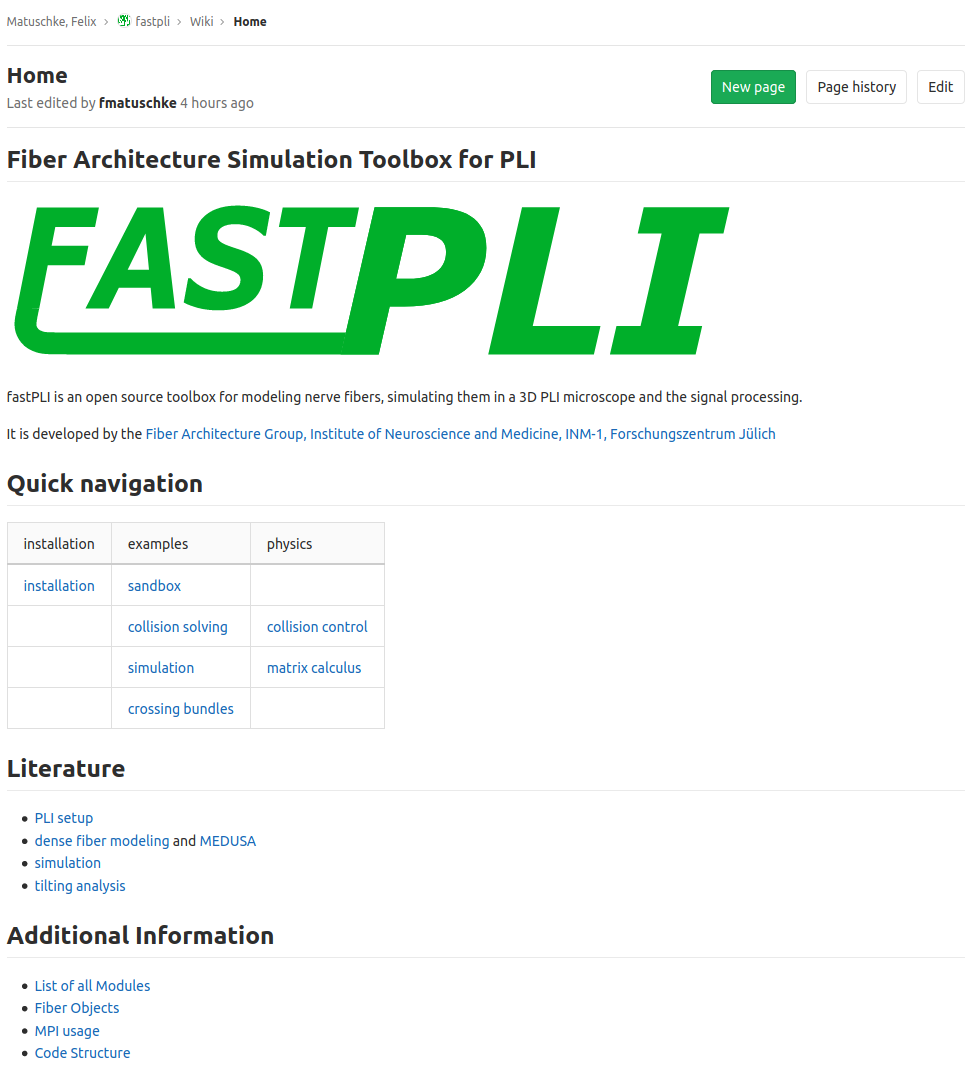
\includegraphics[width=0.95\textwidth,height=0.95\textheight,keepaspectratio,trim={400px 42px 460px 42px},clip]{gfx/fastpli/fastpli_wiki_home.png}}}
	\caption{dummy}
	\label{fig:fastpli_wiki_home}
\end{figure}
% 
\begin{figure}[!t]
    \centering
    \fbox{
    \resizebox{\textwidth}{!}{
    \begin{tabular}{c|c}
         	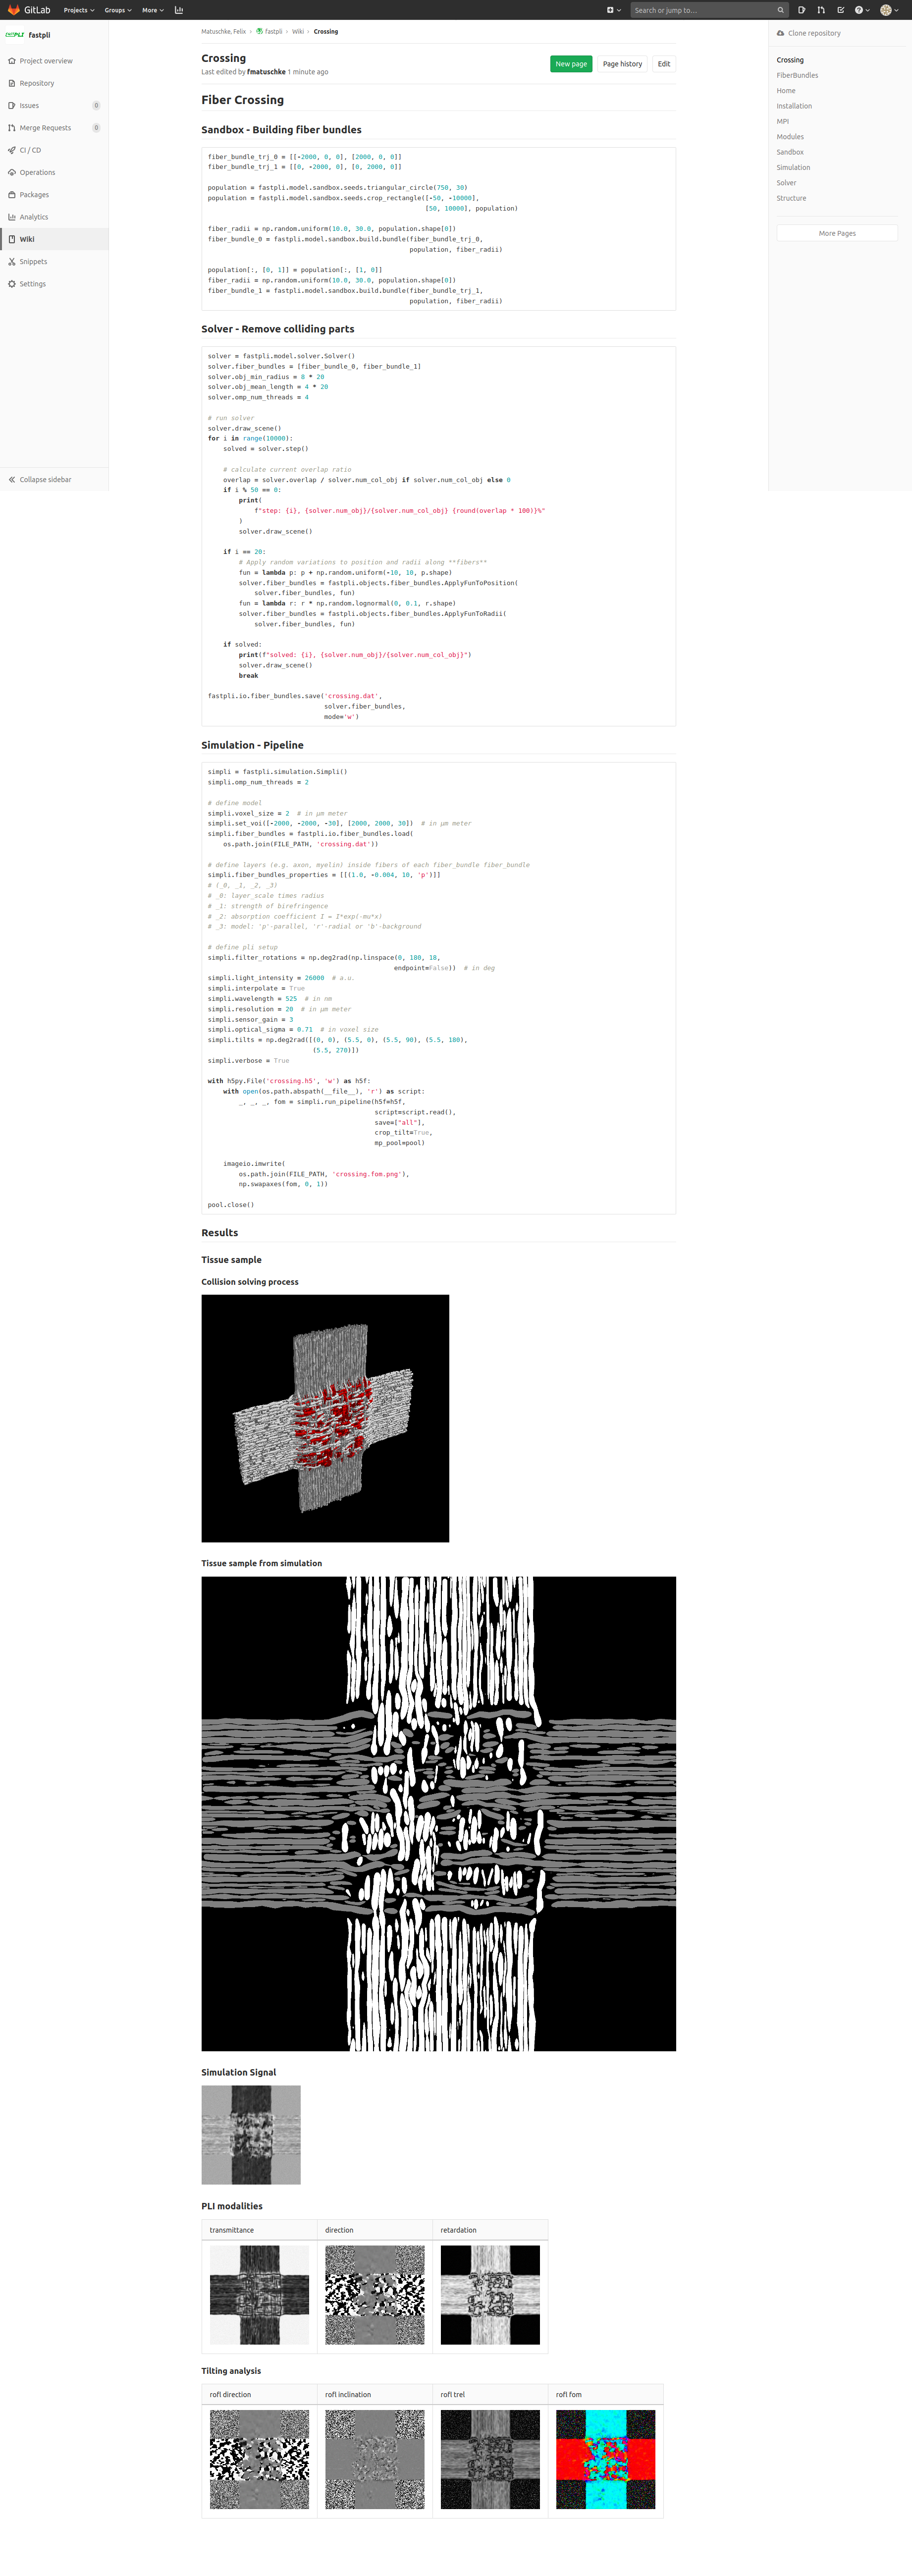
\includegraphics[width=\textwidth,height=\textheight,keepaspectratio,
         					trim={400px 2735px 460px 42px},clip]{
         						gfx/fastpli/fastpli_wiki_crossing.png} &
         	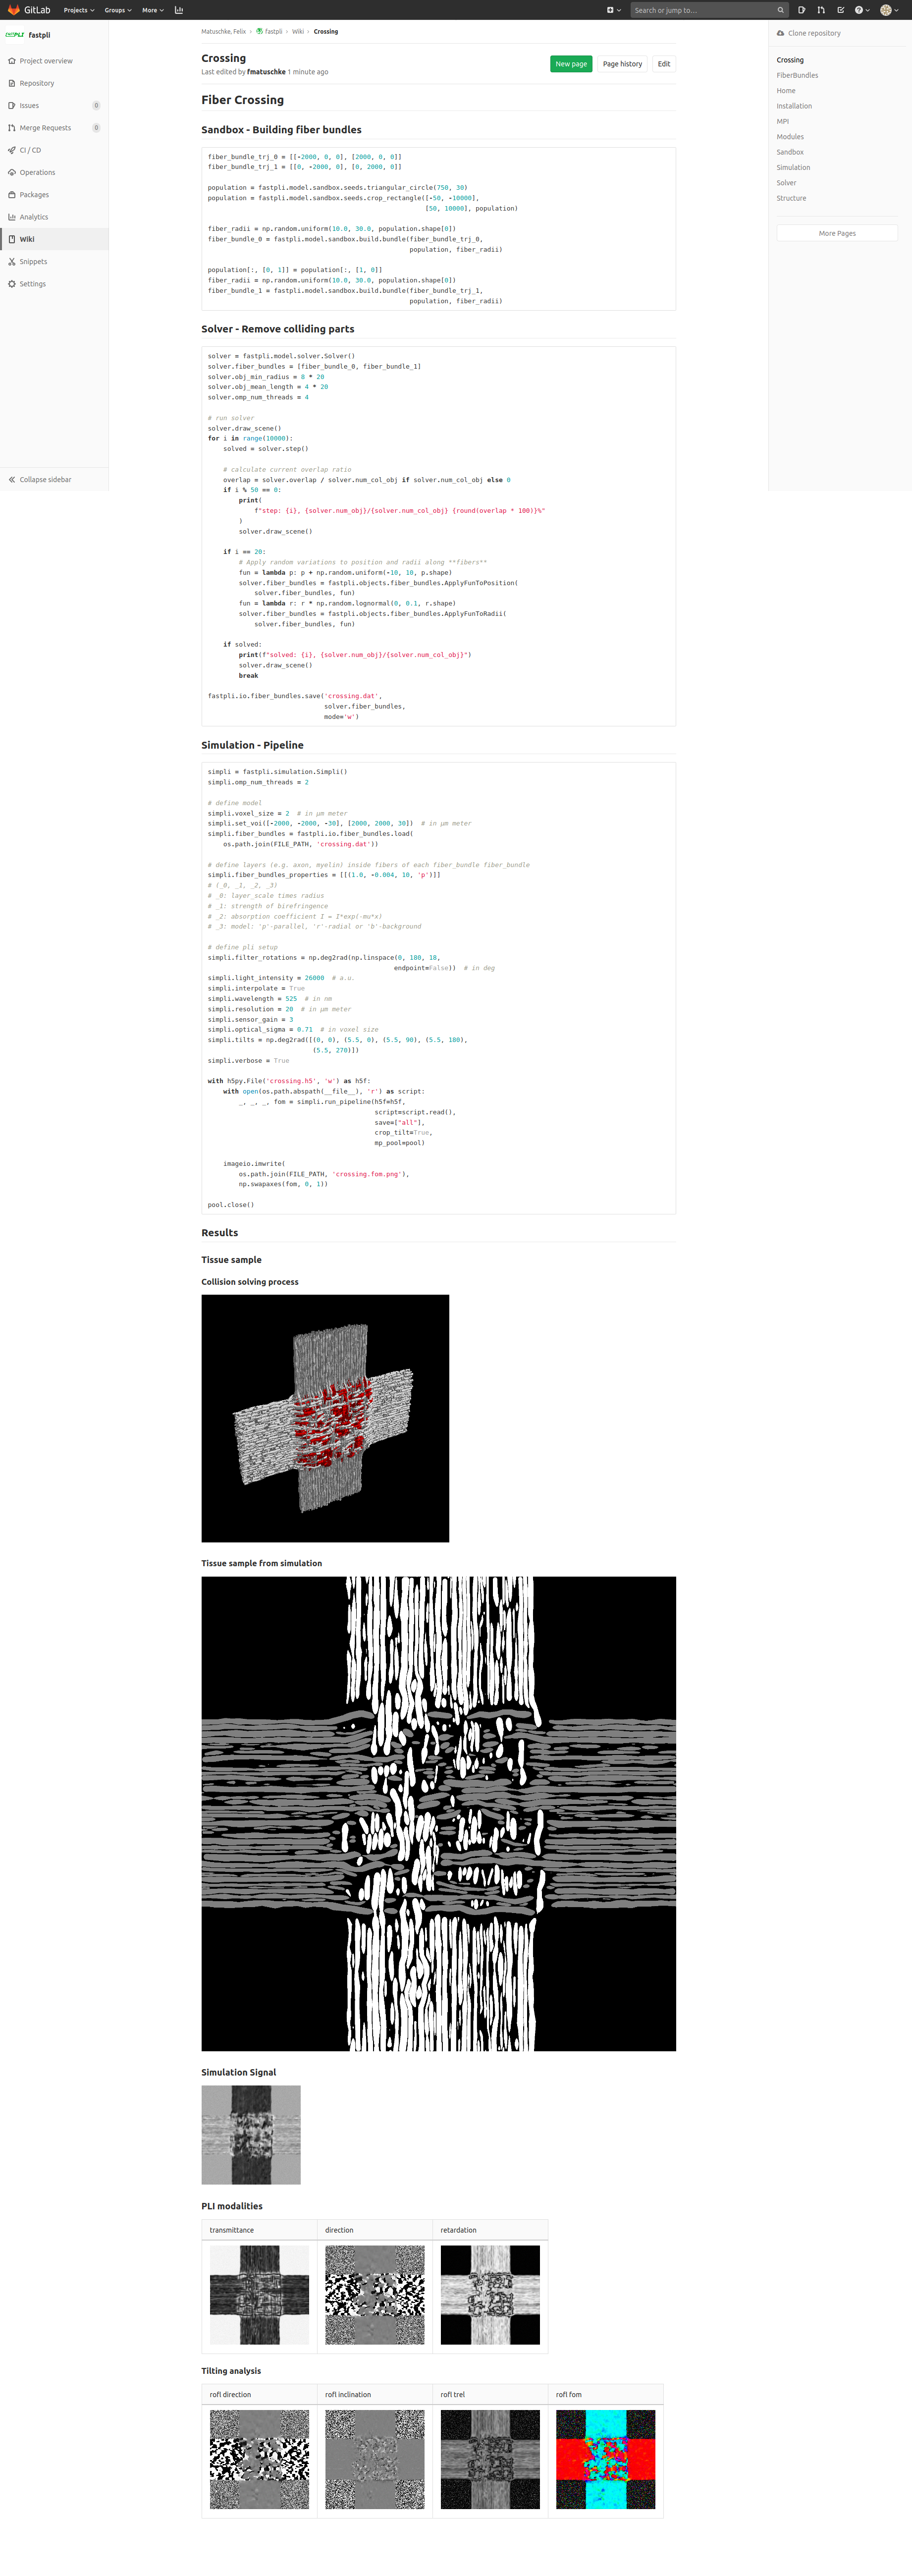
\includegraphics[width=\textwidth,height=\textheight,keepaspectratio,
         					trim={400px 42px 460px 2465px},clip]{
         						gfx/fastpli/fastpli_wiki_crossing.png}  \\
    \end{tabular}
    }}
	\caption{dummy}
	\label{fig:fastpli_wiki_crossing}
\end{figure}
% 
% 
% A Python packages is a seperated into \textit{modules}.
% A Python packages is the overhaul collection of all modules and instructions.
% Models  \begin{quote}
%     A module can contain executable statements as well as function definitions. [\,\dots] Modules can import other modules.
% \end{quote}

% \begin{figure}[!h]
% \begin{lstlisting}[language=python]
% import my-package.my-module
% \end{lstlisting}
% \label{fig:python_test}
% \caption{python test.}
% \end{figure}


%
%\begin{figure}[!t]
%	\centering
%	\resizebox{\textwidth}{!}{
%		\tikzfigure{mindmap}
%	}
%	\label{fig:mindmap}
%	\caption{mindmap.}
%\end{figure}
%
% \begin{figure}
% 	\centering
% 	\resizebox{\textwidth}{!}{
% 	\tikzfigure{uml-example}
% 	}
% \end{figure}
%
% \begin{figure}[!t]
% 	\centering
% 	\resizebox{\textwidth}{!}{
% 		\inputtikz{gfx/fastpli/fastpli_diagram}
% 	}
% 	\label{fig:fastpli_diagram}
% 	\caption{fastpli diagram.}
% \end{figure}
%
% \begin{figure}[!t]
% 	\lstinputlisting[language=python]{code/dummy.py}
% 	\label{fig:python_test}
% 	\caption{python test.}
% \end{figure}
%
%

% 
\cleardoublepage
\part{Results}
% \acbarrier
\parttoc
\setcounter{chapter}{6}
\chapter{Dense \acs{WM} modelling analysis}
\label{cha:model_analysis}
% 
\todo{veroffentlichung in intro}
% 
\itodo{reproduzieren von modellen}
% 
\section{Introduction}
% 
After describing the functionality of the \pymodule{fastpli.model}, the next task is to use these methods not only to create realistic dense \ac{WM} models, but to keep them as simple as possible due to the complexity of the tissue.
This is due to the fact that \ac{WM} contains individual nerve fibers that typically have a size in the order of about $\SI{1}{\micro\meter}$.
Therefore, in a \SI{60}{\micro\meter} voxel of a \ac{LAP} measured \ac{3D-PLI} can be image within the \ac{WM} several thousand individual nerve fibers are already present.
Considering that each nerve fiber has a unique trajectory through this volume, this means that theoretically an absurd variety of possible configurations exists.
However, due to the nature of the \ac{3D-PLI} structure, previous studies have shown that the result of the signal depends on much less degrees of freedom than each individual nerve fiber has.
\\[\baselineskip]
% 
Therefore, this work, being the first study of its kind, focuses mainly on two randomly interwoven fiber populations for \ac{3D-PLI} simulations.
Another focus is the generation of such models, whereby the computational time effort shall be kept as low as possible.
The analysis refers to the setting of the parameters for the model generation and their influence on the resulting collision-free configurations.
% 
% 
\section{Brain tissue model}
% 
To create universal reusable \ac{WM} tissue models, a practical approach is to reduce the number of parameters to a minimum.
The approach chosen here is to build cubic volumes of up to two fiber populations with individual characterization.
The most important parameter for \ac{3D-PLI} is orientation.
% 
\subsection{single fiber bundle population}
% 
A single fiber bundle population can have any orientation $O(\varphi,\alpha)$ in 3d space.
However, since $O(\varphi,\alpha) = O(\varphi+\pi,-\alpha)$ only the orientations of a hemisphere are required.
Furthermore, the experimental setup does not allow a difference between a fiber bundle population with $\varphi = \varphi_0$ and $\varphi = \varphi_1$ when the initial optical elements are rotated by $\varphi_1-\varphi_0$, unless one considers the effect of the physical expansion of the camera pixels, which is neglected here.
Therefore it is not necessary to create a single fiber population with a direction other than $\varphi = \SI{0}{\degree}$.
However, the inclination must be sampled in the range of $[0,90]\si{\degree}$.
Since the fiber bundle populations can easily be rotate from $\varphi=\SI{0}{\degree}, \alpha=\SI{0}{\degree}$ to $\varphi=\varphi_{\text{target}}, \alpha=\alpha_{\text{target}}$, it is not necessary to create individual fiber bundle configurations.
\\
%
\paragraph{fiber distribution}
To initialize the trajectories the previous introduced method for building a cubic volume is be used (see \cref{sec:cubeModelBuilding}) along the fiber bundle population orientation $F = O(\varphi, \alpha)$.
The seeding along the fiber bundle population will be randomly set with:
\begin{align}
p = \mathrm{sample}\left(\mathrm{Uniform}(\sqrt{3}*\mathit{cube\_size})\right)
\end{align}
Each fiber will have an individual radii, sampled from a \name{log normal} distribution $\mathrm{LogNorm(
\mu,\sigma)}$ (see \cref{fig:logNormal}).
Its probability desity function looks like this:
\begin{align}
\mathrm{LogNorm}(x,\mu,\sigma)=\frac{1}{\sigma x \sqrt{2\pi}}\exp\left(-\frac{(\ln(x)-\mu)^2}{2 \sigma^2}\right)
\end{align}
% 
Its property allows to multiply by a logarithmic mean value $\fiberRadiusMu=0$ to sample values which are not allowed to have negative values like a length and keeping the desired mean value $\fiberRadiusMean$:
\begin{align}
\fiberRadius = \fiberRadiusMean \cdot \mathrm{sample}\left(\mathrm{LogNorm}(\mu=0,\sigma=0.1)\right)
\end{align}
% 
\begin{figure}[!t]
\centering
\tikzset{external/export=false}
\begin{tikzpicture}[scale=1, trim axis left, trim axis right]
\begin{axis}[height=0.46\textwidth, width=0.75\textwidth,enlargelimits=false, xlabel={$x$}, ylabel={$f(x,\mu,\sigma)$}, title=${f(x,\mu,\sigma)=\frac{1}{\sigma x \sqrt{2\pi}}\exp\left(-\frac{(\ln(x)-\mu)^2}{2 \sigma^2}\right)}$,
legend style={at={(1,1)},anchor=north east},
legend cell align={left},
]
\pgfmathsetmacro{\muValue}{0}
\pgfmathsetmacro{\sigmaValue}{0.05}
\addplot[BLUE,thick,domain=0.6:1.4, samples=2*42, smooth]{1/(\sigmaValue*x*sqrt(2*pi))*exp(-(ln(x)-\muValue)^2/(2*\sigmaValue^2))}; \addlegendentry{$\mu=0.0,\sigma=0.05$}
\pgfmathsetmacro{\muValue}{0}
\pgfmathsetmacro{\sigmaValue}{0.1}
\addplot[GREEN,thick,domain=0.6:1.4, samples=2*42, smooth]{1/(\sigmaValue*x*sqrt(2*pi))*exp(-(ln(x)-\muValue)^2/(2*\sigmaValue^2))}; \addlegendentry{$\mu=0.0,\sigma=0.1$}
\end{axis}
\end{tikzpicture}
\caption[]{\itodo{check values in literatur} Probability density function of a multiplicative \name{log normal} distribution.}
\label{fig:logNormal}
\end{figure}
% 
\paragraph{fiber segmentation}
%
To split the current straight fibers into segments for the next step, the \pymodule{fastpli.model.solver} process is used.
Each fiber is split into a mean length of $\segLength$.
%
\paragraph{fiber deformation}
After the initial seeding process, and after applying the model segment length, each \name{sphere} of a fiber will be randomly changed.
The point will be randomly displaced by a normal distribution and the radii with the log normal distribution $(\mu=0,\sigma=0.05)$.
% 
\begin{align}
\begin{split}
p &= p + \mathrm{sample}\left(\mathrm{Gaus}(\mu=0,\sigma=0.05 \cdot \fiberRadiusMean)\right)\\
r &= \fiberRadius \cdot \mathrm{sample}\left(\mathrm{LogNorm}(\mu=0,\sigma=0.05)\right)
\end{split}
\end{align}
% 
This will produce a pseudo random initial configuration for the collision solving process.
% 
\subsection{dual fiber bundle populations}
The same mathematical properties as above are true for any fiber population $F$ inside a superposition.
This means, that only a differential angle between the two orientations, so called crossing angle $\modelOmega$, is needed as well as a proportion change between both populations $\modelPsi{} = N(F_0)/N(F_G)$.
% in:
% \begin{align}
%     F_G = [\modelPsi \cdot F_0] \circ [(1-\modelPsi) \cdot F_1]
% \end{align}
% 
Since the direction of the first fiber bundle population can be again neglected, only the direction and inclination of the second fiber population relative to the first is important. Therefore it was decided to build models with \modelOmega{} from ${0,10,...,90}$ and afterwords rotating the fiber orientations around the x axis (\cref{fig:twomodelpop})
% 
% \paragraph{rest}
% % 
% As described in \cref{chap5:ShapeControl} the choice of shape parameters \segLength and \segRadius are quite important. For a realistic fiber radius distribution of around \SI{0.5}{\micro\meter} the time for a \SI{60}{\micro\meter} usable cube (\SI{105}{\micro\meter} sphere) varies from several hours up to \SI{24}{\hour}.
% 
\begin{figure}[p]
\centering
\def\tikzwidth{0.42*\textwidth}
\subcaptionbox{\label{fig:modelrotcube}A spherical volume with diameter $d$ is used as boundary, so that a cube of side length $1/1.5 \cdot d$ can be cut in any orientation inside the sphere.}
[.49\textwidth]{\inputtikz{gfx/model/sphere_cube}}\hfill
\subcaptionbox{\label{fig:modelinit}Initial orientation for two fiber populations $F_0$ and $F_1$. The angle between both populations is $\Omega$. The remaining degree of freedom are taken into account by rotating the whole volume (see \cref{fig:modelrotcube})}
[.49\textwidth]{\inputtikz{gfx/model/sphere_models}}
\\
% 
\subcaptionbox{fixed first fiber population; half rotation of second fiber population}
[.49\textwidth]{\inputtikz{gfx/model/sphere_models_a}}\hfill
\subcaptionbox{\label{subfig:Test1}increasing inclination for first fiber population}
[.49\textwidth]{\inputtikz{gfx/model/sphere_models_b}}
\\
% 
\def\tikzwidth{0.35*\textwidth}
\subcaptionbox{\label{subfig:sphere:hista1} hist a}
[.49\textwidth]{\inputtikz{gfx/model/sphere_hist_a}}\hfill
\subcaptionbox{\label{subfig:sphere:histb} hist b, with applied symmetries.}
[.49\textwidth]{\inputtikz{gfx/model/sphere_hist_b}}
\caption{two population model library \itodo{centering} \itodo{e und f fertig machen}}
\label{fig:twomodelpop}
\end{figure}
% 
% \begin{figure}[t!]
% \centering
% \includegraphics[width=0.5\textwidth]{dev/gfx/htm_levels.png}
% \caption{htm}
% \label{fig:htm}
% \end{figure}
%  
% 
\subsection{Algorithmic setup}\label{sec:modelSetup}
% 
To find a usable library of two fiber populations researched main attributes are listed in \cref{tab:cube2pop} \cref{tab:cube2popSoftware} contains the parameters of the additional \pymodule{fastpli.model.solver} algorithm. All \dummy{} will be repeated five times.
\itodo{AT THE END OF EACH STEP THE VOLUME TO SOLVE IS ALWAYS CUTTED TO 105.}
% 
\begin{table}[!b]
\sisetup{parse-numbers=false,open-bracket={\{}, close-bracket={\}}, list-final-separator={,},list-pair-separator={,}}%
\centering
\pgfplotstabletypeset[%
    thesisTableStyle,
    column type=lcl,
    columns/name/.style={string type},
    columns/variable/.style={string type},
    columns/values/.style={string type},
    every head row/.style={before row=\toprule,after row=\midrule},
    every last row/.style={after row=\bottomrule},
    col sep=&,
    row sep=\\,
    % string type,
]
{name & variable & values\\
mean fiber radius & $\textcolor{violet}{\fiberRadiusMean}$ & $\SIlist{0.5;1;2;5;10}{\micro\meter}$\\
mean segment length factor & $\textcolor{violet}{\segLengthFactor}$ & $\numlist{1;2;4;8}$\\
min segment bending radii factor & $\textcolor{violet}{\segRadiusFactor}$ & $\numlist{1;2;4;8}$\\
fiber bundle distribution value & $\textcolor{violet}{\modelPsi}$ & $\numlist{0.1;0.2;...;1.0}$ \\
fiber bundle crossing angle & $\textcolor{violet}{\modelOmega}$ & $\SIlist{0;10;...;90}{\degree}$\\
}
\caption{parameter\_statistic setup and \textcolor{violet}{variables}.}
\label{tab:cube2pop}
\end{table}
% 
\begin{table}[!b]
\centering
\sisetup{open-bracket={\{}, close-bracket={\}}, list-final-separator={,},list-pair-separator={,}}%
\pgfplotstabletypeset[%
    thesisTableStyle,
    column type=l,
    columns/variable/.style={string type},
    columns/value/.style={string type},
    every head row/.style={before row=\toprule,after row=\midrule},
    every last row/.style={after row=\bottomrule},
    col sep=&,
    row sep=\\,
]
{variable & value\\
pre model diameter & $d = \SI{120}{\micro\meter}$\\
mean fiber radius & $\textcolor{violet}{\fiberRadiusMean} = \SIlist{0.5;1;2;5;10}{\micro\meter}$\\
fiber radius distribution & $\fiberRadiusSig = \SI{0.1}{}$, $\fiberRadiusMu = \SI{0}{\micro\meter}$\\
seed.distance & $2 \cdot \textcolor{violet}{\fiberRadiusMean}$\\
seed.size & $2 \cdot \mathit{volume}$\\
bundle distribution & $\textcolor{violet}{\modelPsi}$\\
bundle crossing & $\textcolor{violet}{\modelOmega}$\\
solver.obj\_mean\_length & $\textcolor{violet}{\fiberRadiusMean} \cdot \textcolor{violet}{\segLengthFactor}$\\
solver.obj\_min\_radius & $\textcolor{violet}{\fiberRadiusMean} \cdot \textcolor{violet}{\segRadiusFactor}$\\
solver.max\_steps & $\SI{100000}{}$\\
max runtime & $\SI{24}{\hour}$\\
}
\caption{parameter\_statistic setup and \textcolor{violet}{variables}.}
\label{tab:cube2popSoftware}
\end{table}
\todo{show radius distribution}
% 
\subsection{Results}
% 
\paragraph{Volume fraction}
% 
\begin{figure}[p]
\centering
\includegraphics[width=\textwidth, page=1]{dev/gfx/2/parameter_statistic_box_plot_volume.pdf}
\caption[Model characteristics]{Model characteristic for $\fiberRadius = \SI{1}{\micro\meter}$ different parameters. \itodo{\segLengthFactor{} and \segRadiusFactor{}}}
\label{fig:psbp1}
\end{figure}
% 
\cref{fig:psbp1} show the resulting volume fraction $V/V_0$ for the parameter series.
Non crossing angles $||$ achive clearly a higher fraction of $V/V_0 > 0.75$ than their counter crossing parts $cross$.
Their value also is for fibers with radii $\fiberRadius <= \SI{5}{\micro\meter}$ very stable for all five repeats.
Further the volume fraction is stable for changes along the parameter $\segLengthFactor$ and $\segRadiusFactor$. 
Only the fibers with a radius of $\fiberRadius = \SI{10}{\micro\meter}$ achive smaler fractions and slighty unstable results with Values around \dummy{}.
\\
The crossing \dummy{} show a clear decrease volume fraction along a increase of the $\segLengthFactor$ as well as a slightly decrease with increasing $\segRadiusFactor$ for all fiber radii.
The decrease with the change of $\segLengthFactor$ stabilises around $\segLengthFactor = \num{8}$.
For smaller fiber radii the repeating process is more stable as for larger radii.
\\
Overall the volume fraction stays above 0.75 for parallel and fr > 2.
For crossing fibers in this range the value stays above around 0.5.
% 
\paragraph{Time development}
% 
\begin{figure}[p]
\centering
\includegraphics[width=\textwidth, page=2]{dev/gfx/2/parameter_statistic_time_evolve.pdf}
\caption[Time development parallel]{Time development of the model generation process of parallel fiber populations. non crossing\itodo{\segLengthFactor and \segRadiusFactor}\itodo{title}\itodo{units}}
\label{fig:timeDevelopmentNone}
\end{figure}
% 
\begin{figure}[p]
\centering
\includegraphics[width=\textwidth, page=1]{dev/gfx/2/parameter_statistic_time_evolve.pdf}
\caption[Time development parallel]{Time development of the model generation process of parallel fiber populations. crossing \itodo{\segLengthFactor and \segRadiusFactor}\itodo{title}\itodo{units}\itodo{restlichen parameter anhang}}
\label{fig:timeDevelopmentCross}
\end{figure}
% 
The change in time of the properties are shown in \cref{fig:timeDevelopmentNone,fig:timeDevelopmentCross}.
Looking at only the non crossing models \cref{fig:timeDevelopmentNone} shows a linear correlation between the number of steps and the time.
All models have a step size smaller than the maximal step size, therefore are completely solved and the last plotted value corresponds to the total time consumption for each parameter set.
The change of $\segLengthFactor$ has no significant influence.
An increase in $\segRadiusFactor$ on the other side clearly increases the log(time) consumption up to several order of magnitudes.
\\
% 
Looking at the number of colliding objects they correlate with the time (non log!). 
Again a change in $\segLengthFactor$ has no significant effect and an increase in $\segRadiusFactor$ increases the time consumption up to several order of magnitudes.
\\
% 
The overlap fraction coresponts to the overlapping distance/distance in total of all remaining colliding objects.
Its value at the start is non higher of \SI{8}{\percent} \dummy{}.
The values are decreasing similar to the number of colliding objects, however not as fast.
As before, a change in $\segLengthFactor$ has no significant effect and an increase in $\segRadiusFactor$ increases the time consumption up to several order of magnitudes.
% 
The comparison to crossing models in \cref{fig:timeDevelopmentCross} shows for all parameters a very similar behavior.
The development of the number of steps is exactly as for the linear case, expect that the number of steps are higher.
fl=\dummy{} and fl= \dummy{} reach the maximal number of steps, but not the maximal time value.
\todo{human time values in plot}.
The number of objects and overlapping fraction value show a splitting behavior for a change in $\segLengthFactor$.
For smaller values the time consumption is significantly (log!) smaller.
larger values show a stagnant behavior for the parameters, however already for small values (log!).
A change in $\segRadiusFactor$  increases the time consumption up to several order of magnitudes as in the linear bundle case.
% 
% 
% 
\subsection{Discussion}
% 
The goal is to choice a set of parameters, which allow a) fast, b) collision free and c) a high volume fraction for densely fibers.
In the case of parallel fibers, the solving process is always faster than for crossing bundles.
Even thow that the number of colliding objects is more or less \dummy{} the same \comment{(ein plot?)} the needed volume to have enough space to not collide with each other is larger \dummy{}.
Therefore the distance the fiber segments have to travel is higher und the number of steps to achive this increases as well.
\\
% 
The behavior in change of the length factor \segLengthFactor{} is clearly a time advantage, since also the number ob objects is smaller.
However a larger \segLengthFactor{} results for crossing fibers as to be expected in a smaller volume fraction.
For parallel fiber is is reasonable that the volume fraction das not change, since the direction of movement for all fiber segments is radial symmetric along their main orientation axis.
Up to a fiber radii of \SI{2}{\micro\meter} the repeating measurements are stable.
Above it the resulting orientations starts to divers.
This has to to with that the volume has a fixed size of \SI{60}{\micro\meter}.
This means the number of segments is quite small, individual and the model is therefore diverge.
\\
The fiber semgent bending radii factor \segRadiusFactor{} yield to less diverse results.
Since it restrict the bending radii, it is expected, and visible in the results, that the volume fraction is very influenced, since the volume can't be optimal filled anymore.
Again changes parallel fiber orientation are almost not visible, for all analysed values.
Crossing fibers however are as expected influenced.
This is especial visible in the number of colliding objects, where the \segRadiusFactor{} splits the data into individual branches over time.
Since smaller values of \segRadiusFactor{} allow more curved geometries, this is as expected.
However this can lead to \say{strange looking} results and has to be set with an anatomical perspective. \todo{images}
\\[\baselineskip]
% 
Overall the choice of the parameters can be narrowed.
The main decision come from the crossing results.
Since most basic parameter is the length length factor \segLengthFactor{}.
Looking at the volume fraction results it should be as small as possible.
However since the difference between $\segLengthFactor=\SI{1}{}$ and $\segLengthFactor=\SI{2}{}$ is small, and a big leap is visible for $\segLengthFactor=\SI{4}{}$ one can use $\segLengthFactor=\SI{2}{}$.
The only reason to increase this value further would be a reduction in computational time.
\\
% 
The fiber radii should be as realistic to real \acs{WM} brain tissue as possible.
However to reduce the computational time further, a reduction to $r = \SI{1}{\micro\meter}$ is feasible.
It is still in the same order of magnitude to the real values (\SI{0.5}{\micro\meter}).
The \ac{3D-PLI} simulation results will show more effective metric to further restrict these parameters.
% 
The choice of the fiber banding factor is as already mentioned, more a anatomical restriction.
However it can be resend, that it has no benefit to reduce its value more then 1 or fibers can (with a small fiber segment length) move perfectly around another fiber, like horseshoe shaped.
To work against this, but not to further restrict the model geometry a value of 2 is chosen.
Therefore $\segLengthFactor = \SI{2}{}, \segLengthFactor=\SI{2}{}$ and $\fiberRadius=\SI{1}{\micro\meter}$.
\\
% 
A last remark.
An additional property to reduce the computational time is to not completely solve the model. 
Looking at the overlap fraction of the remaining overlapping segments, a value of $<\SI{1}{\percent}$ can be feasible.
This this an additional order of magnitude can be potential saved.
However, the effect inside the simulation has to be studied.
% 
\section{CPU Acceleration}
% 
\begin{figure}[!t]
\centering
\includegraphics[]{dev/gfx/4/model_solver_cubes.pdf}
\caption[speedup]{\itodo{cores, not threads} \itodo{farben?}}
\label{fig:solverSpeedup}
\end{figure}
% 
\itodo{Welche Parameter ...}
% 
As described in \dummy{} \openmp{} is used for acceleration.
This means no usage of multiple computer nodes is currently available.
\cref{fig:solverSpeedup} shows a speedup up to eight cores.
A number of two cores gives a good speedup of around $1.8$, three cores around $2.5$ and four cores around $3$.
A further incresse of core numbers does not benefit the computational time much.
This has most likely to do with the fact, that the data has to transvered between all the cores and this takes quite some time.
Even if the algorithm is especially optimized to reduce the amount of data to be copied, the paralysed instructions are often very short (\eg{} move positions), with the exception of the distance calculation.
Since all data is linear in memory, the cpu can use the full potential of the prefetcher and calculate very fast.
\\[\baselineskip]
% 
The results show, that especially to increase the volume size, other algorithms are needed. 
Here the \ac{GPU} seems to be the hardware of choice.
% 
\section{Building models for simulation}
% 
With the upper chosen model parameters the final models can be build.
To be able to study the effect of the fiber radii on the simulation, all radii are generated.
In this section the resulting orientation inside the volume, \ie{} the orientation of the fiber segments, will be analysed.
The same setup as above (see \cref{sec:modelSetup}) is chosen with fix $\segLengthFactor=\SI{2}{}$ and $\segRadiusFactor = \SI{2}{}$.
Using the rotational model from above, only fibers with a $\Psi =  0...90$ and $\Omega = 0.1...1.0$ are generated.
% 
\subsection{Results}
% 
\begin{figure}[!t]
\centering
% \resizebox{1.0\textwidth}{!}{
\includegraphics[width=\textwidth, page=1]{dev/rc1/cube_2pop_orientation_hist2d_output_cube_2pop_135_rc1_.pdf}
% }
\caption[Model orientation histograms]{distribution of fiber segment orientation in initial and resulting models for $\fiberRadius = \SI{1}{\micro\meter}$. \itodo{fit ESAG} \ITODO{these are only resulting models!}}
\label{fig:modelOrientation}
\end{figure}
% 
\begin{figure}[p]
\centering
% \resizebox{1.0\textwidth}{!}{
\includegraphics[width=\textwidth, page=1]{dev/rc1/cube_2pop_orientation_hist_output_cube_2pop_135_rc1_.pdf}
% }
\caption[Model orientation histograms]{Maximum normed distribution of fiber segment orientation in initial and resulting models. The left half circle contains the inclination $\alpha$ value, the right half the direction $\varphi$. \itodo{which norm?}}
\label{fig:modelOrientationHist1d}
\end{figure}
% 
The results are visualized in two polar axis plots in \cref{fig:modelOrientationHist1d}. On the right hemisphere the direction histogram is shown.
The left hemisphere shows the inclination distribution.
Both plots are decoupled from each other. \todo{histograms mit line plots?}
Each value is normed to the maximum of that curve so that the shape is visible.
A 3d visualized model is printed in the corner of each parameterset.
% 
The subset of results show that for all radii the fibers rich the same resulting distribution of orientations. 
These distributions are broder than the inital values and are centered around their initial orientations.
The resulting 3d visualized models show all an interwoven structure, where both fiber population orientations are clearly visible. \todo{anhang}
%  
\subsection{Discussion}
% 
\vspace{5pt}
\hrule
\vspace{6pt}
% 

% 
\cleardoublepage
\setcounter{chapter}{7}
\chapter{Simulation}
\label{cha:simulation_analysis}
% \minitoc
% 
% 
% 
This chapter contains focuses on the simulation of \ac{3D-PLI}.
The first part focuses on the definition of all necessary parameters.
A part of this is to determined how accurate the simulation has to be, i.e. the voxel size.
Following this, these parameters are used to simulate the previously generated models.
A focus is placed on the accuracy of tilt analyses for different orientations and crossing configurations.
% 
% 
% 
\itodo{reproduzieren von modellen}
% 
% 
% 
\section{Experimental Parameters}\label{sec:sim_choose_parameters}
% 
\subsection{optical resolution}
% 
An optical microscope has a certain resolution. This is often defined in the literature by Abbe diffraction limit. Ernst Abbe found out that the resolution of a light microscope is related to the wavelength of the light $\lambda$:
\begin{align}
d=\frac{ \lambda}{2 n \sin \theta} = \frac{\lambda}{2\mathrm{NA}}
\end{align}
.
$d$ is the minimal resolvable distance, $n$ the refcative index, $\theta$ the angle of a spot light. Further $n \sin \theta$ is better known as the numerical aperture $\mathrm{NA}$.
However, this only sets the maximum resolution. 
Every optical microscope has imaging errors.
The most common are lens aberration, chromatic aberration, ...
All these errors lead to a reduced resolution.
In addition, the sensor that captures the image also plays a role.
For a ccd sensor, this is the configuration of the pixels and their size.
% 
Mathematically, a resolution reduction of an image is modeled by a convolution with a Gaussian function of width $\sigma$.
It effectively blends the information into its roundness and thus onto the neighboring pixels.
It is also known as point spread function.
%
Therefore, the resolution must be determined for each experimental setup.
For this purpose, the USAF test chart is very often used to characterize the resolution of an optical image setup.
It consists of several patterns which have three slits with defined distances and widths.
The resolution can then be determined using the Rayleigh criterion, for example.
\par
% 
% 
\begin{figure}[!t]
\centering
\setlength{\tikzwidth}{0.5\textwidth}
\begin{tabular}{cc}
\inputtikz{dev/gfx/chap8/usaf_image}
&
\inputtikz{dev/gfx/chap8/usaf_line_plots}
\\
\begin{minipage}{0.45\textwidth}
\leavevmode\subcaption{\label{fig:usaf_image}microscopic image}
\end{minipage}&
\begin{minipage}{0.45\textwidth}
\leavevmode\subcaption{\label{fig:usaf_lines}centered line plots. \itodo{single line plots not good}}
\end{minipage}
\end{tabular}
\caption[USAF test chart measurement]{taorad pm. Line width: magenta: $\SI{2.19}{\micro\meter}$, yellow $\SI{1.95}{\micro\meter}$ and cyan $\SI{1.74}{\micro\meter}$. Resolution at about $\SI{1.95}{\micro\meter}$ yielding to an optical convolution of $\opticsigma = \SI{0.75}{\pixel}$.}
\label{fig:USAF}
\end{figure}
% 
\Cref{fig:usaf_image} shows a section of a captured PM image.
The highlighted areas show the key regions.
The first region corresponding to group \textrm{7\text{-}6} \raisebox{.25em}{\tikzset{external/export next=false}\tikz \draw[magenta,ultra thick,dashed](0,0)--(0.25,0);} has a line width of $\SI{2.19}{\micro\meter}$.
The second group \textrm{8\text{-}1} \raisebox{.25em}{\tikzset{external/export next=false}\tikz \draw[yellow,ultra thick,dashed](0,0)--(0.25,0);} has a line width of $\SI{1.95}{\micro\meter}$.
The final group \textrm{8\text{-}2} \raisebox{.25em}{\tikzset{external/export next=false}\tikz \draw[cyan,ultra thick,dashed](0,0)--(0.25,0);} has a line width of $\SI{1.74}{\micro\meter}$.
The intensity line profiles are shown in \cref{fig:usaf_lines}.
% 
Using the Rayleigh criterion, the resolution is in the range of the second group and thus around $\SI{1.95}{\micro\meter}$.
This reproduces the previous measurements in \cite{menzel_finite-difference_2018} \todo{master thesis?}.
As a result, the convolution to be applied is set to $\opticsigma = \SI{0.75}{\pixel}$ in the size of the resulting image pixel.
% 
% 
% 
\subsection{sensor gain}\label{sec:sensorGain}
%
\begin{figure}[!t]
\centering
\def\tikzwidth{0.75\textwidth}
\inputtikz[true]{gfx/pli/pli_focus}
\caption[intensity setup]{intensity setup. \itodo{check schematic}}
\label{fig:intensityFocus}
\end{figure}
% 
\begin{figure}[!t]
% thesis/2_simulation/0_parameter/sensor_gain.py
\centering
% 





\begin{tabular}{cc}
% 
% 1. IMAGE
\begin{tikzpicture}[baseline, trim axis left, trim axis right]
\begin{axis}[
width=0.45\textwidth,
height=0.45\textwidth,
point meta min=0,
point meta max=1670,
xmin=0,xmax=1,
ymin=0,ymax=1,
% 
hide axis,
% axis lines=center,
% % yticklabels={,,},
% axis line style={draw=none},
% tick style={draw=none},
% tick label style={gray},
% 
colorbar left,
colormap/gray,
colorbar style={%
    % axis line style={draw=none},
    % tick style={},
    % tick label style={black},
    every y tick label/.append style={font=\small},
}
% 
]
\addplot [forget plot] graphics [
xmin=0,xmax=1,
ymin=0,ymax=1,
] {dev/gfx/2/PM_000_vmin_0_vmax_1670.png};
\end{axis}
\end{tikzpicture}
&
% 
% 2. IMAGE
\begin{tikzpicture}[baseline, trim axis left, trim axis right]
\begin{axis}[%
width=0.45\textwidth,
height=0.45\textwidth,
% axis on top,
axis lines=center,
xlabel={x-pos},
ylabel={intensity},
]
\addplot[mark=none, blue] table[x index=0, y index=1] {dev/gfx/2/PM_000.dat};
\end{axis}
\end{tikzpicture}
\\
% 
% SUBCAPTIONS
\multicolumn{1}{l}{
\begin{minipage}{0.45\textwidth}
\leavevmode\subcaption{\label{fig:intensityImage}single microscopic image}
\end{minipage}}
&
\multicolumn{1}{l}{
\begin{minipage}{0.45\textwidth}
\leavevmode\subcaption{\label{fig:intensityProfile}intensity profile.}
\end{minipage}}
\end{tabular}
% 
\caption[intensity image]{y-mean intensity profile}
\label{fig:intensityMeasurement}
\end{figure}
% 
% 
\begin{figure}[!t]
% thesis/2_simulation/0_parameter/sensor_gain.py
\centering
\includegraphics[width=0.75\textwidth]{dev/gfx/2/PM_noise.png}
\caption[Noise analysis]{Noise analysis PM. $\opticgain_{\mathit{PM}} = \SI{0.1175}{}(?)$. \itodo{replot, also show microscope image}}
\label{fig:parameterModelSimGain}
\end{figure}
% 
As described in \cref{sec:ccdOptic} the optical noise has to be applied by a noise model.
In \cite{Wiese:887678} Hendrik Wiese measured the noise gain factor of the \ac{LAP} setup by measuring multiple times an image with a varieties of intensity values.
The same type of measurement and analysis is performed here on the \ac{PM} setup.

The measurements consist out of multiple images $(N=?)$. The specimen stage is covered with a fully absorbing cover, so that half of the image is dark.
Additionally the focal length is change in such a way, that the light is spread over the hole image sensor depide of the cover.
This allows to measure the full variance of intensities (see \cref{fig:intensityImage}).

The results are shown in \cref{fig:parameterModelSimGain} and show a gain value of $\opticgain_{\mathit{PM}} = \SI{0.1175}{}(?)$ which is agreement to the hardware specifics \todo{check and ref}.
% 
% 
% 
\subsection{Tissue properties}\label{sec:tissueProp}
% 
\begin{figure}[!t]
\centering
\def\tikzwidth{0.5\textwidth}
\begin{tabular}{l}
% 
\multicolumn{1}{c}{\inputtikz{gfx/data/vervet_transmittance}}
\\
\begin{minipage}{\textwidth}
\leavevmode\subcaption{\label{fig:brain_trans}transmittance}
\end{minipage}
\\
\multicolumn{1}{c}{\inputtikz{gfx/data/vervet_retardation}}
\\
\begin{minipage}{\textwidth}
\leavevmode\subcaption{\label{fig:brain_ret}retardation}
\end{minipage}
% 
\end{tabular}
\caption[Vervet monkey coronal section transmittance and retardation]{%
Vervet monkey coronal section $\SI{549}{}$.
a) transmittance, b) retardation.
The absorption coefficient and birefingence strength can be estimated from flat fibers.
Two \acsp{ROI} with \dummy{} pixels are annotated for this purpose.
\itodo{histograms?, why these two rois?}}
\label{fig:brain_ret_trans}
\end{figure}
% 
% 
\begin{figure}[!tp]
\centering
% \subcaptionbox{\label{fig:simTransValues}transmittance\itodo{WRONG IMAGE}}[.95\textwidth]{
% \includegraphics[width=0.95\textwidth]{dev/gfx/2/transmittance_PM_Vervet.pdf}} %\hfill
% \subcaptionbox{\label{fig:simRetValues}retardation}[.95\textwidth]{
\includegraphics[width=0.95\textwidth]{dev/gfx/2/retardation_PM_Vervet.pdf}
% }
\caption{simulations for Vervet PM tissue for different absorption coef and birefringence values.}
\label{fig:parameterModelSim}
\end{figure}
% 
The absorption coefficient $\absorp{}$ and the birefringence $\dn{}$ have to be estimated from the tissue to use suitable values within the simulation.
As the literature shows, these values are in the range of ... $\d{}$.
However, since the models generated here use stiff fiber segments, the volume density cannot reach as high values as in the elastic tissue.
To overcome this effect, the absorption and birefringence strengths must be increased to achieve comparable results.
\par
% 
To achieve this, the two components are measured in the experiment.
It is important to ensure that a homogeneous region is chosen.
In a coronal section, the corpus callosum is suitable for this purpose. It is the main fiber connection between the two cerebral hemispheres.
A problem with transmission is that scattering cannot be distinguished from actual absorption in this setup.
However, since this property is mathematically the same, namely a reduction in intensity along the tissue, it can still be used, but it must be remembered that it is the outdated "absorption" and not just the loss of energy in the tissue.
Additionally, the scattering is not constant for all fiber configurations and orientations \dummy{}.
Therefore, the value measured here is only valid for the same fiber configurations as the region.
However, it should be a good estimate for the magnitude of absorption in the tissue, which, as will be shown later in the simulation, is sufficient.
% 
\Cref{fig:parameterModelSim} shows a coronal section of the Vervet monkey brain \dummy(section number 549, aber was ist zu sehen, ist es in der mitte?, ...).
% 
To get a approximation of the parameters the models with a radius of $r=\SI{0.5}{\micro\meter}$ are used, which is closed to the real tissue.
% 
% 
% 
\paragraph{absorption}
% 
A relative transmittance of about $\SIrange{20}{30}{\percent}$ is present inside the \ac{ROI} of the corpus callosum \todo{show histogram}. 
The simulation parameter has to be set such as that for the models a similar transmittance value is reached.
This means, that for a $\SI{60}{\micro\meter}$ thick section the absorption coefficient $\absorp{}$ is about $\SI{30}{}$. 
Since the absorption shell be the same for larger fibers to yield the same noise and it cannot be distingioust between "no fiber matter i.e. background" and fibers the absorption coeeficient cannot be measured, and therefore the absorption will be multiplied after the simulation on the hole image. The absorption for the Roden is $\SI{8}{}$, and the human $\SI{65}{}$.

% However considering, that statistically only $\SI{75}{\percent}$ of the volume is filled, the simulation parameter has to be \dummy{}.
% \Cref{fig:simTransValues} shows different transmittance vales for different types of radii.
% 
% \ITODO{transmittance is twice as high as it should be !!! -> increase absorption coeeficient, ich glaube ich habe das bereits ersetzt}

% For r=0.5 and a Vfraction of 0.75 mu\_vervet = 30, mu\_human = 65, mu\_roden = 8
% % 
% % This yield to a absoprtion coefficient $\absorp_\textit{Vervet} = \SI{20}{\per\micro\meter}$. For the human and mouse a value of $\absorp_\textit{human} = \SI{50}{\per\micro\meter}$ and $\absorp_\textit{mouse} = \SI{10}{\per\micro\meter}$ is measured.
% 
%
% 
\paragraph{birefringence}
% 
Literature measured a birefringence of nerve fibers of around \dummy{}. 
% Scince for this simulations the models are rigide and therefore are spatially farer away from each other, this means that the tissue density is lower than in reality.
% Therefore to reach similar retardation values the birefringence value has to be increased.
To analyse the effect of the lower desity inside the models, the birefringence values is simulated at a voxel size of $\SI{0.125}{\micro\meter}$ at different values.
The results in \cref{fig:parameterModelSim} show that to reach a retardation value similar to the experimental setup of around $\SI{0.8}{}$ a birefringence value of $\SI{-0.004}{}$ for a macroscopic and $\SI{0.008}{}$ for the microscopic model should be chosen.
This is around factor 2 \todo{check} higher than literatur.
However keeping the lower density in mind and the effect of a fixed myelin radii model of $\SI{75}{\percent}$ this is still in agreement.
Looking at the different model nerve fiber radii the variance of the retardation values increase strong.
This is to be expected since the simulated tissue section has a hight of $\SI{60}{\micro\meter}$.
Therefore for a radii of $\SI{10}{\micro\meter}$ the number of tissue voxels has to vary depending on where the fibers are positioned in the volume.
For larger radii this can lead to an reduction of retardation due to the $\sin(...)$ ambiguity.
That is also the reason why the values are non normal distributed between $\si{0}$ and $\si{1}$.
%  
% 
% 
\subsection{noise}
% 
\begin{figure}[!t]
\centering
\inputtikz{gfx/data/theo_noise}
\caption[noise plot]{noise \dummy{}}
\label{fig:noiseplot}
\end{figure}
% 
From \cref{sec:sensorGain,sec:tissueProp} the noise level can be calculated.
However, when considering the different species, it is important to note that transmittance levels vary.
Rodents typically have the highest transmittance, monkeys have a lower transmittance, and humans have the lowest transmittance.
The reason for the rather low transmission of the human sections is probably due to the long post-mortem period.
\Cref{fig:noiseplot} shows a log-log plot for this purpose.
To run the simulation, a relative error of \dummy{} is used for a midrange analysis.
% 
% 
% 
\subsection{voxel size \texorpdfstring{\voxels{}}{}}
% 
% 
\begin{figure}[!tp]%p
% 2_simulation/0_parameter/fiber_radii.py
\centering
\includegraphics[width=\textwidth, page=4]{dev/gfx/2/voxel_size_plots_data_1.pdf}
\caption[voxel size model with noise]{1. $(\modelOmega=0, \modelPsi=1, \modelInc=0)$, 2. $(\modelOmega=0, \modelPsi=1, \modelInc=90)$, 3. $(\modelOmega=90, \modelPsi=0.5, \modelInc=0)$, 4. $(\modelOmega=90, \modelPsi=0.5, \modelInc=90)$: the mean difference between the Signal $\mean(\intensity(\voxels_{\mathit{ref} = \SI{0.0125}{\micro\meter}, \fiberRadius})- \intensity(\voxels, \fiberRadius))$. The mean difference is constant for smaller voxel sizes and does not start to grow significantly before $\voxels=\SI{0.125}{\micro\meter}$. \itodo{labels}}
\label{fig:voxelsizeNoise}
\end{figure}
% 
The voxel size \voxelsize{} is the main parameter for simulation accuracy.
Smaller values mean more details, more accurate optical axes, more light rays.
However, it also means an increase in memory by $O(n^3)$.
Therefore, it is advisable to choose the voxel size as small as possible, with reasonable results.
\par
% 
To investigate this effect, a simulation is performed with different types of voxel sizes from the $\SIrange{0.0125}{1.25}{\micro\meter}$.
The smallest voxel size $\SI{0.0125}{\micro\meter}$ is used as ground truth or comparison. 
However, this voxel size is so small that this is only performed for a single tissue section. \todo{which?, how much memory, ...}
The pixel size \pixelsize{} will be set to $\SI{1.25}{\micro\meter}$. \todo{other parameters}
\par
%
The results  in \cref{fig:voxelsizeNoise} show that the relative difference to the smallest \voxelsize{} increase statically after a value of \SI{0.125}{\micro\meter}.
The variance of the relative difference increases with the radius of the models as well as with the \voxelsize{}.\todo{was sind die vier unterschiedlichen plots?}
% 
In summary:
The results shown in \cref{fig:voxelsizeNoise} indicate that for noise, a voxel size smaller than $\SI{0.125}{\micro\meter}$ does not increase the accuracy with respect to the noise model chosen here.
However, this is only true for a pixel size of $\SI{1.25}{\micro\meter}$.
% 
% 
% 
\subsection{Fiber radii}
% 
\begin{figure}[!t]
\centering
\includegraphics[width=1\textwidth]{dev/gfx/sim_cube/radius_acc_compare_Vervet_PM_r.pdf}
\caption[sim acc]{ $\acc{}(GT,GT_{0.5})$, $\acc{}(SIM,GT_{0.5})$ and $\acc{}(SIM,SIM_{0.5})$. hypothese: abweichungen in GtSim bei kleinen radien dadurch, dass zwei richtungen nicht sichtbar sind? schaue dir die histogramme und odfs an. \itodo{komplett neu machen}}
\label{fig:accVervetPMr}
\end{figure}
% 
The last parameter to investigate is the fiber radius $\fiberRadius{}$ of the models.
The anatomical closes value is of course $\fiberRadius{} = \SI{0.5}{\micro\meter}$.
However to allow faster modelling processen it is feasable to analyse with which radius a difference is visiable in the microscopic setup.
To investigate this behavior the distribution of the orientation of the fiber segments was analysed.
\par
% 
\paragraph{results}
\Cref{fig:accVervetPMr} shows the ACC(GT0.5 to GT difference between the orientation of the models of different radii (always to $\fiberRadius{} = \SI{0.5}{\micro\meter}$).
the second shows the ACC(GT0.5 to SIM) and the last $\acc{}(SIM,SIM_{0.5})$.
% 
The first plot shows a very close correspondence between the GT of different radii (see y scala).
For more intermixed fiber populations (\modelPsi{} closer to $\SI{0.5}{\micro\meter}$) as well as crossing angle \modelOmega{} the \acc{} decreases slightly.
Overall the difference is almost negligible.
\par
%
Plot 2 shows a different result for the comparison between the $GT$ and $SIM$.
Here only fiber populations \modelPsi{} close to $\SI{0}{}$ or $\SI{1}{}$ have a high agreement for smaller fiber radii \fiberRadius{}.
The \acc{} decreeses with incrasing radii \fiberRadius{} down to a value of $\approx \SI{0.7}{}$.
Fiber populations with \modelPsi{} closer to 0.5 have a very low ACC parameter. For the 0.6 case the \acc{} increases slightly for increasing radii up to acc=0.6.
The crossing angle has a high impact on the acc value. 
% 
\paragraph{...}
Looking at the results from the $acc(GT,GT_{0.5})$ and $\acc{}(SIM,SIM_{0.5})$ of course $\fiberRadius=\SI{0.5}{\micro\meter}$ has a \acc{} of $\SI{0}{}$ since they are identical.
On the other hand $acc(GT,SIM_{0.5})$ shows for $\fiberRadius=\SI{0.5}{\micro\meter}$ the smallest values and highest variance for \acc{} since the fiber crossing leads to a low retardation and therefore signal lost and the analysis can't measure the in... signal.
% 
From the first and last plot show that a fiber radii of \SI{1}{\micro\meter} seems to have a little impact on the model and simulation side.
After that the simulation comparison \acc{}\todo{check if acc is defined.} value sinks drastically for fiber populations close to %\fiberPsi=\SI{0.5}{}$.
% 
The behavior between the ground truth $GT$ and and simulation $SIM$ will be closely examined in the next section.
\par
\noindent\rule{\textwidth}{2pt}
% 
\newpage
% 
% 
% 
\section{Simulation}
% 
\begin{enumerate}
\item $r=0.5$ or fabric tissue 
\begin{enumerate}
\item eine population:
\begin{enumerate}
    \item verhalten von transmittance, direction und retardierung wie model
    \item verteilung von orientierung SIM zu GT
\end{enumerate}
% 
\item zwei population:
\begin{enumerate}
    \item verhalten von transmittance, direction und retardierung wie model
    \item analyse signal ohne rauschen, zeigt rofl eine abweichung?
    \item verteilung von orientierung SIM zu GT (odf oder histogram?)
    \item groese "dunkler" Bereich
\end{enumerate}
\end{enumerate}
% 
\item $r > 0.5$ oder "fiberbundle":
\begin{enumerate}
\item zwei populationen
\begin{enumerate}
    \item verhalten von seeded fiber bundles zu solid fiber bundles
    \item sichtbarkeit von zwei orientierungen
\end{enumerate}
\end{enumerate}
% 
\item misc
\begin{enumerate}
    \item speed test
\end{enumerate}
% 
\item future discussions
\begin{enumerate}
    \item n-fiber populations
    \item fiber bundles of different radii
    \item fiber bundles with volume compressing solving steps
\end{enumerate}
\end{enumerate}
% 
% 
% 
\subsection{Parameters and execution}
% 
\begin{table}[!b]
\centering
\sisetup{open-bracket={\{}, close-bracket={\}}, list-final-separator={,},list-pair-separator={,}}%
\pgfplotstabletypeset[%
    thesisTableStyle,
    column type=l,
    columns/variable/.style={string type},
    columns/value/.style={string type},
    every head row/.style={before row=\toprule,after row=\midrule},
    every last row/.style={after row=\bottomrule},
    col sep=&,
    row sep=\\,
]
{variable & value\\
% 
simpli.voxel\_size & $\SI{0.125}{\micro\meter}$\\
simpli.pixel\_size & $\SI{1.25}{\micro\meter}$\\
simpli.voi & $[\SI{-30}{\micro\meter}, \SI{-30}{\micro\meter}, \SI{-30}{\micro\meter}], [\SI{30}{\micro\meter}, \SI{30}{\micro\meter}, \SI{30}{\micro\meter}]$\\
simpli.filter\_rotations & $\SIlist{0;20;40;60;80;100;120;160}{\degree}$\\
simpli.interpolate & \texttt{"Slerp"}\\
simpli.wavelength & $\SI{525}{\nano\meter}$\\
simpli.optical\_sigma & $\SI{0.75}{\pixel}$\\
tilt & $\SI{3.9}{\degree}$\\
simpli.light\_intensity & $\SI{8000}{}$\\
gain & $\SI{0.1175}{}$\\
% simpli.noise\_model & \texttt{lambda x:np.round(np.random.normal(x,np.sqrt(gain * x))).astype(np.uint16)}\\
simpli.noise\_model & \texttt{lambda x:np.round(np.random.normal(}\\
 & \ \ \ \ \ \texttt{x,np.sqrt(gain * x))).astype(np.uint16)}\\
fiber absorption & ('Roden', 8), ('Vervet', 30), ('Human', 65)\\
fiber model & 'r'\\
fiber birefringence & 0.008 for 'r'\\
fiber radii & (0.75, 1)\\
}
\caption{simpli parameters. \itodo{absorption ist volumenweit, nicht nur in faser}}
\label{tab:simParameters}
\end{table}
% 
% 
\Cref{tab:simParameters} lists the parameters of the simulation inside the \fastpli{} variable notation.
The values are chosen due to the discussion of \cref{sec:sim_choose_parameters}.
% 
\subsubsection{Execution}
% 
As described in \cref{Software} \fastpli{} contains a pipeline implementation. \dummy{}.
This implementation is used to calculate the discretized volumes (from generator), simulate the signal, performing the optical noise and analysis the resulting signal with \rofl{}\footnote{Source code is available in appendix \dummy{}.}.
\\
% 
The simulation were performed with a single compute node (\texttt{2x Intel(R) Xeon(R) CPU E5-4657L v2}).
% 
% 
% 
\subsection{single fiber population}
% 
In the case of a single fiber population only the inclination parameter $\modelInc{}$ is ... since no rotation and crossing angle exists.
\itodo{mehr inclination winkel fuer diesen Fall? -> JA}
% 
% 
% 
\subsubsection{orientation distribution}
% 
\begin{figure}[!tp]
\centering
\includegraphics[height=0.8\textheight]{dev/gfx/sim_cube/sim_plots_single_pop_hist.pdf} 
\caption[sim]{left: 2d log histogramm orientation from rofl analysis of simulation, right: 2d log histogramm of orientation of model segemnts. \dummy[auch als odf moeglich, aber schlechter vergeichbar; vieleicht contourplots von GT]{}}
\label{fig:single_fiber_pop_hist}
\end{figure}
% 
% 
% 
\begin{figure}[!tp]
\centering
\subcaptionbox{\label{fig:single_fiber_pop_epa_trans}transmittance}[.32\textwidth]{
\includegraphics[width=0.3\textwidth]{dev/gfx/sim_cube/sim_plots_single_pop_epa_trans.pdf}}\hfill
\subcaptionbox{\label{fig:single_fiber_pop_epa_dir}direction}[.32\textwidth]{
\includegraphics[width=0.3\textwidth]{dev/gfx/sim_cube/sim_plots_single_pop_epa_dir.pdf}}\hfill
\subcaptionbox{\label{fig:single_fiber_pop_epa_ret}retardation}[.32\textwidth]{
\includegraphics[width=0.3\textwidth]{dev/gfx/sim_cube/sim_plots_single_pop_epa_ret.pdf}}
\caption[]{\dummy[single population modalities; colors left to right: 0, 30, 60, 90 degree inclination; line: theoretical curve]{}}
\label{fig:single_fiber_pop_epa}
\end{figure}
% 
\begin{figure}[!tp]
\centering
\subcaptionbox{\label{fig:single_fiber_pop_rofl_dir}rofl direction}[.32\textwidth]{
\includegraphics[width=0.3\textwidth]{dev/gfx/sim_cube/sim_plots_single_pop_rofl_dir.pdf}}\hfill
\subcaptionbox{\label{fig:single_fiber_pop_rofl_inc}rofl inclination}[.32\textwidth]{
\includegraphics[width=0.3\textwidth]{dev/gfx/sim_cube/sim_plots_single_pop_rofl_inc.pdf}}\hfill
\subcaptionbox{\label{fig:single_fiber_pop_rofl_trel}rofl trel}[.32\textwidth]{
\includegraphics[width=0.3\textwidth]{dev/gfx/sim_cube/sim_plots_single_pop_rofl_trel.pdf}}
\caption[]{\dummy[single population rofl analysis; colors left to right: 0, 30, 60, 90 degree inclination; line: theoretical curve]{}}
\label{fig:single_fiber_pop_rofl}
\end{figure}
% 
\Cref{fig:single_fiber_pop_hist} shows the 3d fiber orientation distribution of the simulated (left) and the model ground truth (right) as a 2d polar log histogram.
The number of pixels is $48\cdot48=\SI{2304}{\pixel}$.
Looking at the simulation distribution for inclinations lower than $\SI{60}{\degree}$ the variance is very small.
It is similar to the variance of the ground truth \todo{number of segments in 60µm cube}.
However since the number of segments is much higher, and the simulation results from the "mean" signal of the light path, its distribution contains also many more orientations (keeping in mind the log scale).
Only for the steep fibers with an inclination of $\modelInc{}=\SI{90}{\degree}$ different orientation are visible for the simulation results.
The variance is similar to the ground truth of the model segments.
% 
% 
\subsubsection{pli-modalities}
% 
% 
% 
% 
\subsection{two fiber populations}
\subsection{filled fiber populations}
\subsection{misc}
\section{summary/discussion}
% 
% 
% 
% % \subsection{expected results}
% % 
% % 
% % 
% \subsection{Results}
% % 
% \itodo{other results?}
% \begin{itemize}
% \item noise(omega, gamma, ...)
% \item second orientation visible?
% \item absolute birefringence, transmittance, absorption as a f(omega)
% \item trel? abnahme der doppelbrechnung in flachen faser, bzw gegenüber f0?
% \end{itemize}
% % 
% % 
% % 
% \subsection{Retardation comparison}
% % 
% \begin{figure}[!t]
% \centering
% \inputtikz{dev/gfx/sim_cube/data_rofl}
% % \includegraphics[width=0.75\textwidth]{example-image} 
% \caption[data vs rofl]{data vs rofl}
% \label{fig:dataVsRofl}
% \end{figure}
% \itodo{show sinus plot of single pixel}
% % 
% % \begin{figure}[!tp]
% % \centering
% % \includegraphics[width=\textwidth]{dev/gfx/sim_cube/simulation_retardation_PM_Vervet_r.pdf}
% % % 
% % \begin{tikzpicture}
% %  \begin{axis}[
% %  scale only axis, width=0pt, height=0pt, hide axis,
% %  tick label style={/pgf/number format/.cd, fixed},
% %  colorbar,colormap/viridis high res,
% %  point meta min=0,
% %  point meta max=1,
% %   colorbar horizontal,
% %   colorbar style={width=0.75\textwidth},
% %   ]%
% %   {};
% %  \end{axis}
% % \end{tikzpicture}
% % % 
% % \caption[simulation results retardation]{0.5, PM, Vervet, r, retardation  \dummy{}}
% % \label{fig:sim_retardation_05_PM_Vervet_r}
% % \end{figure} 
% % 
% % 
% % 
% \subsection{Orientation comparison}
% % 
% \begin{figure}[!tp]
% \centering
% \includegraphics[width=\textwidth, trim = 115 50 115 0, clip]{dev/gfx/sim_cube/tissue_overlay_PM_Vervet_r_0.60_60.00_10.00_30.00_0.00_.pdf} 
% \caption[sim]{\dummy{}}
% \label{fig:sim_fyjsrg}
% \end{figure}
% % 
% % 
% % 
% % 
% \begin{figure}[!tp]
% \centering
% \includegraphics[height=0.8\textheight]{dev/gfx/sim_cube/test_r_0.5_species_Vervet_microscope_PM_model_r_inc_0.00_rot_0.00.pdf} 
% \caption[sim]{\dummy{}}
% \label{fig:sim_matrix_0}
% \end{figure}
% % 
% % 
% % 
% % 
% \begin{figure}[!tp]
% \centering
% \includegraphics[height=0.8\textheight]{dev/gfx/sim_cube/test_r_0.5_species_Vervet_microscope_PM_model_r_inc_90.00_rot_0.00.pdf} 
% \caption[sim]{\dummy{}}
% \label{fig:sim_matrix_90}
% \end{figure}
% % 
% % 
% % 
% % \begin{figure}[!t]
% % \begin{tikzpicture}[trim axis left, baseline]
% % \begin{axis}[%
% %     axis equal,
% %     axis lines = center,
% %     axis line style={opacity=0.0},
% %     ticks=none,
% %     view/h=145,
% %     scale uniformly strategy=units only,
% %     clip=false, % hide axis,
% %     width=10cm,
% %     height=10cm,
% %     xmin=-1,xmax=1,
% %     ymin=-1,ymax=1,
% %     zmin=-1,zmax=1,
% %     point meta min=0, point meta max=1,
% %     colormap/viridis,
% % ]
% % \addplot3[%
% %     surf,
% %     shader=interp,
% %     z buffer=sort,
% %     mesh/color input=explicit,
% %     ]
% %  table[x=x,y=y,z=z,
% %         meta=rgb,
% %         ] {dev/gfx/sim_cube/cube_2pop_psi_0.60_omega_60.00_r_10.00_v0_120_.solved_vs_0.1250_inc_30.00_rot_0.00_PM_Vervet_r.gt.dat};
% % \end{axis}
% % \end{tikzpicture}
% % \begin{tikzpicture}[trim axis left, baseline]
% % \begin{axis}[%
% %     axis equal,
% %     axis lines = center,
% %     axis line style={opacity=0.0},
% %     ticks=none,
% %     view/h=145,
% %     scale uniformly strategy=units only,
% %     clip=false, % hide axis,
% %     width=10cm,
% %     height=10cm,
% %     xmin=-1,xmax=1,
% %     ymin=-1,ymax=1,
% %     zmin=-1,zmax=1,
% %     point meta min=0, point meta max=1,
% %     colormap/viridis,
% % ]
% % \addplot3[%
% %     surf,
% %     shader=interp,
% %     z buffer=sort,
% %     mesh/color input=explicit,
% %     ]
% %  table[x=x,y=y,z=z,
% %         meta=rgb,
% %         ] {dev/gfx/sim_cube/cube_2pop_psi_0.60_omega_60.00_r_10.00_v0_120_.solved_vs_0.1250_inc_30.00_rot_0.00_PM_Vervet_r.rofl.dat};
% % \end{axis}
% % \end{tikzpicture}
% % % 
% % \caption[odf]{\dummy{}}
% % \label{fig:sim_fyjsrg}
% % \end{figure}
% % 
% % 
% % 
% % 
% \begin{figure}[!tp]
% \centering
% \includegraphics[width=\textwidth]{dev/gfx/sim_cube/simulation_analysis_hist_0.5_setup_PM_s_Vervet_m_r_acc.pdf}
% % 
% \begin{tikzpicture}
%  \begin{axis}[
%  scale only axis, width=0pt, height=0pt, hide axis,
%  tick label style={/pgf/number format/.cd, fixed},
%  colorbar,colormap/viridis high res,
%  point meta min=0,
%  point meta max=1,
%   colorbar horizontal,
%   colorbar style={width=0.75\textwidth,},
%   ]%
%   {};
%  \end{axis}
% \end{tikzpicture}
% % 
% \caption[simulation results acc]{0.5, PM, Vervet, r, acc-distance}
% \label{fig:hist_0.5_setup_PM_s_Vervet_m_r_acc}
% \end{figure}
% % 
% % 
% \begin{figure}[!tp]
% \centering
% \includegraphics[width=\textwidth]{dev/gfx/sim_cube/simulation_analysis_hist_0.5_setup_PM_s_Vervet_m_r_trans_mean.pdf}
% % 
% \begin{tikzpicture}
%  \begin{axis}[
%  scale only axis, width=0pt, height=0pt, hide axis,
%  tick label style={/pgf/number format/.cd, fixed},
%  colorbar,colormap/viridis high res,
%  point meta min=1000.24,
%  point meta max=1109.23,
%   colorbar horizontal,
%   colorbar style={width=0.75\textwidth,},
%   ]%
%   {};
%  \end{axis}
% \end{tikzpicture}
% % 
% \caption[simulation results transmittance]{0.5, PM, Vervet, r, transmittance}
% \label{fig:hist_0.5_setup_PM_s_Vervet_m_r_trans_mean}
% \end{figure}
% % 
% % 
% \begin{figure}[!tp]
% \centering
% \includegraphics[width=\textwidth]{dev/gfx/sim_cube/simulation_analysis_hist_0.5_setup_PM_s_Vervet_m_r_ret_mean.pdf}
% % 
% \begin{tikzpicture}
%  \begin{axis}[
%  scale only axis, width=0pt, height=0pt, hide axis,
%  tick label style={/pgf/number format/.cd, fixed},
%  colorbar,colormap/viridis high res,
%  point meta min=0.016,
%  point meta max=0.798,
%   colorbar horizontal,
%   colorbar style={width=0.75\textwidth,},
%   ]%
%   {};
%  \end{axis}
% \end{tikzpicture}
% % 
% \caption[simulation results ret]{0.5, PM, Vervet, r, retardation}
% \label{fig:hist_0.5_setup_PM_s_Vervet_m_r_ret_mean}
% \end{figure}
% %
% % 
% \begin{figure}[!tp]
% \centering
% \includegraphics[width=\textwidth]{dev/gfx/sim_cube/simulation_analysis_hist_0.5_setup_PM_s_Vervet_m_r_trel_mean.pdf}
% % 
% \begin{tikzpicture}
%  \begin{axis}[
%  scale only axis, width=0pt, height=0pt, hide axis,
%  tick label style={/pgf/number format/.cd, fixed},
%  colorbar,colormap/viridis high res,
%  point meta min=0,
%  point meta max=0.55,
%   colorbar horizontal,
%   colorbar style={width=0.75\textwidth,},
%   ]%
%   {};
%  \end{axis}
% \end{tikzpicture}
% % 
% \caption[simulation results trel]{0.5, PM, Vervet, r, trel}
% \label{fig:hist_0.5_setup_PM_s_Vervet_m_r_trel_mean}
% \end{figure}
% % 
% % 
% \begin{figure}[!tp]
% \centering
% \includegraphics[width=\textwidth]{dev/gfx/sim_cube/test_PM_Vervet_r_0.50_90.00_0.50_0.00_0.00_.pdf}
% \caption[simulation analysis]{\dummy{}}
% \label{fig:PM_Vervet_r_0.50_90.00_0.50_0.00_0.00}
% \end{figure}
% % 
% % 
% \begin{figure}[!tp]
% \centering
% \includegraphics[width=\textwidth]{dev/gfx/sim_cube/test_PM_Vervet_r_0.50_90.00_0.50_0.00_90.00_.pdf}
% \caption[simulation analysis]{\dummy{}}
% \label{fig:PM_Vervet_r_0.50_90.00_0.50_0.00_90.00}
% \end{figure}
% % 
% % 
% % 
% % \subsubsection{LAP}
% % % 
% % -> discussion
% % 
% % 
% % 
% \section{Computational speed}
% % 
% % 
% % 

% 
\cleardoublepage
% \part{To infinity and beyond}
% \parttoc
% \acbarrier
\setcounter{chapter}{9}
\chapter{Usecases}
\label{sec:usecases}
% \minitoc
%
\begin{itemize}
    \item dn -> trel? different density?
    \item LAP pixel size / which density, fiber configuration, ... can be identified
\end{itemize}
% 
\section{ROFL}
%
\section{Tissue Geometry in Experimental Results}
%
\section{Traktography}
%
\section{ODF}
%
\section{Dispersion}

% 
\cleardoublepage
\part{Conclusion}
% \acbarrier
\setcounter{chapter}{9}
\chapter{Discussion}
\label{sec:conclusion}
% 
\chapter{Conclusion}
\label{sec:conclusion}
%

%
% --------------------------
% Back matter
% --------------------------
%
\part{Bibliography}
\addtocontents{toc}{\vspace{\normalbaselineskip}}
{
\pdfbookmark[0]{Bibliography}{Bibliography}
\addchap{Bibliography}
% \label{sec:bibliography}
\setstretch{1.1}
\renewcommand{\bibfont}{\normalfont\small}
\setlength{\biblabelsep}{0pt}
\setlength{\bibitemsep}{0.5\baselineskip plus 0.5\baselineskip}
\printbibliography[heading=subbibliography,title={Literature},notkeyword={software}]
\newrefcontext[labelprefix={@}]
\printbibliography[heading=subbibliography,title={Software},keyword={software}]
}
% 
\cleardoublepage
\label{sec:acronyms}
\acsetup{pages/display=all}
\printacronyms[]


% %
% \cleardoublepage
% \listoffigures
% %
% \cleardoublepage
% \listoftables
% %
% \cleardoublepage
% \lstlistoflistings
%
% 
% \cleardoublepage
% %************************************************
% Declaration
%************************************************
% \pdfbookmark[0]{Declaration}{Declaration}
\addchap*{Declaration}
\label{sec:declaration}
\thispagestyle{empty}
%
Ich versichere an Eides Statt, dass die Dissertation von mir selbst{\"a}ndig und ohne unzul{\"a}ssige fremde Hilfe unter Beachtung der „Grunds{\"a}tze zur Sicherung guter wissenschaftlicher Praxis an der Heinrich-Heine-Universit{\"a}t D{\"u}sseldorf“ erstellt worden ist. \\[2cm]
%
\begin{minipage}{5cm}
	\rule{\textwidth}{1pt}
	\centering Ort, Datum
\end{minipage}
\hfill
\begin{minipage}{5cm}
	\rule{\textwidth}{1pt}
	\centering\thesisName
\end{minipage}
% \clearpage
%
\appendix\cleardoublepage
\part{Appendices}
\chapter{}%Software
\label{app:fastpli}
%
% \section{fastpli}
% \lstinputlisting[language=python, caption=src/fastpli/\_\_init\_\_.py]{code/src/fastpli/__init__.py}
% \section{fastpli/analysis}
% %\lstinputlisting[language=python, caption=src/fastpli/analysis/\_ROFL\_with\_jacobi.py]{code/src/fastpli/analysis/_ROFL_with_jacobi.py}
% \lstinputlisting[language=python, caption=src/fastpli/analysis/\_\_init\_\_.py]{code/src/fastpli/analysis/__init__.py}
% \lstinputlisting[language=python, caption=src/fastpli/analysis/affine\_transformation.py]{code/src/fastpli/analysis/affine_transformation.py}
% \lstinputlisting[language=python, caption=src/fastpli/analysis/epa.py]{code/src/fastpli/analysis/epa.py}
% \lstinputlisting[language=python, caption=src/fastpli/analysis/images.py]{code/src/fastpli/analysis/images.py}
% \lstinputlisting[language=python, caption=src/fastpli/analysis/orientation.py]{code/src/fastpli/analysis/orientation.py}
% \lstinputlisting[language=python, caption=src/fastpli/analysis/rofl.py]{code/src/fastpli/analysis/rofl.py}
% \section{fastpli/io}
% \lstinputlisting[language=python, caption=src/fastpli/io/\_\_init\_\_.py]{code/src/fastpli/io/__init__.py}
% \lstinputlisting[language=python, caption=src/fastpli/io/fiber.py]{code/src/fastpli/io/fiber.py}
% \lstinputlisting[language=python, caption=src/fastpli/io/label\_converter.py]{code/src/fastpli/io/label_converter.py}
% \section{fastpli/model}
% \lstinputlisting[language=python, caption=src/fastpli/model/\_\_init\_\_.py]{code/src/fastpli/model/__init__.py}
% \lstinputlisting[language=python, caption=src/fastpli/model/\_visualizer.py]{code/src/fastpli/model/_visualizer.py}
% \section{fastpli/model/sandbox}
% \lstinputlisting[language=python, caption=src/fastpli/model/sandbox/\_\_init\_\_.py]{code/src/fastpli/model/sandbox/__init__.py}
% \lstinputlisting[language=python, caption=src/fastpli/model/sandbox/build.py]{code/src/fastpli/model/sandbox/build.py}
% \lstinputlisting[language=python, caption=src/fastpli/model/sandbox/seeds.py]{code/src/fastpli/model/sandbox/seeds.py}
% \section{fastpli/model/solver}
% \lstinputlisting[language=python, caption=src/fastpli/model/solver/\_\_init\_\_.py]{code/src/fastpli/model/solver/__init__.py}
% \lstinputlisting[language=python, caption=src/fastpli/model/solver/\_solver.py]{code/src/fastpli/model/solver/_solver.py}
% \section{fastpli/objects}
% \lstinputlisting[language=python, caption=src/fastpli/objects/\_\_init\_\_.py]{code/src/fastpli/objects/__init__.py}
% \lstinputlisting[language=python, caption=src/fastpli/objects/fiber.py]{code/src/fastpli/objects/fiber.py}
% \lstinputlisting[language=python, caption=src/fastpli/objects/fiber\_bundle.py]{code/src/fastpli/objects/fiber_bundle.py}
% \lstinputlisting[language=python, caption=src/fastpli/objects/fiber\_bundles.py]{code/src/fastpli/objects/fiber_bundles.py}
% \section{fastpli/simulation}
% \lstinputlisting[language=python, caption=src/fastpli/simulation/\_\_init\_\_.py]{code/src/fastpli/simulation/__init__.py}
% \lstinputlisting[language=python, caption=src/fastpli/simulation/\_simpli.py]{code/src/fastpli/simulation/_simpli.py}
% \lstinputlisting[language=python, caption=src/fastpli/simulation/optic.py]{code/src/fastpli/simulation/optic.py}
% \section{fastpli/tools}
% \lstinputlisting[language=python, caption=src/fastpli/tools/\_\_init\_\_.py]{code/src/fastpli/tools/__init__.py}
% \lstinputlisting[language=python, caption=src/fastpli/tools/helper.py]{code/src/fastpli/tools/helper.py}
% \lstinputlisting[language=python, caption=src/fastpli/tools/rotation.py]{code/src/fastpli/tools/rotation.py}
% \section{include}
% \section{model}
% \section{model/solver}
% \lstinputlisting[language=c++, caption=src/model/solver/cone\_class.cpp]{code/src/model/solver/cone_class.cpp}
% \lstinputlisting[language=c++, caption=src/model/solver/fiber\_class.cpp]{code/src/model/solver/fiber_class.cpp}
% \lstinputlisting[language=c++, caption=src/model/solver/oct\_tree.cpp]{code/src/model/solver/oct_tree.cpp}
% \lstinputlisting[language=c++, caption=src/model/solver/scene.cpp]{code/src/model/solver/scene.cpp}
% \lstinputlisting[language=c++, caption=src/model/solver/world.cpp]{code/src/model/solver/world.cpp}
% \section{model/solver/bindings}
% \lstinputlisting[language=c++, caption=src/model/solver/bindings/solver\_module.cpp]{code/src/model/solver/bindings/solver_module.cpp}
% \section{objects}
% \lstinputlisting[language=c++, caption=src/objects/cell.cpp]{code/src/objects/cell.cpp}
% \lstinputlisting[language=c++, caption=src/objects/fiber.cpp]{code/src/objects/fiber.cpp}
% \section{simulation}
% \lstinputlisting[language=c++, caption=src/simulation/cell\_population.cpp]{code/src/simulation/cell_population.cpp}
% \lstinputlisting[language=c++, caption=src/simulation/fiber\_bundle.cpp]{code/src/simulation/fiber_bundle.cpp}
% \lstinputlisting[language=c++, caption=src/simulation/generator.cpp]{code/src/simulation/generator.cpp}
% \lstinputlisting[language=c++, caption=src/simulation/my\_mpi.cpp]{code/src/simulation/my_mpi.cpp}
% \lstinputlisting[language=c++, caption=src/simulation/simulator.cpp]{code/src/simulation/simulator.cpp}
% \section{simulation/bindings}
% \lstinputlisting[language=c++, caption=src/simulation/bindings/generator\_module.cpp]{code/src/simulation/bindings/generator_module.cpp}
% \lstinputlisting[language=c++, caption=src/simulation/bindings/simulator\_module.cpp]{code/src/simulation/bindings/simulator_module.cpp}
%
% \chapter{Appendix B}
% %
% \begin{figure}[!tb]
% \centering
% \resizebox{0.875\textwidth}{!}{
% \def\fiberradius{0.5}
% \inputtikz{dev/gfx/2/cube_stat.tex}}
% \caption{at fl=3 somethings wrong with the first fr value.
% Better use time, steps depends on every variable!}
% % \label{app:}
% \end{figure}
% %
% \begin{figure}[!tb]
% \centering
% \resizebox{0.875\textwidth}{!}{
% \def\fiberradius{1.0}
% \inputtikz{dev/gfx/2/cube_stat.tex}}
% \caption{at fl=3 somethings wrong with the first fr value.
% Better use time, steps depends on every variable!}
% % \label{app:}
% \end{figure}
% %
% \begin{figure}[!tb]
% \centering
% \resizebox{0.875\textwidth}{!}{
% \def\fiberradius{2.0}
% \inputtikz{dev/gfx/2/cube_stat.tex}}
% \caption{at fl=3 somethings wrong with the first fr value.
% Better use time, steps depends on every variable!}
% % \label{app:}
% \end{figure}
%
% \begin{figure}[!tb]
% \centering
% \resizebox{0.875\textwidth}{!}{
% \def\fiberradius{5.0}
% \inputtikz{dev/gfx/2/cube_stat.tex}}
% \caption{at fl=3 somethings wrong with the first fr value.
% Better use time, steps depends on every variable!}
% % \label{app:}
% \end{figure}
% %
% \begin{figure}[!tb]
% \centering
% \resizebox{0.875\textwidth}{!}{
% \def\fiberradius{10.0}
% \inputtikz{dev/gfx/2/cube_stat.tex}}
% \caption{at fl=3 somethings wrong with the first fr value.
% Better use time, steps depends on every variable!}
% % \label{app:}
% \end{figure}
%
% \chapter{Appendix C}
% \begin{figure}[!tb]
% \centering
% \resizebox{1.0\textwidth}{!}{
% \begin{tikzpicture}[>=latex]
% \node[inner sep=0pt] (image) at (0,0)
%     {\includegraphics[width=1.0\textwidth]{gfx/model/results/model_analysis.pdf}};
% \begin{scope}[overlay]
%     \draw[->,thick] ($(image.north west)-(0.25,-0.25)$) -- ++(1,0) node [midway, above] {$\Omega$};
%     \draw[->,thick] ($(image.north west)-(0.25,-0.25)$) -- ++(0,-1) node [midway, above, rotate=90] {$\Psi$};
% \end{scope}
% \path ($(image.north west) + (-.5,.5)$) -- ($(image.north east) + (.5,.5)$);
% \end{tikzpicture}
% }
% \caption{model init vs solved}
% \label{app:model_histogram}
% \end{figure}
% %
% \begin{figure}[!tb]
% \centering
% \resizebox{1.0\textwidth}{!}{
% \begin{tikzpicture}[>=latex]
% \node[inner sep=0pt] (image) at (0,0)
%     {\includegraphics[width=1.0\textwidth]{gfx/model/results/histogram.pdf}};
% \begin{scope}[overlay]
%     \draw[->,thick] ($(image.north west)-(0.25,-0.25)$) -- ++(1,0) node [midway, above] {$\Omega$};
%     \draw[->,thick] ($(image.north west)-(0.25,-0.25)$) -- ++(0,-1) node [midway, above, rotate=90] {$\Psi$};
% \end{scope}
% \path ($(image.north west) + (-.5,.5)$) -- ($(image.north east) + (.5,.5)$);
% \end{tikzpicture}
% }
% \caption{Histogram cube\_2pop\_model}
% \label{app:model_histogram}
% \end{figure}
% %
% %
% \begin{figure}[!tb]
% \centering
% \resizebox{1.0\textwidth}{!}{
% \begin{tikzpicture}[>=latex]
% \node[inner sep=0pt] (image) at (0,0)
%     {\includegraphics[width=1.0\textwidth]{gfx/model/results/voxel_size_simulation_analysis.pdf}};
% \begin{scope}[overlay]
%     \draw[->,thick] ($(image.north west)-(0.25,-0.25)$) -- ++(1,0) node [midway, above] {$voxel_size$};
%     \draw[->,thick] ($(image.north west)-(0.25,-0.25)$) -- ++(0,-1) node [midway, above, rotate=90] {$f0_inc$};
% \end{scope}
% \path ($(image.north west) + (-.5,.5)$) -- ($(image.north east) + (.5,.5)$);
% \end{tikzpicture}
% }
% \vspace{-1ex}
% \begin{center}
% \begin{tikzpicture}
%     \draw[thin] (-3.0,-0.625) rectangle (3.0,0.25);
%     \draw [green!50!black] (-2.5,0) -- (-1.5,0) node [below, midway, black] {truth};
%     \draw [red,dashed] (-0.5,0) -- (0.5,0) node [below, midway, black] {model=r};
%     \draw [blue, dash dot] (1.5,0) -- (2.5,0) node [below, midway, black] {model=p};
% \end{tikzpicture}
% \end{center}
% \caption{voxel\_size\_5\_}
% \label{app:model_histogram}
% \end{figure}
% %
% \begin{figure}[!tb]
% \centering
% \resizebox{1.0\textwidth}{!}{
% \begin{tikzpicture}[>=latex]
% \node[inner sep=0pt] (image) at (0,0)
%     {\includegraphics[width=1.0\textwidth]{gfx/simpli/results/simulation_analysis_spheres_LAP_p.pdf}};
% \begin{scope}[overlay]
%     \draw[->,thick] ($(image.north west)-(0.25,-0.25)$) -- ++(1,0) node [midway, above] {$\mathfrak{f}_0^\alpha$};
%     \draw[->,thick] ($(image.north west)-(0.25,-0.25)$) -- ++(0,-1) node [midway, above, rotate=90] {$\mathfrak{f}_0^\Psi$};
% \end{scope}
% \path ($(image.north west) + (-.5,.5)$) -- ($(image.north east) + (.5,.5)$);
% \end{tikzpicture}
% }
% \caption{Sphere LAP p}
% \label{app:model_histogram}
% \end{figure}
% %
% \begin{figure}[!tb]
% \centering
% \resizebox{1.0\textwidth}{!}{
% \begin{tikzpicture}[>=latex]
% \node[inner sep=0pt] (image) at (0,0)
%     {\includegraphics[width=1.0\textwidth]{gfx/simpli/results/simulation_analysis_spheres_LAP_r.pdf}};
% \begin{scope}[overlay]
%     \draw[->,thick] (image.north west) -- ++(1,0) node [midway, above] {$\alpha_0$};
%     \draw[->,thick] (image.north west) -- ++(0,-1) node [midway, above, rotate=90] {$\Psi_0$};
% \end{scope}
% \path ($(image.north west) + (-.5,.5)$) -- ($(image.north east) + (.5,.5)$);
% \end{tikzpicture}
% }
% \caption{Sphere LAP r}
% \label{app:model_histogram}
% \end{figure}
% %
% \begin{figure}[!tb]
% \centering
% \resizebox{1.0\textwidth}{!}{
% \begin{tikzpicture}[>=latex]
% \node[inner sep=0pt] (image) at (0,0)
%     {\includegraphics[width=1.0\textwidth]{gfx/simpli/results/simulation_analysis_spheres_PM_p.pdf}};
% \begin{scope}[overlay]
%     \draw[->,thick] ($(image.north west)-(0.25,-0.25)$) -- ++(1,0) node [midway, above] {$f_0$};
%     \draw[->,thick] ($(image.north west)-(0.25,-0.25)$) -- ++(0,-1) node [midway, above, rotate=90] {$\Psi$};
% \end{scope}
% \path ($(image.north west) + (-.5,.5)$) -- ($(image.north east) + (.5,.5)$);
% \end{tikzpicture}
% }
% \caption{Sphere PM p}
% \label{app:model_histogram}
% \end{figure}
% %
% \begin{figure}[!tb]
% \centering
% \resizebox{1.0\textwidth}{!}{
% \begin{tikzpicture}[>=latex]
% \node[inner sep=0pt] (image) at (0,0)
%     {\includegraphics[width=1.0\textwidth]{gfx/simpli/results/simulation_analysis_spheres_PM_r.pdf}};
% \begin{scope}[overlay]
%     \draw[->,thick] ($(image.north west)-(0.25,-0.25)$) -- ++(1,0) node [midway, above] {$f_0$};
%     \draw[->,thick] ($(image.north west)-(0.25,-0.25)$) -- ++(0,-1) node [midway, above, rotate=90] {$\Psi$};
% \end{scope}
% \path ($(image.north west) + (-.5,.5)$) -- ($(image.north east) + (.5,.5)$);
% \end{tikzpicture}
% }
% \caption{Sphere PM r}
% \label{app:model_histogram}
% \end{figure}
% %
% \begin{figure}[!t]
% \centering
% \resizebox{1.0\textwidth}{!}{
% \includegraphics[width=\textwidth, page=2]{dev/rc1/cube_2pop_orientation_hist2d_output_cube_2pop_135_rc1.pdf}
% }
% \caption[Model orientation histograms]{density distribution of fiber segment orientation in initial and resulting models for $\fiberRadius = \SI{1}{\micro\meter}$. \itodo{fit ESAG} \ITODO{these are only resulting models!}}
% \label{app:modelOrientation}
% \end{figure}
% %
% %
%
\chapter{} % Model analysis
\label{app:modelAnalysis}
%
%
\fakesection{Model parameter}
%
\begin{figure}[!h]
    \centering
    \includegraphics[width=1\textwidth]{dev/rc1/mpara/pre_stats_box_plot_volume_output_parameter_statistic_rc1.pdf}
    \caption{Caption}
    \label{app:appModelVolumeBoxPlot}
\end{figure}
%
% % \foreach \n in {1,3,...,10}{
% % \begin{landscape}
% \begin{figure}[!t]
% \centering
% % \resizebox{\textwidth}{!}{
% \includegraphics[width=\textwidth,page=1]{dev/rc1/mpara/pre_stats_time_evolve_all_output_parameter_statistic_rc1.pdf}
% \includegraphics[width=\textwidth,page=2]{dev/rc1/mpara/pre_stats_time_evolve_all_output_parameter_statistic_rc1.pdf}
% \end{figure}
% % \end{landscape}
%
%
\fakesection{Time evolution}
%
\setlength{\tikzwidth}{\textwidth}
\begin{sidewaysfigure}[]
\centering
\includegraphics[height=\tikzwidth,page=1]{dev/rc1/mpara/pre_stats_time_evolve_all_output_parameter_statistic_rc1.pdf}
\includegraphics[height=\tikzwidth,page=2]{dev/rc1/mpara/pre_stats_time_evolve_all_output_parameter_statistic_rc1.pdf}
\label{app:pste1}
\end{sidewaysfigure}
%
\begin{sidewaysfigure}[]
\centering
% \resizebox{\tikzwidth}{!}{
\includegraphics[height=\tikzwidth,page=3]{dev/rc1/mpara/pre_stats_time_evolve_all_output_parameter_statistic_rc1.pdf}
\includegraphics[height=\tikzwidth,page=4]{dev/rc1/mpara/pre_stats_time_evolve_all_output_parameter_statistic_rc1.pdf}
% }
\label{app:pste2}
\end{sidewaysfigure}
%
\begin{sidewaysfigure}[]
\centering
% \resizebox{\textwidth}{!}{
\includegraphics[height=\tikzwidth,page=5]{dev/rc1/mpara/pre_stats_time_evolve_all_output_parameter_statistic_rc1.pdf}
\includegraphics[height=\tikzwidth,page=6]{dev/rc1/mpara/pre_stats_time_evolve_all_output_parameter_statistic_rc1.pdf}
\label{app:pste3}
\end{sidewaysfigure}
%
\begin{sidewaysfigure}[]
\centering
% \resizebox{\textwidth}{!}{
\includegraphics[height=\tikzwidth,page=7]{dev/rc1/mpara/pre_stats_time_evolve_all_output_parameter_statistic_rc1.pdf}
\includegraphics[height=\tikzwidth,page=8]{dev/rc1/mpara/pre_stats_time_evolve_all_output_parameter_statistic_rc1.pdf}
\label{app:pste4}
\end{sidewaysfigure}
%
\begin{sidewaysfigure}[]
\centering
% \resizebox{\textwidth}{!}{
\includegraphics[height=\tikzwidth,page=9]{dev/rc1/mpara/pre_stats_time_evolve_all_output_parameter_statistic_rc1.pdf}
\includegraphics[height=\tikzwidth,page=10]{dev/rc1/mpara/pre_stats_time_evolve_all_output_parameter_statistic_rc1.pdf}
\label{app:pste5}
\end{sidewaysfigure}
%
%
\fakesection{Histogramms}
%
\begin{figure}
    \centering
    \includegraphics[width=\textwidth, page=2]{dev/rc1/cube_2pop_orientation_hist2d_output_cube_2pop_135_rc1.pdf}
    \caption{Caption}
    \label{app:modelHistOrientation}
\end{figure}[]
%
\fakesection{Speedup}
%
\begin{figure}[!t]
\centering
\includegraphics[page=2]{dev/rc1/speed/boxplot_output_r_0.5__.pkl_speedup.csv.pdf}
\caption[\code{model.Sovler} speedup]{\code{model.Sovler} speedup. The time measurements are taken after $\Delta_{\mathit{steps}}$ for the next $\SI{25}{\steps}$ for parallel $(||)$ and crossing $(\times)$ fiber configurations.}
\label{app:solverSpeedupAll}
\end{figure}
%
%
%
\fakesection{Simulation Library}
\begin{table}[htb]
\centering
\caption[Opening angle distribution]{Orientation statistic of simulation model library.}
\resizebox{\textwidth}{!}{
\pgfplotstabletypeset[%
    thesisTableStyle,
    columns={omega,psi,pop,incl_mean,incl_std,incl_25,incl_50,incl_75,phi_mean,phi_std,phi_25,phi_50,phi_75,mean,std,25,50,75},
    every head row/.style={
        before row={
            \toprule
        },
        after row={$\si{\degree}$ & & & $\si{\degree}$ & $\si{\degree}$ & $\si{\degree}$ & $\si{\degree}$ & $\si{\degree}$ & $\si{\degree}$ & $\si{\degree}$ & $\si{\degree}$ & $\si{\degree}$ & $\si{\degree}$ & $\si{\degree}$ & $\si{\degree}$ & $\si{\degree}$ & $\si{\degree}$ & $\si{\degree}$ \\ \midrule},
    },
    columns/omega/.style={column name=$\Omega$},
    columns/psi/.style={column name=$\Psi$},
    columns/mean/.style={column name=$<d\Omega>$,zerofill,precision=0},
    columns/std/.style={column name=$\sigma(d\Omega)$,zerofill,precision=0},
    columns/25/.style={column name=$25(d\Omega)$,zerofill,precision=0},
    columns/50/.style={column name=$50(d\Omega)$,zerofill,precision=0},
    columns/75/.style={column name=$75(d\Omega)$,zerofill,precision=0},
    columns/incl_mean/.style={column name=$<\alpha>$,fixed,fixed zerofill,precision=0},
    columns/incl_std/.style={column name=$\sigma(\alpha)$,fixed,fixed zerofill,precision=0},
    columns/incl_25/.style={column name=$25(\alpha)$,fixed,fixed zerofill,precision=0},
    columns/incl_50/.style={column name=$50(\alpha)$,fixed,fixed zerofill,precision=0},
    columns/incl_75/.style={column name=$75(\alpha)$,fixed,fixed zerofill,precision=0},
    columns/phi_mean/.style={column name=$<\varphi>$,fixed,fixed zerofill,precision=0},
    columns/phi_std/.style={column name=$\sigma(\varphi)$,fixed,fixed zerofill,precision=0},
    columns/phi_25/.style={column name=$25(\varphi)$,fixed,fixed zerofill,precision=0},
    columns/phi_50/.style={column name=$50(\varphi)$,fixed,fixed zerofill,precision=0},
    columns/phi_75/.style={column name=$75(\varphi)$,fixed,fixed zerofill,precision=0},
    col sep=comma,
    %
]
{dev/rc1/domega/omegas_ms_2pop.csv}
}
\label{app:modelDistribution}
\end{table}
%
% 
%
\chapter{}
\label{app:Simulation}
%
\fakesection{Tissue}
%
\begin{sidewaysfigure}[!p]
\resizebox{\textheight}{!}{
\begin{tabular}{cc}
\includegraphics[]{dev/rc1/tissue/bf_rc1_retardation_PM_Roden.pdf}&
\includegraphics[]{dev/rc1/tissue/bf_rc1_retardation_PM_Human.pdf}\\
\includegraphics[]{dev/rc1/tissue/bf_rc1_transmittance_PM_Roden.pdf}&
\includegraphics[]{dev/rc1/tissue/bf_rc1_transmittance_PM_Human.pdf}
\end{tabular}}
\end{sidewaysfigure}
%
\fakesection{Voxelsize}
%
\begin{figure}[!p]
% 2_simulation/0_parameter/fiber_radii.py
\centering
\includegraphics[width=\textwidth, page=1]{dev/rc1/voxel_size/voxel_size_plots_data_output_vs_135_0.01_6_25_vervet_r_rc1.pdf}
\caption[voxel size model with noise]{The mean difference is constant for smaller voxel sizes and does not start to grow significantly before $\voxels=\SI{0.125}{\micro\meter}$.}
\label{app:voxelsizeNoise}
\end{figure}
%
%
%
\fakesection{domega}
%
\begin{figure}[!t]
    \centering
    \includegraphics[]{dev/rc1/domega/cube_2pop_domega_analysis_all_output.pdf}
    \caption{Direction and inclination distribution of simulation model library.}
    % \label{fig:my_label}
\end{figure}
%
%
%
% %%%%%%%%%%%%%%%%%%%%%%%%%%%%%%%%%%%%%%%%%%%%%%%%%%%%%%%%%%%
% SINGLE
% %%%%%%%%%%%%%%%%%%%%%%%%%%%%%%%%%%%%%%%%%%%%%%%%%%%%%%%%%%%
%
\fakesection{Single fiber population}
%
\begin{figure}[!p]
\centering
% \begin{minipage}{0.45\textwidth}
\resizebox{\textwidth}{!}{
\rotatebox{90}{
\begin{tabular}{c|c}
\begin{tabular}{c|c}
    \includegraphics[]{dev/rc1/single/cube_2pop_135_rc1_single_plots_single_pop_hist_0.0.pdf} &
    \includegraphics[]{dev/rc1/single/cube_2pop_135_rc1_single_plots_single_pop_hist_25.0.pdf} \\
    \includegraphics[]{dev/rc1/single/cube_2pop_135_rc1_single_plots_single_pop_hist_5.0.pdf} &
    \includegraphics[]{dev/rc1/single/cube_2pop_135_rc1_single_plots_single_pop_hist_30.0.pdf} \\
    \includegraphics[]{dev/rc1/single/cube_2pop_135_rc1_single_plots_single_pop_hist_10.0.pdf} &
    \includegraphics[]{dev/rc1/single/cube_2pop_135_rc1_single_plots_single_pop_hist_35.0.pdf} \\
    \includegraphics[]{dev/rc1/single/cube_2pop_135_rc1_single_plots_single_pop_hist_15.0.pdf} &
    \includegraphics[]{dev/rc1/single/cube_2pop_135_rc1_single_plots_single_pop_hist_40.0.pdf} \\
    \includegraphics[]{dev/rc1/single/cube_2pop_135_rc1_single_plots_single_pop_hist_20.0.pdf} &
    \includegraphics[]{dev/rc1/single/cube_2pop_135_rc1_single_plots_single_pop_hist_45.0.pdf}
\end{tabular}
&
\begin{tabular}{c|c}
    \includegraphics[]{dev/rc1/single/cube_2pop_135_rc1_single_plots_single_pop_hist_50.0.pdf} &
    \includegraphics[]{dev/rc1/single/cube_2pop_135_rc1_single_plots_single_pop_hist_75.0.pdf} \\
    \includegraphics[]{dev/rc1/single/cube_2pop_135_rc1_single_plots_single_pop_hist_55.0.pdf} &
    \includegraphics[]{dev/rc1/single/cube_2pop_135_rc1_single_plots_single_pop_hist_80.0.pdf} \\
    \includegraphics[]{dev/rc1/single/cube_2pop_135_rc1_single_plots_single_pop_hist_60.0.pdf} &
    \includegraphics[]{dev/rc1/single/cube_2pop_135_rc1_single_plots_single_pop_hist_85.0.pdf} \\
    \includegraphics[]{dev/rc1/single/cube_2pop_135_rc1_single_plots_single_pop_hist_65.0.pdf} &
    \includegraphics[]{dev/rc1/single/cube_2pop_135_rc1_single_plots_single_pop_hist_90.0.pdf} \\
    \includegraphics[]{dev/rc1/single/cube_2pop_135_rc1_single_plots_single_pop_hist_70.0.pdf} &
\end{tabular}
\end{tabular}
}}
%
\caption[sim]{left: 2d log histogramm orientation from rofl analysis of simulation, right: 2d log histogramm of orientation of model segemnts. \itodo{rfc plots}}
\label{app:single_fiber_pop_hist_app}
\end{figure}
%
%
% %%%%%%%%%%%%%%%%%%%%%%%%%%%%%%%%%%%%%%%%%%%%%%%%%%%%%%%%%%%
% FLAT
% %%%%%%%%%%%%%%%%%%%%%%%%%%%%%%%%%%%%%%%%%%%%%%%%%%%%%%%%%%%
%
\fakesection{Crossing fiber population}
%
\begin{figure}[!p]
\centering
\setlength{\tikzwidth}{0.45\textwidth}
\begin{tabular}{c|c}
    \includegraphics[width=\tikzwidth]{dev/rc1/flat/cube_2pop_135_rc1_flat_plots_flat_pop_hist_omega_0.0_psi_0.3.pdf} &
    \includegraphics[width=\tikzwidth]{dev/rc1/flat/cube_2pop_135_rc1_flat_plots_flat_pop_hist_omega_50.0_psi_0.3.pdf} \\
    \includegraphics[width=\tikzwidth]{dev/rc1/flat/cube_2pop_135_rc1_flat_plots_flat_pop_hist_omega_10.0_psi_0.3.pdf} &
    \includegraphics[width=\tikzwidth]{dev/rc1/flat/cube_2pop_135_rc1_flat_plots_flat_pop_hist_omega_60.0_psi_0.3.pdf} \\
    \includegraphics[width=\tikzwidth]{dev/rc1/flat/cube_2pop_135_rc1_flat_plots_flat_pop_hist_omega_20.0_psi_0.3.pdf} &
    \includegraphics[width=\tikzwidth]{dev/rc1/flat/cube_2pop_135_rc1_flat_plots_flat_pop_hist_omega_70.0_psi_0.3.pdf} \\
    \includegraphics[width=\tikzwidth]{dev/rc1/flat/cube_2pop_135_rc1_flat_plots_flat_pop_hist_omega_30.0_psi_0.3.pdf} &
    \includegraphics[width=\tikzwidth]{dev/rc1/flat/cube_2pop_135_rc1_flat_plots_flat_pop_hist_omega_80.0_psi_0.3.pdf} \\
    \includegraphics[width=\tikzwidth]{dev/rc1/flat/cube_2pop_135_rc1_flat_plots_flat_pop_hist_omega_40.0_psi_0.3.pdf} &
    \includegraphics[width=\tikzwidth]{dev/rc1/flat/cube_2pop_135_rc1_flat_plots_flat_pop_hist_omega_90.0_psi_0.3.pdf}
\end{tabular}
%
\caption[sim]{psi=0.3; left: 2d log histogramm orientation from rofl analysis of simulation, right: 2d log histogram of orientation of model segemnts. \itodo{legende}}
\label{app:flat_03_fiber_pop_hist}
\end{figure}
%
%
%
%
\begin{figure}[!p]
\centering
\setlength{\tikzwidth}{0.45\textwidth}
\begin{tabular}{c|c}
    \includegraphics[width=\tikzwidth]{dev/rc1/flat/cube_2pop_135_rc1_flat_plots_flat_pop_hist_omega_0.0_psi_0.5.pdf} &
    \includegraphics[width=\tikzwidth]{dev/rc1/flat/cube_2pop_135_rc1_flat_plots_flat_pop_hist_omega_50.0_psi_0.5.pdf} \\
    \includegraphics[width=\tikzwidth]{dev/rc1/flat/cube_2pop_135_rc1_flat_plots_flat_pop_hist_omega_10.0_psi_0.5.pdf} &
    \includegraphics[width=\tikzwidth]{dev/rc1/flat/cube_2pop_135_rc1_flat_plots_flat_pop_hist_omega_60.0_psi_0.5.pdf} \\
    \includegraphics[width=\tikzwidth]{dev/rc1/flat/cube_2pop_135_rc1_flat_plots_flat_pop_hist_omega_20.0_psi_0.5.pdf} &
    \includegraphics[width=\tikzwidth]{dev/rc1/flat/cube_2pop_135_rc1_flat_plots_flat_pop_hist_omega_70.0_psi_0.5.pdf} \\
    \includegraphics[width=\tikzwidth]{dev/rc1/flat/cube_2pop_135_rc1_flat_plots_flat_pop_hist_omega_30.0_psi_0.5.pdf} &
    \includegraphics[width=\tikzwidth]{dev/rc1/flat/cube_2pop_135_rc1_flat_plots_flat_pop_hist_omega_80.0_psi_0.5.pdf} \\
    \includegraphics[width=\tikzwidth]{dev/rc1/flat/cube_2pop_135_rc1_flat_plots_flat_pop_hist_omega_40.0_psi_0.5.pdf} &
    \includegraphics[width=\tikzwidth]{dev/rc1/flat/cube_2pop_135_rc1_flat_plots_flat_pop_hist_omega_90.0_psi_0.5.pdf}
\end{tabular}
%
\caption[sim]{psi=0.5; left: 2d log histogramm orientation from rofl analysis of simulation, right: 2d log histogramm of orientation of model segemnts. \itodo{legende}}
\label{app:flat_05_fiber_pop_hist}
\end{figure}
%
%
%
\begin{figure}[!p]
\centering
\resizebox{\textwidth}{!}{
\begin{tabular}{cc}
\includegraphics[page=1]{dev/rc1/analysis/plots_flat_pop_output_cube_2pop_135_rc1_flat.pdf} &
\includegraphics[page=2]{dev/rc1/analysis/plots_flat_pop_output_cube_2pop_135_rc1_flat.pdf}\\
\includegraphics[page=3]{dev/rc1/analysis/plots_flat_pop_output_cube_2pop_135_rc1_flat.pdf} &
\includegraphics[page=4]{dev/rc1/analysis/plots_flat_pop_output_cube_2pop_135_rc1_flat.pdf}
\end{tabular}
}
\end{figure}
%
\begin{figure}[!p]
\centering
\resizebox{\textwidth}{!}{
\begin{tabular}{cc}
\includegraphics[page=5]{dev/rc1/analysis/plots_flat_pop_output_cube_2pop_135_rc1_flat.pdf} &
\includegraphics[page=6]{dev/rc1/analysis/plots_flat_pop_output_cube_2pop_135_rc1_flat.pdf}\\
\includegraphics[page=7]{dev/rc1/analysis/plots_flat_pop_output_cube_2pop_135_rc1_flat.pdf} &
\includegraphics[page=8]{dev/rc1/analysis/plots_flat_pop_output_cube_2pop_135_rc1_flat.pdf}
\end{tabular}
}
\end{figure}
%
\begin{figure}[]
\centering
\resizebox{\textwidth}{!}{
\begin{tabular}{cc}
\includegraphics[page=9]{dev/rc1/analysis/plots_flat_pop_output_cube_2pop_135_rc1_flat.pdf} &
\includegraphics[page=10]{dev/rc1/analysis/plots_flat_pop_output_cube_2pop_135_rc1_flat.pdf}
\end{tabular}
}
\end{figure}
%
%
% %%%%%%%%%%%%%%%%%%%%%%%%%%%%%%%%%%%%%%%%%%%%%%%%%%%%%%%%%%%
% INCLINED
% %%%%%%%%%%%%%%%%%%%%%%%%%%%%%%%%%%%%%%%%%%%%%%%%%%%%%%%%%%%
%
\fakesection{Inclined fiber population}
%
\begin{figure}[!p]
\centering
\setlength{\tikzwidth}{0.45\textwidth}
\begin{tabular}{c|c}
    \includegraphics[width=\tikzwidth]{dev/rc1/inclined/cube_2pop_135_rc1_inclined_plots_inclined_pop_hist_omega_0.0_psi_0.3.pdf} &
    \includegraphics[width=\tikzwidth]{dev/rc1/inclined/cube_2pop_135_rc1_inclined_plots_inclined_pop_hist_omega_50.0_psi_0.3.pdf} \\ \includegraphics[width=\tikzwidth]{dev/rc1/inclined/cube_2pop_135_rc1_inclined_plots_inclined_pop_hist_omega_10.0_psi_0.3.pdf} & \includegraphics[width=\tikzwidth]{dev/rc1/inclined/cube_2pop_135_rc1_inclined_plots_inclined_pop_hist_omega_60.0_psi_0.3.pdf} \\
    \includegraphics[width=\tikzwidth]{dev/rc1/inclined/cube_2pop_135_rc1_inclined_plots_inclined_pop_hist_omega_20.0_psi_0.3.pdf} &
    \includegraphics[width=\tikzwidth]{dev/rc1/inclined/cube_2pop_135_rc1_inclined_plots_inclined_pop_hist_omega_70.0_psi_0.3.pdf} \\ \includegraphics[width=\tikzwidth]{dev/rc1/inclined/cube_2pop_135_rc1_inclined_plots_inclined_pop_hist_omega_30.0_psi_0.3.pdf} & \includegraphics[width=\tikzwidth]{dev/rc1/inclined/cube_2pop_135_rc1_inclined_plots_inclined_pop_hist_omega_80.0_psi_0.3.pdf} \\
    \includegraphics[width=\tikzwidth]{dev/rc1/inclined/cube_2pop_135_rc1_inclined_plots_inclined_pop_hist_omega_40.0_psi_0.3.pdf} &
    \includegraphics[width=\tikzwidth]{dev/rc1/inclined/cube_2pop_135_rc1_inclined_plots_inclined_pop_hist_omega_90.0_psi_0.3.pdf}
\end{tabular}
%
\caption[sim]{psi=0.3; left: 2d log histogramm orientation from rofl analysis of simulation, right: 2d log histogram of orientation of model segemnts. \itodo{legende}}
\label{app:incl_03_fiber_pop_hist}
\end{figure}
%
%
%
%
\begin{figure}[!p]
\centering
\setlength{\tikzwidth}{0.45\textwidth}
\begin{tabular}{c|c}
    \includegraphics[width=\tikzwidth]{dev/rc1/inclined/cube_2pop_135_rc1_inclined_plots_inclined_pop_hist_omega_0.0_psi_0.5.pdf} &
    \includegraphics[width=\tikzwidth]{dev/rc1/inclined/cube_2pop_135_rc1_inclined_plots_inclined_pop_hist_omega_50.0_psi_0.5.pdf} \\
    \includegraphics[width=\tikzwidth]{dev/rc1/inclined/cube_2pop_135_rc1_inclined_plots_inclined_pop_hist_omega_10.0_psi_0.5.pdf} &
    \includegraphics[width=\tikzwidth]{dev/rc1/inclined/cube_2pop_135_rc1_inclined_plots_inclined_pop_hist_omega_60.0_psi_0.5.pdf} \\
    \includegraphics[width=\tikzwidth]{dev/rc1/inclined/cube_2pop_135_rc1_inclined_plots_inclined_pop_hist_omega_20.0_psi_0.5.pdf} &
    \includegraphics[width=\tikzwidth]{dev/rc1/inclined/cube_2pop_135_rc1_inclined_plots_inclined_pop_hist_omega_70.0_psi_0.5.pdf} \\
    \includegraphics[width=\tikzwidth]{dev/rc1/inclined/cube_2pop_135_rc1_inclined_plots_inclined_pop_hist_omega_30.0_psi_0.5.pdf} &
    \includegraphics[width=\tikzwidth]{dev/rc1/inclined/cube_2pop_135_rc1_inclined_plots_inclined_pop_hist_omega_80.0_psi_0.5.pdf} \\
    \includegraphics[width=\tikzwidth]{dev/rc1/inclined/cube_2pop_135_rc1_inclined_plots_inclined_pop_hist_omega_40.0_psi_0.5.pdf} &
    \includegraphics[width=\tikzwidth]{dev/rc1/inclined/cube_2pop_135_rc1_inclined_plots_inclined_pop_hist_omega_90.0_psi_0.5.pdf}
\end{tabular}
%
\caption[sim]{psi=0.5; left: 2d log histogramm orientation from rofl analysis of simulation, right: 2d log histogramm of orientation of model segemnts. \itodo{legende}}
\label{app:incl_05_fiber_pop_hist}
\end{figure}
%
%
%
\begin{figure}[!p]
\centering
\resizebox{\textwidth}{!}{
\begin{tabular}{cc}
\includegraphics[page=1]{dev/rc1/analysis/plots_inclined_pop_output_cube_2pop_135_rc1_inclined.pdf} &
\includegraphics[page=2]{dev/rc1/analysis/plots_inclined_pop_output_cube_2pop_135_rc1_inclined.pdf}\\
\includegraphics[page=3]{dev/rc1/analysis/plots_inclined_pop_output_cube_2pop_135_rc1_inclined.pdf} &
\includegraphics[page=4]{dev/rc1/analysis/plots_inclined_pop_output_cube_2pop_135_rc1_inclined.pdf}
\end{tabular}
}
\end{figure}
%
\begin{figure}[!p]
\centering
\resizebox{\textwidth}{!}{
\begin{tabular}{cc}
\includegraphics[page=5]{dev/rc1/analysis/plots_inclined_pop_output_cube_2pop_135_rc1_inclined.pdf} &
\includegraphics[page=6]{dev/rc1/analysis/plots_inclined_pop_output_cube_2pop_135_rc1_inclined.pdf}\\
\includegraphics[page=7]{dev/rc1/analysis/plots_inclined_pop_output_cube_2pop_135_rc1_inclined.pdf} &
\includegraphics[page=8]{dev/rc1/analysis/plots_inclined_pop_output_cube_2pop_135_rc1_inclined.pdf}
\end{tabular}
}
\end{figure}
%
\begin{figure}[!p]
\centering
\resizebox{\textwidth}{!}{
\begin{tabular}{cc}
\includegraphics[page=9]{dev/rc1/analysis/plots_inclined_pop_output_cube_2pop_135_rc1_inclined.pdf} &
\includegraphics[page=10]{dev/rc1/analysis/plots_inclined_pop_output_cube_2pop_135_rc1_inclined.pdf}
\end{tabular}
}
\end{figure}
%
% %
% %
%
% \newpage
% \mbox{}
%
% **************************************************
% End of Document CONTENT
% **************************************************
\end{document}
